\chapter{Sequences and Series} \label{seq:chapter}

%%%%%%%%%%%%%%%%%%%%%%%%%%%%%%%%%%%%%%%%%%%%%%%%%%%%%%%%%%%%%%%%%%%%%%%%%%%%%%

\section{Sequences and limits}
\label{sec:seqsandlims}

\sectionnotes{2.5 lectures}

Analysis is essentially about taking limits.  The most basic type of a limit
is a limit of a sequence of real numbers.
We have already seen sequences used informally.  Let us give the formal
definition.

\begin{defn}
A \emph{\myindex{sequence}} (of real numbers) is a function $x \colon \N \to
\R$.  Instead of $x(n)$, we 
usually denote the $n$th element in the sequence by $x_n$.
To denote a sequence we write%
\footnote{It is common to use $\{ x_n \}$ or $\{ x_n \}_n$ for brevity.}%
\glsadd{not:sequence}%
\begin{equation*}
\{ x_n \}_{n=1}^\infty.
\end{equation*}
%to denote a sequence, though sometimes for brevity we may use $\{ x_n \}$.

A sequence $\{ x_n \}_{n=1}^\infty$ is \emph{bounded}\index{bounded sequence} if
the underlying function is bounded.  That is, if
there exists a $B \in \R$ such that
\begin{equation*}
\abs{x_n} \leq B \qquad \text{for all } n \in \N.
\end{equation*}
In other words, the sequence $\{x_n\}_{n=1}^\infty$ is bounded whenever
the set $\{ x_n : n \in \N \}$
is bounded.
We similarly define the words
\emph{bounded below}\index{bounded below!sequence} and
\emph{bounded above}\index{bounded below!sequence}.
\end{defn}

When we need
to give a concrete sequence we often give each term as a formula in
terms of $n$.
For example, $\{ \nicefrac{1}{n} \}_{n=1}^\infty$ stands for
the sequence $1, \nicefrac{1}{2}, \nicefrac{1}{3}, \nicefrac{1}{4},
\nicefrac{1}{5}, \ldots$.
The sequence $\{ \nicefrac{1}{n} \}_{n=1}^\infty$
is a bounded sequence ($B=1$ suffices).  On the other hand the sequence
$\{ n \}_{n=1}^\infty$ stands for
$1,2,3,4,\ldots$, and this sequence is not bounded (why?).

While the notation for a sequence
is similar\footnote{\cite{BS} use $(x_n)_{n=1}^\infty$ to denote
a sequence instead of $\{ x_n \}_{n=1}^\infty$, which is what \cite{Rudin:baby} uses.
Both are common.}
to that of a set, the notions are
distinct.  For example, the sequence $\bigl\{ {(-1)}^n \bigr\}_{n=1}^\infty$ is the sequence
$-1,1,-1,1,-1,1,\ldots$, whereas the set of values, the
\emph{range of the sequence}\index{range of a sequence},
is just the set $\{ -1, 1 \}$.  We write this set
as $\bigl\{ {(-1)}^n : n \in \N \bigr\}$.
% When ambiguity can arise, we
%use the words \emph{sequence} or \emph{set} to distinguish the two
%concepts.

Another example of a sequence is the so-called \emph{\myindex{constant sequence}}.
That is a sequence $\{ c \}_{n=1}^\infty = c,c,c,c,\ldots$ consisting of a single
constant $c \in \R$ repeating indefinitely.

%We now get to the idea of a
%\emph{limit of a sequence}\index{limit!of a sequence}.
%We will see in \propref{prop:limisunique}
%that a limit, if it exists, is unique.
%It makes sense to talk about \emph{the} limit of a sequence.

\begin{defn}
A sequence $\{ x_n \}_{n=1}^\infty$ is said to \emph{converge} to a number
$x \in \R$ if for every $\epsilon > 0$, there exists an $M \in \N$ such
that $\abs{x_n - x} < \epsilon$ for all $n \geq M$.
The number $x$ is called a \emph{limit} of the sequence.
If the limit $x$ is unique, we write%
\footnote{In text, this may get rendered as $\lim_{n\to\infty} x_n$.}
\glsadd{not:limseq}%
\begin{equation*}
\lim_{n\to \infty} x_n \coloneqq x .
\end{equation*}

A sequence
that converges is said to be \emph{convergent}\index{convergent!sequence}.
Otherwise, we say the sequence \emph{diverges}
or that it is
\emph{divergent}\index{divergent!sequence}.
\end{defn}

Shortly, in \propref{prop:limisunique} we will show that the limit $x$ is always
unique if it exists.  It makes sense to talk about \emph{the} limit of
a sequence and we only need to show that the sequence converges to one
number.
For the next couple of examples, let us pretend
we have already proved that limits are unique.

Intuitively, the limit being $x$ means that eventually
every number in the sequence is close to the number $x$.  More precisely,
we get arbitrarily close to the limit, provided we go far enough in the
sequence.  It does not mean we ever reach the limit.  It is possible,
and quite common, that there is no $x_n$ in the sequence that equals the
limit $x$.
We illustrate the concept in \figureref{figsequenceconvergence}.  In the
figure we first think of the sequence as a graph, as it is a function of
$\N$.   Secondly we also plot it as a sequence of labeled points on the real
line.

\begin{myfigureht}
\subimport*{figures/}{sequence-convergence_full.pdf_t}
\caption{Illustration of convergence.
On top, we show the first ten points of the sequence as a graph
with $M$ and the interval around the limit $x$ marked.
On bottom, the points of the same sequence are marked on the
number line.\label{figsequenceconvergence}}
\end{myfigureht}

When we write $\lim_{n\to\infty} x_n = x$ for some real number $x$, we are saying two
things: First, that $\{ x_n \}_{n=1}^\infty$ is convergent, and second, that the limit is
$x$.

The definition above is one of the most important definitions in analysis,
and it is necessary to understand it perfectly.  The key point in the
definition is that given \emph{any} $\epsilon > 0$, we can find an $M$.  The
$M$ can depend on $\epsilon$, so we only pick an $M$ once we know
$\epsilon$.  Let us illustrate convergence on a few examples.

\begin{example}
The constant sequence $1,1,1,1,\ldots$ is convergent and the limit is 1.  For
every $\epsilon > 0$, we pick $M = 1$.
\end{example}

\begin{example}
Claim: \emph{The sequence $\{ \nicefrac{1}{n} \}_{n=1}^\infty$ is convergent and}
\begin{equation*}
\lim_{n\to \infty} \frac{1}{n} = 0 .
\end{equation*}
Proof: Given an $\epsilon > 0$, we find an $M \in \N$ such that
$0 < \nicefrac{1}{M} < \epsilon$
(\hyperref[thm:arch:i]{Archimedean property} at work).
Then for all $n \geq M$,
\begin{equation*}
\abs{x_n - 0} = \abs{\frac{1}{n}} = \frac{1}{n} \leq \frac{1}{M} < \epsilon .
\end{equation*}
\end{example}

\begin{example}
The sequence $\bigl\{ {(-1)}^n \bigr\}_{n=1}^\infty$ is divergent.  Proof: If there
were a limit $x$, then for $\epsilon = \frac{1}{2}$ we expect an $M$ that
satisfies the definition.  Suppose
such an $M$ exists.
Then for an even $n \geq M$ we compute
\begin{equation*}
\nicefrac{1}{2} > \abs{x_n - x}  = \abs{1 - x}
\qquad \text{and} \qquad
\nicefrac{1}{2} > \abs{x_{n+1} - x}  = \abs{-1 - x} .
\end{equation*}
But
\begin{equation*}
2 = \abs{1 - x - (-1 -x)} \leq
\abs{1 - x} + \abs{-1 -x} < \nicefrac{1}{2} + \nicefrac{1}{2} = 1 ,
\end{equation*}
and that is a contradiction.
\end{example}

\begin{prop} \label{prop:limisunique}
A convergent sequence has a unique limit.
\end{prop}

The proof of this proposition exhibits a useful technique in
analysis.  Many proofs follow the same general scheme.  We want to
show a certain quantity is zero.  We write the quantity using the 
triangle inequality as two quantities, and we estimate each one
by arbitrarily small numbers.

\begin{proof}
%NOTE: should be word for word the same as 7.3.3
Suppose $\{ x_n \}_{n=1}^\infty$ has limits $x$ and $y$.
Take an arbitrary $\epsilon > 0$.
From the definition find an $M_1$ such that for all $n \geq M_1$,
$\abs{x_n-x} < \nicefrac{\epsilon}{2}$.  Similarly, find an $M_2$
such that for all $n \geq M_2$, we have
$\abs{x_n-y} < \nicefrac{\epsilon}{2}$.
Now take an $n$ such that $n \geq M_1$ and also $n \geq M_2$, and estimate
\begin{equation*}
\begin{split}
\abs{y-x}
& =
\abs{x_n-x - (x_n -y)} \\
& \leq
\abs{x_n-x} + \abs{x_n -y} \\
& <
\frac{\epsilon}{2} + \frac{\epsilon}{2} = \epsilon .
\end{split}
\end{equation*}
As $\abs{y-x} < \epsilon$ for all $\epsilon > 0$, then $\abs{y-x} = 0$
and $y=x$.  Hence the limit (if it exists) is unique.
\end{proof}

\begin{prop}
A convergent sequence $\{ x_n \}_{n=1}^\infty$ is bounded.
\end{prop}

\begin{proof}
Suppose $\{ x_n \}_{n=1}^\infty$ converges to $x$.  Thus there exists an $M \in \N$
such that for all $n \geq M$, we have
$\abs{x_n - x} < 1$.  For $n \geq M$,
\begin{equation*}
\begin{split}
\abs{x_n} & = \abs{x_n - x + x}
\\
& \leq \abs{x_n - x} + \abs{x}
\\
& < 1 + \abs{x} .
\end{split}
\end{equation*}
The set $\bigl\{ \abs{x_1}, \abs{x_2}, \ldots, \abs{x_{M-1}} , 1+\sabs{x} \bigr\}$
is a finite set and hence let
\begin{equation*}
B \coloneqq \max \bigl\{ \abs{x_1}, \abs{x_2}, \ldots, \abs{x_{M-1}}, 1+\sabs{x} \bigr\} .
\end{equation*}
Then for all $n \in \N$,
\begin{equation*}
\abs{x_n} \leq B. \qedhere
\end{equation*}
\end{proof}

The sequence $\bigl\{ {(-1)}^n \bigr\}_{n=1}^\infty$ shows that the converse
does not hold.  A bounded sequence is not necessarily convergent.

\begin{example}
Let us show $\left\{ \frac{n^2+1}{n^2+n} \right\}_{n=1}^\infty$ converges and
\begin{equation*}
\lim_{n\to\infty} \frac{n^2+1}{n^2+n} = 1 .
\end{equation*}

Given $\epsilon > 0$,
find $M \in \N$ such that $\frac{1}{M} < \epsilon$.  Then for all $n \geq
M$,
\begin{equation*}
\begin{split}
%\abs{\frac{n^2+1}{n^2+n} - 1} & =
%\abs{\frac{n^2+1 - (n^2+n)}{n^2+n}} \\
\abs{\frac{n^2+1}{n^2+n} - 1}  =
\abs{\frac{n^2+1 - (n^2+n)}{n^2+n}}
& =
\abs{\frac{1 - n}{n^2+n}} \\
& =
\frac{n-1}{n^2+n} \\
& \leq 
\frac{n}{n^2+n} 
 =
\frac{1}{n+1}  \\
& \leq \frac{1}{n}
\leq \frac{1}{M} < \epsilon .
\end{split}
\end{equation*}
Therefore,
$\lim_{n\to\infty} \frac{n^2+1}{n^2+n} = 1$.
This example shows that sometimes to get what you want, you must throw away
some information to get a simpler estimate.
\end{example}

\subsection{Monotone sequences}

The simplest type of a sequence is a monotone sequence.  Checking that
a monotone sequence converges is as easy as checking that it is bounded.
It is also easy to find
the limit for a convergent
monotone sequence, provided we can find the supremum or infimum
of a countable set of numbers.

\begin{defn}
A sequence $\{ x_n \}_{n=1}^\infty$ is \emph{monotone increasing}\index{monotone
increasing sequence} if $x_n \leq x_{n+1}$ for all $n \in \N$.  
%
A sequence $\{ x_n \}_{n=1}^\infty$ is \emph{monotone decreasing}\index{monotone
decreasing sequence} if $x_n \geq x_{n+1}$ for all $n \in \N$.  
%
If a sequence is either monotone increasing or monotone decreasing, we
can simply say the sequence is \emph{monotone}\index{monotone
sequence}.\footnote{Some
authors use the word \emph{monotonic}\index{monotonic sequence}.}
\end{defn}

For example,
$\{ n \}_{n=1}^\infty$ is monotone increasing,
$\{ \nicefrac{1}{n} \}_{n=1}^\infty$ is monotone decreasing,
the constant sequence $\{ 1 \}_{n=1}^\infty$ is both monotone increasing and monotone
decreasing, and $\bigl\{ {(-1)}^n \bigr\}_{n=1}^\infty$ is not monotone.
First few terms of a sample monotone increasing sequence
are shown in 
\figureref{figsequenceincreasing}.

\begin{myfigureht}
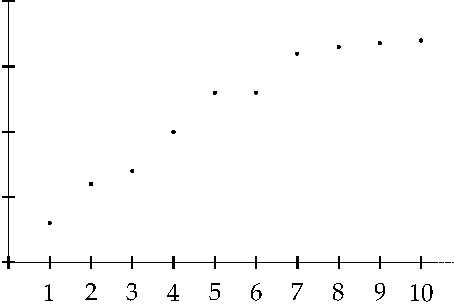
\includegraphics{figures/sequence-increasing}
\caption{First few terms of a monotone increasing sequence as a
graph.\label{figsequenceincreasing}}
\end{myfigureht}

\begin{prop} \label{prop:monotoneconv}
A monotone sequence $\{ x_n \}_{n=1}^\infty$ is bounded if and only if it is convergent.

Furthermore, if $\{ x_n \}_{n=1}^\infty$ is monotone increasing and bounded, then
\begin{equation*}
\lim_{n\to \infty} x_n = \sup \{ x_n : n \in \N \} .
\end{equation*}
If $\{ x_n \}_{n=1}^\infty$ is monotone decreasing and bounded, then
\begin{equation*}
\lim_{n\to \infty} x_n = \inf \{ x_n : n \in \N \} .
\end{equation*}
\end{prop}

\begin{proof}
Consider a monotone increasing sequence $\{ x_n \}_{n=1}^\infty$.  Suppose 
first the sequence is bounded,
that is,
the set $\{ x_n : n \in  \N \}$ is bounded.  Let
\begin{equation*}
x \coloneqq \sup \{ x_n : n \in \N \} .
\end{equation*}
Let $\epsilon > 0$ be arbitrary.  As $x$ is the supremum,
there must be at least one $M \in \N$ such that $x_{M} > x-\epsilon$.
As $\{ x_n \}_{n=1}^\infty$ is monotone increasing,
then it is easy to see (by \hyperref[induction:thm]{induction}) that
$x_n \geq x_{M}$ for all $n \geq M$.  Hence for all $n \geq M$,
\begin{equation*}
\abs{x_n-x} = x-x_n \leq x-x_{M} < \epsilon  .
\end{equation*}
So $\{ x_n \}_{n=1}^\infty$ converges to $x$.
Therefore, a bounded monotone increasing sequence converges.
For the other direction, we already proved that a convergent sequence
is bounded.

The proof for monotone decreasing sequences is left as an exercise.
\end{proof}

Note that a monotone increasing sequence $\{ x_n \}_{n=1}^\infty$
is always bounded from below since $x_1 \leq x_2 \leq \cdots \leq x_n$
for any $n$, so $x_1$ is a lower bound.  It to see if a 
monotone increasing sequence is bounded, it is enough to check if
it is bounded above.  Similarly, a monotone decreasing sequence
is always bounded from above, so it is enough to check whether it
is bounded from below.

\begin{example}
Take the sequence $\bigl\{ \frac{1}{\sqrt{n}} \bigr\}_{n=1}^\infty$.

The sequence is
bounded below as
$\frac{1}{\sqrt{n}} > 0$ for all $n \in \N$.
Let us show that it is monotone decreasing.  We start with
$\sqrt{n+1} \geq \sqrt{n}$ (why is that true?).  From this inequality
we obtain
\begin{equation*}
\frac{1}{\sqrt{n+1}} \leq \frac{1}{\sqrt{n}} .
\end{equation*}
So the sequence is monotone decreasing and bounded below (hence
bounded).  Via \propref{prop:monotoneconv} we find that the sequence is
convergent and
\begin{equation*}
\lim_{n\to \infty} \frac{1}{\sqrt{n}}
=
\inf \left\{ \frac{1}{\sqrt{n}} : n \in \N \right\} .
\end{equation*}
We already know that the infimum is greater than or equal to 0, as
0 is a lower bound.  Take a number $b \geq 0$ such
that $b \leq \frac{1}{\sqrt{n}}$ for all $n$.  We square both sides to
obtain
\begin{equation*}
b^2 \leq \frac{1}{n} \qquad \text{for all } n \in \N.
\end{equation*}
We have seen before that this implies that $b^2 \leq 0$ (a consequence
of the \hyperref[thm:arch:i]{Archimedean property}).  As $b^2 \geq 0$ as
well, we have $b^2 = 0$
and so $b = 0$.
Hence, $b=0$ is the greatest lower bound, and $\lim\limits_{n\to\infty} \frac{1}{\sqrt{n}} = 0$.
\end{example}

\begin{example}
A word of caution:  Showing that a monotone sequence is bounded
in order to use \propref{prop:monotoneconv} may be difficult.
The sequence
$\{ 1 + \nicefrac{1}{2} + \cdots + \nicefrac{1}{n} \}_{n=1}^\infty$
is a monotone increasing
sequence that grows very slowly.  We will see, once we get to series,
that this sequence has no upper bound and so does not converge.  It is not
at all obvious that this sequence has no upper bound.
\end{example}

A common example of where monotone sequences arise is the following
proposition.  The proof is left as an exercise.

\begin{prop} \label{prop:supinfseq}
Let $S \subset \R$ be a nonempty bounded set.
Then there exist monotone sequences
$\{ x_n \}_{n=1}^\infty$ and $\{ y_n \}_{n=1}^\infty$ such that $x_n, y_n \in S$ and
\begin{equation*}
\sup\,S = \lim_{n\to \infty} x_n \qquad \text{and} \qquad \inf\,S =
\lim_{n\to\infty} y_n .
\end{equation*}
\end{prop}

\subsection{Tail of a sequence}

\begin{defn}
For a sequence $\{ x_n \}_{n=1}^\infty$,
the \emph{$K$-tail} (where $K \in \N$),
or just the
\emph{tail},\index{tail of a sequence} of
$\{ x_n \}_{n=1}^\infty$ is the sequence starting at $K+1$, usually written as
\begin{equation*}
\{ x_{n+K} \}_{n=1}^\infty
\qquad \text{or} \qquad \{ x_n \}_{n=K+1}^\infty .
\end{equation*}
\end{defn}

For example, the $4$-tail of $\{ \nicefrac{1}{n} \}_{n=1}^\infty$ is
$\nicefrac{1}{5}, \nicefrac{1}{6}, \nicefrac{1}{7}, \nicefrac{1}{8},
\ldots$.  The $0$-tail of a sequence is the sequence itself.
The convergence and the limit of a sequence only depends on its tail.

\begin{prop}
Let $\{ x_n \}_{n=1}^\infty$ be a sequence.  Then the following
statements are equivalent:
\begin{enumerate}[(i)]
\item \label{prop:ktail:i}
The sequence $\{ x_n \}_{n=1}^\infty$ converges.
\item \label{prop:ktail:ii}
The $K$-tail $\{ x_{n+K} \}_{n=1}^\infty$ converges for all $K \in \N$.
\item \label{prop:ktail:iii}
The $K$-tail $\{ x_{n+K} \}_{n=1}^\infty$ converges for some $K \in \N$.
\end{enumerate}
Furthermore, if any (and hence all) of the limits exist, then for all $K \in \N$
\begin{equation*}
\lim_{n\to \infty} x_n = \lim_{n \to \infty} x_{n+K} .
\end{equation*}
\end{prop}

\begin{proof}
It is clear that
\ref{prop:ktail:ii} implies \ref{prop:ktail:iii}.
We will therefore show first that
\ref{prop:ktail:i}
implies
\ref{prop:ktail:ii},
and then we will show that
\ref{prop:ktail:iii}
implies
\ref{prop:ktail:i}.  That is, 
%mbxSTARTIGNORE
\begin{equation*}
\begin{tikzcd}[row sep=0pt]
& \text{\ref{prop:ktail:ii}} \ar[dr, Rightarrow] & \\
\text{\ref{prop:ktail:i}} \ar[ur, Rightarrow, "\text{to prove}"] & &
\text{\ref{prop:ktail:iii}} \ar[ll, Rightarrow, "\text{to prove}"] 
\end{tikzcd}
\end{equation*}
%mbxENDIGNORE
%mbxlatex \begin{center}
%mbxlatex \subimport*{figures/}{tail_of_sequence_cd.pdf_t}
%mbxlatex \end{center}
In the process we will also show that the limits are equal.

We start with \ref{prop:ktail:i} implies \ref{prop:ktail:ii}.
Suppose $\{x_n \}_{n=1}^\infty$ converges to some $x \in \R$.
Let $K \in \N$ be arbitrary, and
define $y_n \coloneqq x_{n+K}$.  We wish to show that $\{ y_n \}_{n=1}^\infty$ converges
to $x$.
Given an $\epsilon > 0$, there exists an $M \in \N$ such that
$\abs{x-x_n} < \epsilon$ for all $n \geq M$.
Note that $n \geq M$ implies $n+K \geq M$.  Therefore, for
all $n \geq M$, we have
\begin{equation*}
\abs{x-y_n} = \abs{x-x_{n+K}} < \epsilon .
\end{equation*}
Consequently, $\{ y_n \}_{n=1}^\infty$ converges to $x$.

Let us move to \ref{prop:ktail:iii} implies \ref{prop:ktail:i}.
Let $K \in \N$ be given, define
$y_n \coloneqq x_{n+K}$, and suppose that $\{ y_n \}_{n=1}^\infty$ converges to $x \in \R$.
That is, given an $\epsilon > 0$, there exists an $M' \in \N$ such that
$\abs{x-y_n} < \epsilon$ for all $n \geq M'$.
Let $M \coloneqq M'+K$.  Then $n \geq M$ implies $n-K \geq M'$.
Thus, whenever $n \geq M$, we have
\begin{equation*}
\abs{x-x_n} = \abs{x-y_{n-K}} < \epsilon.
\end{equation*}
Therefore, $\{ x_n \}_{n=1}^\infty$ converges to $x$.
\end{proof}

At the end of the day, the limit does not care about how the sequence begins, it only
cares about the tail of the sequence.  The beginning of the sequence
may be arbitrary.

For example, the sequence defined by $x_n \coloneqq \frac{n}{n^2+16}$ is decreasing
if we start at $n=4$ (it is increasing before).  That is:
$\{ x_n \}_{n=1}^\infty =
\nicefrac{1}{17},
\nicefrac{1}{10},
\nicefrac{3}{25},
\nicefrac{1}{8},
\nicefrac{5}{41},
\nicefrac{3}{26},
\nicefrac{7}{65},
\nicefrac{1}{10},
\nicefrac{9}{97},
\nicefrac{5}{58},\ldots$, and 
\begin{equation*}
\nicefrac{1}{17} <
\nicefrac{1}{10} <
\nicefrac{3}{25} <
\nicefrac{1}{8} >
\nicefrac{5}{41} >
\nicefrac{3}{26} >
\nicefrac{7}{65} >
\nicefrac{1}{10} >
\nicefrac{9}{97} >
\nicefrac{5}{58} > \ldots .
\end{equation*}
If we throw away the first 3 terms
and look at the 3-tail, it is decreasing.  The proof is left as an exercise.  Since the 3-tail
is monotone and bounded below by zero, it is convergent, and therefore the sequence is convergent.

\subsection{Subsequences}

It is useful to sometimes consider only some terms of a sequence.
A subsequence of $\{ x_n \}_{n=1}^\infty$ is a sequence that contains
only some of the numbers from $\{ x_n \}_{n=1}^\infty$ in the same order.

\begin{defn}
Let $\{ x_n \}_{n=1}^\infty$ be a sequence.
Let $\{ n_i \}_{i=1}^\infty$ be a strictly increasing sequence of natural
numbers, that is, $n_i < n_{i+1}$ for all $i \in \N$ (in other words $n_1 < n_2 < n_3 < \cdots$).  
The sequence
\begin{equation*}
\{ x_{n_i} \}_{i=1}^\infty
\end{equation*}
is called \glsadd{not:subsequence}
a \emph{\myindex{subsequence}} of $\{ x_n \}_{n=1}^\infty$.
\end{defn}

So the subsequence is the sequence $x_{n_1},x_{n_2},x_{n_3},\ldots$.
Consider the sequence $\{ \nicefrac{1}{n} \}_{n=1}^\infty$.  The sequence
$\{ \nicefrac{1}{3i} \}_{i=1}^\infty$ is a subsequence.  To see how these two
sequences fit in the definition, take $n_i \coloneqq 3i$,
that is, $\{ n_i \}_{i=1}^\infty$ is the
sequence $3,6,9,12,\ldots$.  
The numbers $x_{n_i}$ in the
subsequence must come from the original sequence.  So $1,0,\nicefrac{1}{3},0,
\nicefrac{1}{5},\ldots$
is not a subsequence of $\{ \nicefrac{1}{n} \}_{n=1}^\infty$.  Similarly, order
must be preserved.  So
the sequence $1,\nicefrac{1}{3},\nicefrac{1}{2},\nicefrac{1}{5},\ldots$
is not a subsequence of $\{ \nicefrac{1}{n} \}_{n=1}^\infty$.

A tail of a sequence is one special type of a subsequence.  For an arbitrary
subsequence, we have the following proposition about convergence.

\begin{prop} \label{prop:seqtosubseq}
If $\{ x_n \}_{n=1}^\infty$ is a convergent sequence,
then every subsequence $\{ x_{n_i} \}_{i=1}^\infty$ is also convergent, and
\begin{equation*}
\lim_{n\to \infty} x_n = 
\lim_{i\to \infty} x_{n_i} .
\end{equation*}
\end{prop}

\begin{proof}
Suppose $\lim_{n\to \infty} x_n = x$.  So for every
$\epsilon > 0$, there is an $M \in \N$ such that for all $n \geq M$,
\begin{equation*}
\abs{x_n - x} < \epsilon .
\end{equation*}
It is not hard to prove (do it!) by \hyperref[induction:thm]{induction} that
$n_i \geq i$ for all $i \in \N$.  Hence $i \geq M$ implies $n_i \geq M$.  Thus,
for all $i \geq M$,
\begin{equation*}
\abs{x_{n_i} - x} < \epsilon ,
\end{equation*}
and we are done.
\end{proof}

\begin{example}
Existence of a convergent subsequence does not imply
convergence of the sequence itself.
Take the sequence $0,1,0,1,0,1,\ldots$.  That is,
$x_n = 0$ if $n$ is odd, and $x_n = 1$ if $n$ is even.  The sequence
$\{ x_n \}_{n=1}^\infty$ is divergent; however, the subsequence
$\{ x_{2i} \}_{i=1}^\infty$ converges to 1 and the subsequence
$\{ x_{2i+1} \}_{i=1}^\infty$ converges to 0.  Compare \propref{seqconvsubseqconv:prop}.
\end{example}

\subsection{Exercises}

\begin{exnote}
In the following exercises, feel free to use what you know from calculus to
find the limit, if it exists.  But you must \emph{prove}
that you
found the correct limit, or prove that the sequence is divergent.
\end{exnote}

\begin{exercise}
Is the sequence
$\{ 3n \}_{n=1}^\infty$
bounded?  Prove or disprove.
\end{exercise}

\begin{exercise}
Is the sequence
$\{ n \}_{n=1}^\infty$
convergent?  If so, what is the limit?
\end{exercise}

\begin{exercise}
Is the sequence
$\left\{ \dfrac{{(-1)}^n}{2n} \right\}_{n=1}^\infty$
convergent?  If so, what is the limit?
\end{exercise}

\begin{exercise}
Is the sequence
$\{ 2^{-n} \}_{n=1}^\infty$
convergent?  If so, what is the limit?
\end{exercise}

\begin{exercise}
Is the sequence
$\left\{ \dfrac{n}{n+1} \right\}_{n=1}^\infty$
convergent?  If so, what is the limit?
\end{exercise}

\begin{exercise}
Is the sequence
$\left\{ \dfrac{n}{n^2+1} \right\}_{n=1}^\infty$
convergent?  If so, what is the limit?
\end{exercise}

\begin{exercise} \label{exercise:absconv}
Let $\{ x_n \}_{n=1}^\infty$ be a sequence.
\begin{enumerate}[a)]
\item Show that $\lim\limits_{n\to\infty} x_n = 0$ (that is, the limit exists and is zero)
if and only if $\lim\limits_{n\to\infty} \abs{x_n} = 0$.
\item Find an example such that $\{ \abs{x_n} \}_{n=1}^\infty$ converges and
$\{ x_n \}_{n=1}^\infty$
diverges.
\end{enumerate}
\end{exercise}

\begin{exercise}
Is the sequence
$\left\{ \dfrac{2^n}{n!} \right\}_{n=1}^\infty$
convergent?  If so, what is the limit?
\end{exercise}

\begin{exercise}
Show that the sequence
$\left\{ \dfrac{1}{\sqrt[3]{n}} \right\}_{n=1}^\infty$ is monotone and bounded.  Then use
\propref{prop:monotoneconv} to find the limit.
\end{exercise}

\begin{exercise}
Show that the sequence
$\left\{ \dfrac{n+1}{n} \right\}_{n=1}^\infty$
is monotone and bounded.  Then use
\propref{prop:monotoneconv} to find the limit.
\end{exercise}

\begin{exercise}
Finish the proof of \propref{prop:monotoneconv} for monotone decreasing
sequences.
\end{exercise}

\begin{exercise}
Prove \propref{prop:supinfseq}.
\end{exercise}

\begin{exercise}
Let $\{ x_n \}_{n=1}^\infty$ be a convergent monotone sequence.  Suppose 
there exists a $k \in \N$ such that
\begin{equation*}
\lim_{n\to \infty} x_n = x_k .
\end{equation*}
Show that $x_n = x_k$ for all $n \geq k$.
\end{exercise}

\begin{exercise}
\pagebreak[2]
Find a convergent subsequence of the sequence
$\bigl\{ {(-1)}^n \bigr\}_{n=1}^\infty$.
\end{exercise}

\begin{exercise}
Let $\{x_n\}_{n=1}^\infty$ be a sequence defined by
\begin{equation*}
x_n \coloneqq 
\begin{cases}
n               & \text{if } n \text{ is odd} , \\
\nicefrac{1}{n} & \text{if } n \text{ is even} .
\end{cases}
\avoidbreak
\end{equation*}
\begin{enumerate}[a)]
\item Is the sequence bounded? (prove or disprove)
\item Is there a convergent subsequence?  If so, find it.
\end{enumerate}
\end{exercise}

\begin{exercise}
\pagebreak[2]
Let $\{ x_n \}_{n=1}^\infty$ be a sequence.
Suppose there are two convergent subsequences $\{ x_{n_i} \}_{i=1}^\infty$ and
$\{ x_{m_i} \}_{i=1}^\infty$.  Suppose 
\begin{equation*}
\lim_{i\to\infty} x_{n_i} = a
\qquad \text{and} \qquad
\lim_{i\to\infty} x_{m_i} = b,
\end{equation*}
where $a \not= b$.  Prove that $\{ x_n \}_{n=1}^\infty$ is not convergent, without
using \propref{prop:seqtosubseq}.
\end{exercise}

\begin{exercise}[Tricky]
Find a sequence $\{ x_n \}_{n=1}^\infty$ such that for every $y \in \R$, there exists a
subsequence $\{ x_{n_i} \}_{i=1}^\infty$ converging to $y$.
\end{exercise}

\begin{exercise}[Easy]
Let $\{ x_n \}_{n=1}^\infty$ be a sequence and $x \in \R$.
Suppose for every $\epsilon > 0$, there is an $M$ such that
$\abs{x_n-x} \leq \epsilon$ for all $n \geq M$.
Show that $\lim\limits_{n\to\infty} x_n = x$.
\end{exercise}

\begin{exercise}[Easy]
Let $\{ x_n \}_{n=1}^\infty$ be a sequence and $x \in \R$ such that
there exists a $k \in \N$ such that for all $n \geq k$,
$x_n = x$.  Prove that $\{ x_n \}_{n=1}^\infty$ converges to $x$.
\end{exercise}

\begin{exercise}
Let $\{ x_n \}_{n=1}^\infty$ be a sequence and
define a sequence $\{ y_n \}_{n=1}^\infty$ by
$y_{2k} \coloneqq x_{k^2}$ and $y_{2k-1} \coloneqq x_k$ for all $k \in \N$.
Prove that $\{ x_n \}_{n=1}^\infty$ converges if and only if
$\{ y_n \}_{n=1}^\infty$ converges.
Furthermore, prove that if they converge, then
$\lim\limits_{n\to\infty} x_n = \lim\limits_{n\to\infty} y_n$.
\end{exercise}

\begin{exercise}
Show that the 3-tail of the sequence defined by $x_n \coloneqq \frac{n}{n^2+16}$ is
monotone decreasing.  Hint: Suppose $n \geq m \geq 4$ and consider the 
numerator of the expression $x_n-x_m$.
\end{exercise}

\begin{exercise}
Suppose that $\{ x_n \}_{n=1}^\infty$ is a sequence such that
the subsequences $\{ x_{2n} \}_{n=1}^\infty$, $\{ x_{2n-1} \}_{n=1}^\infty$, and
$\{ x_{3n} \}_{n=1}^\infty$ all converge.  Show that $\{ x_n \}_{n=1}^\infty$ is convergent.
\end{exercise}

\begin{exercise}
Suppose that $\{ x_n \}_{n=1}^\infty$ is a monotone increasing sequence that
has a convergent subsequence.
Show that $\{ x_n \}_{n=1}^\infty$ is convergent.
Note: So \propref{prop:seqtosubseq} is an \myquote{if and only if} for monotone sequences.
\end{exercise}

%%%%%%%%%%%%%%%%%%%%%%%%%%%%%%%%%%%%%%%%%%%%%%%%%%%%%%%%%%%%%%%%%%%%%%%%%%%%%%

\sectionnewpage
\section{Facts about limits of sequences}
\label{sec:factslimsseqs}

\sectionnotes{2--2.5 lectures, recursively defined sequences can safely be
skipped}

In this section we go over some basic results about the limits of
sequences.
We start by looking at how sequences interact with inequalities.

\subsection{Limits and inequalities}

A basic lemma about limits and inequalities is the so-called squeeze lemma.
It allows us to show convergence of sequences in difficult cases
if we find two other simpler convergent sequences that 
\myquote{squeeze} the original sequence.

\begin{lemma}[Squeeze lemma]\index{squeeze lemma} \label{squeeze:lemma}
Let $\{ a_n \}_{n=1}^\infty$, 
$\{ b_n \}_{n=1}^\infty$, and 
$\{ x_n \}_{n=1}^\infty$ be sequences such that
\begin{equation*}
a_n \leq x_n \leq b_n \quad \text{for all } n \in \N.
\end{equation*}
Suppose $\{ a_n \}_{n=1}^\infty$ and $\{ b_n \}_{n=1}^\infty$ converge and
\begin{equation*}
\lim_{n\to \infty} a_n
=
\lim_{n\to \infty} b_n .
\end{equation*}
Then $\{ x_n \}_{n=1}^\infty$ converges and
\begin{equation*}
\lim_{n\to \infty} x_n
=
\lim_{n\to \infty} a_n
=
\lim_{n\to \infty} b_n .
\end{equation*}
\end{lemma}

\begin{proof}
Let $x \coloneqq \lim_{n\to\infty} a_n = \lim_{n\to\infty} b_n$.
Let $\epsilon > 0$ be given.
Find an $M_1$ such that for all $n \geq M_1$, we have
that $\abs{a_n-x} < \epsilon$, and an $M_2$
such that for all $n \geq M_2$,
we have $\abs{b_n-x} < \epsilon$.  Set $M \coloneqq \max \{M_1, M_2 \}$.
Suppose $n \geq M$.
In particular,
$x - a_n < \epsilon$, or 
$x - \epsilon < a_n$.  Similarly, $b_n < x + \epsilon$.
Putting everything together, we find
\begin{equation*}
x - \epsilon < a_n \leq x_n \leq b_n < x + \epsilon .
\end{equation*}
In other words, $-\epsilon < x_n-x < \epsilon$ or $\abs{x_n-x} < \epsilon$.
So $\{x_n\}_{n=1}^\infty$ converges to $x$.
See \figureref{figsqueeze}.
\end{proof}

\begin{myfigureht}
\subimport*{figures/}{figsqueeze.pdf_t}
\caption{Squeeze lemma proof in picture.\label{figsqueeze}}
\end{myfigureht}

\begin{example}
One application of
the \hyperref[squeeze:lemma]{squeeze lemma} is to compute limits of 
sequences using limits that we already know.  For example, consider
the sequence $\{ \frac{1}{n\sqrt{n}} \}_{n=1}^\infty$.
Since $\sqrt{n} \geq 1$ for all $n \in \N$, we have
\begin{equation*}
0 \leq \frac{1}{n\sqrt{n}} \leq \frac{1}{n}
\end{equation*}
for all $n \in \N$.  We already know $\lim_{n\to\infty} \nicefrac{1}{n} = 0$. 
Hence, using
the constant sequence $\{ 0 \}_{n=1}^\infty$ and the sequence
$\{ \nicefrac{1}{n} \}_{n=1}^\infty$ in the
squeeze lemma, we conclude
\begin{equation*}
\lim_{n\to\infty} \frac{1}{n\sqrt{n}} = 0 .
\end{equation*}
\end{example}

Limits, when they exist, preserve non-strict inequalities.

\begin{lemma} \label{limandineq:lemma}
Let $\{ x_n \}_{n=1}^\infty$ and $\{ y_n \}_{n=1}^\infty$ be
convergent sequences and
\begin{equation*}
x_n \leq y_n \quad \text{for all } n \in \N .
\end{equation*}
Then
\begin{equation*}
\lim_{n\to\infty} x_n \leq
\lim_{n\to\infty} y_n .
\end{equation*}
\end{lemma}

\begin{proof}
Let $x \coloneqq \lim_{n\to\infty} x_n$ and $y \coloneqq \lim_{n\to\infty} y_n$. 
Let 
$\epsilon > 0$ be given.  Find an $M_1$ such that for all $n \geq M_1$,
we have $\abs{x_n-x} < \nicefrac{\epsilon}{2}$.  Find an $M_2$ such that
for all $n \geq M_2$, we have
$\abs{y_n-y} < \nicefrac{\epsilon}{2}$.  In particular,
for some $n \geq \max\{ M_1, M_2 \}$, we have
$x-x_n < \nicefrac{\epsilon}{2}$ and
$y_n-y < \nicefrac{\epsilon}{2}$.  We add these inequalities to
obtain
\begin{equation*}
y_n-x_n+x-y < \epsilon, \qquad \text{or} \qquad
y_n-x_n < y-x+ \epsilon .
\end{equation*}
Since $x_n \leq y_n$, we have
$0 \leq y_n-x_n$ and hence $0 < y-x+ \epsilon$.
In other words,
\begin{equation*}
x-y < \epsilon .
\end{equation*}
Because $\epsilon > 0$ was arbitrary, we obtain
$x-y \leq 0$.
Therefore, $x \leq y$.
\end{proof}

The next corollary follows by
using constant sequences in
\lemmaref{limandineq:lemma}.  The proof is left as an exercise.

\begin{samepage}
\begin{cor} \label{limandineq:cor}
\leavevmode
\begin{enumerate}[(i)]
\item If $\{ x_n \}_{n=1}^\infty$ is a convergent sequence such that $x_n \geq 0$ for all
$n \in \N$,
then
\begin{equation*}
\lim_{n\to\infty} x_n \geq 0.
\end{equation*}
\item
Let $a,b \in \R$ and
let $\{ x_n \}_{n=1}^\infty$ be a convergent sequence such that
\begin{equation*}
a \leq x_n \leq b \quad \text{for all } n \in \N .
\end{equation*}
Then
\begin{equation*}
a \leq \lim_{n\to\infty} x_n \leq b.
\end{equation*}
\end{enumerate}
\end{cor}
\end{samepage}

In \lemmaref{limandineq:lemma} and \corref{limandineq:cor} we cannot simply replace
all the non-strict inequalities with
strict inequalities.  For example,
let $x_n \coloneqq \nicefrac{-1}{n}$ and $y_n \coloneqq \nicefrac{1}{n}$.
Then $x_n < y_n$, $x_n < 0$,
and $y_n > 0$ for all $n$.  However, these inequalities are
not preserved by the limit operation as
$\lim_{n\to\infty} x_n = \lim_{n\to\infty} y_n = 0$.
The moral of this example is that strict inequalities may become non-strict
inequalities when limits are applied; if we know
$x_n < y_n$ for all $n$,
we may only conclude 
\begin{equation*}
\lim_{n \to \infty} x_n \leq
\lim_{n \to \infty} y_n .
\end{equation*}
This issue is a common source of errors.

\subsection{Continuity of algebraic operations}

Limits interact nicely with algebraic operations.

\begin{prop} \label{prop:contalg}
Let $\{ x_n \}_{n=1}^\infty$ and $\{ y_n \}_{n=1}^\infty$ be convergent sequences.
\begin{enumerate}[(i)]
\item \label{prop:contalg:i}
The sequence $\{ z_n \}_{n=1}^\infty$, where $z_n \coloneqq x_n + y_n$, converges and
\begin{equation*}
\lim_{n \to \infty} (x_n + y_n) = 
\lim_{n \to \infty} z_n = 
\lim_{n \to \infty} x_n + 
\lim_{n \to \infty} y_n .
\end{equation*}
\item \label{prop:contalg:ii}
The sequence $\{ z_n \}_{n=1}^\infty$, where $z_n \coloneqq x_n - y_n$, converges and
\begin{equation*}
\lim_{n \to \infty} (x_n - y_n) = 
\lim_{n \to \infty} z_n = 
\lim_{n \to \infty} x_n - 
\lim_{n \to \infty} y_n .
\end{equation*}
\item \label{prop:contalg:iii}
The sequence $\{ z_n \}_{n=1}^\infty$, where $z_n \coloneqq x_n y_n$, converges and
\begin{equation*}
\lim_{n \to \infty} (x_n y_n) = 
\lim_{n \to \infty} z_n = 
\left( \lim_{n \to \infty} x_n \right)
\left( \lim_{n \to \infty} y_n \right) .
\end{equation*}
\item \label{prop:contalg:iv}
If $\lim_{n\to\infty} y_n \not= 0$ and $y_n \not= 0$ for all $n \in \N$, then
the sequence $\{ z_n \}_{n=1}^\infty$, where $z_n \coloneqq \dfrac{x_n}{y_n}$, converges and
\begin{equation*}
\lim_{n \to \infty} \frac{x_n}{y_n} = 
\lim_{n \to \infty} z_n = 
\frac{\lim_{n \to \infty} x_n}{\lim_{n \to \infty} y_n} .
\end{equation*}
\end{enumerate}
\end{prop}

\begin{proof}
We start with \ref{prop:contalg:i}.
Suppose $\{ x_n \}_{n=1}^\infty$ and $\{ y_n \}_{n=1}^\infty$ are convergent sequences and
write $z_n \coloneqq x_n + y_n$.  Let $x \coloneqq \lim_{n\to\infty} x_n$,
$y \coloneqq \lim_{n\to\infty} y_n$, and $z \coloneqq x+y$.

Let $\epsilon > 0$ be given.  
Find an $M_1$ such that for all $n \geq M_1$,
we have
$\abs{x_n - x} < \nicefrac{\epsilon}{2}$.  
Find an $M_2$ such that for all $n \geq M_2$,
we have
$\abs{y_n - y} < \nicefrac{\epsilon}{2}$.  Take $M \coloneqq \max \{ M_1, M_2 \}$.
For all $n \geq M$, we have
\begin{equation*}
\begin{split}
\abs{z_n - z} &=
\abs{(x_n+y_n) - (x+y)} \\
& =
\abs{x_n-x + y_n-y} \\
& \leq
\abs{x_n-x} + \abs{y_n-y} \\
& <
\frac{\epsilon}{2} +
\frac{\epsilon}{2}
= \epsilon.
\end{split}
\end{equation*}
Therefore \ref{prop:contalg:i} is proved.
Proof of \ref{prop:contalg:ii} is almost identical and is left as an
exercise.

Let us tackle 
\ref{prop:contalg:iii}.
Suppose again that $\{ x_n \}_{n=1}^\infty$ and $\{ y_n \}_{n=1}^\infty$ are convergent sequences and
write $z_n \coloneqq x_n y_n$.  Let $x \coloneqq \lim_{n\to\infty} x_n$,
$y \coloneqq \lim_{n\to\infty} y_n$, and $z \coloneqq xy$.

Let $\epsilon > 0$ be given.
Let $K \coloneqq \max\{ \abs{x}, \abs{y}, \nicefrac{\epsilon}{3} , 1 \}$.
Find an $M_1$ such that for all $n \geq M_1$,
we have
$\abs{x_n - x} < \frac{\epsilon}{3K}$.
Find an $M_2$ such that for all $n \geq M_2$,
we have
$\abs{y_n - y} < \frac{\epsilon}{3K}$.  Take $M \coloneqq \max \{ M_1, M_2 \}$.
For all $n \geq M$, we have
\begin{equation*}
\begin{split}
\abs{z_n - z} &=
\abs{(x_ny_n) - (xy)} \\
& =
\abs{(x_n-x+x)(y_n-y+y) - xy} \\
& =
\abs{(x_n-x)y + x(y_n-y) +(x_n-x)(y_n-y)} \\
& \leq
\abs{(x_n-x)y} + \abs{x(y_n - y)} +
\abs{(x_n-x)(y_n-y)} \\
& =
\abs{x_n -x}\abs{y} + 
\abs{x}\abs{y_n -y} + 
\abs{x_n -x}\abs{y_n -y}
\\
& <
\frac{\epsilon}{3K} K + 
K \frac{\epsilon}{3K} + 
\frac{\epsilon}{3K}
\frac{\epsilon}{3K}
\qquad \qquad \text{(now notice that } \tfrac{\epsilon}{3K} \leq 1
\text{ and }
K \geq 1\text{)}
\\
& \leq
\frac{\epsilon}{3} + \frac{\epsilon}{3} + \frac{\epsilon}{3}
 = \epsilon .
\end{split}
\end{equation*}

Finally, we examine
\ref{prop:contalg:iv}.  Instead of proving 
\ref{prop:contalg:iv} directly, we prove the following simpler claim:

Claim: \emph{If $\{ y_n \}_{n=1}^\infty$ is a convergent sequence such that
$\lim_{n\to\infty} y_n \not= 0$ and $y_n \not= 0$ for all $n \in \N$, then
$\{ \nicefrac{1}{y_n} \}_{n=1}^\infty$ converges and}
\begin{equation*}
\lim_{n\to\infty} \frac{1}{y_n} = \frac{1}{\lim_{n\to\infty} y_n}  .
\end{equation*}

Once the claim is proved, we take the sequence
$\{ \nicefrac{1}{y_n} \}_{n=1}^\infty$,
multiply it by the sequence $\{ x_n \}_{n=1}^\infty$ and apply item
\ref{prop:contalg:iii}.

Proof of claim:  Let $\epsilon > 0$ be given.
Let $y \coloneqq \lim_{n\to\infty} y_n$.
As $\abs{y} \not= 0$, then
$\min \left\{ \abs{y}^2\frac{\epsilon}{2}, \, \frac{\abs{y}}{2} \right\} > 0$.
Find an $M$ such that for all $n \geq M$,
we have
\begin{equation*}
\abs{y_n - y} < \min \left\{ \abs{y}^2\frac{\epsilon}{2}, \, \frac{\abs{y}}{2}
\right\} .
\end{equation*}
For all $n \geq M$, we have
$\abs{y - y_n} < \nicefrac{\abs{y}}{2}$, and so
\begin{equation*}
\abs{y} = 
\abs{y - y_n + y_n } \leq
\abs{y - y_n} + \abs{ y_n } < \frac{\abs{y}}{2} + \abs{y_n}.
\end{equation*}
Subtracting $\nicefrac{\abs{y}}{2}$ from both sides we obtain
$\nicefrac{\abs{y}}{2} < \abs{y_n}$, or in other words,
\begin{equation*}
\frac{1}{\abs{y_n}} < \frac{2}{\abs{y}} .
\end{equation*}
We finish the proof of the claim:
\begin{equation*}
\begin{split}
\abs{\frac{1}{y_n} - \frac{1}{y}} &=
\abs{\frac{y - y_n}{y y_n}} \\
& =
\frac{\abs{y - y_n}}{\abs{y} \abs{y_n}} \\
& \leq
\frac{\abs{y - y_n}}{\abs{y}} \, \frac{2}{\abs{y}} \\
& <
\frac{\abs{y}^2 \frac{\epsilon}{2}}{\abs{y}} \, \frac{2}{\abs{y}}
= \epsilon .
\end{split}
\end{equation*}
And we are done.
\end{proof}

By plugging in constant sequences, we get several easy corollaries.
If $c \in \R$ and $\{ x_n \}_{n=1}^\infty$ is a convergent sequence, then
for example
\begin{equation*}
\lim_{n \to \infty} c x_n = 
c \left( \lim_{n \to \infty} x_n \right) \qquad
\text{and}
\qquad
\lim_{n \to \infty} (c + x_n) = 
c + \lim_{n \to \infty} x_n .
\end{equation*}
Similarly, we find such equalities for constant subtraction and division.

As we can take limits past multiplication we can show (exercise)
that $\lim_{n\to\infty} x_n^k = {(\lim_{n\to\infty} x_n)}^k$ for all $k \in \N$.
That is, we can take limits
past powers.  Let us see if we can do the same with roots.

\begin{prop}
\pagebreak[2]
Let $\{ x_n \}_{n=1}^\infty$ be a convergent sequence such
that $x_n \geq 0$ for all $n \in \N$.
Then
\begin{equation*}
\lim_{n\to\infty} \sqrt{x_n} =
\sqrt{ \lim_{n\to\infty} x_n } .
\end{equation*}
\end{prop}

Of course, to even make this statement, we need to apply
\corref{limandineq:cor} to show
that
$\lim_{n\to\infty} x_n \geq 0$, so that we can take the square root without
worry.

\begin{proof}
Let $\{ x_n \}_{n=1}^\infty$ be a convergent sequence and let $x \coloneqq
\lim_{n\to\infty} x_n$.
As we just mentioned, $x \geq 0$.

First suppose $x=0$.  Let $\epsilon > 0$ be given.
Then there is an $M$ such that for all $n \geq M$, we have
$x_n = \abs{x_n} < \epsilon^2$, or in other words, $\sqrt{x_n} < \epsilon$.
Hence,
\begin{equation*}
\abs{\sqrt{x_n} - \sqrt{x}} =
\sqrt{x_n} < \epsilon.
\end{equation*}

Now suppose $x > 0$ (and hence $\sqrt{x} > 0$).
\begin{equation*}
\begin{split}
\abs{\sqrt{x_n}-\sqrt{x}} &= 
\abs{\frac{x_n-x}{\sqrt{x_n}+\sqrt{x}}} \\
&=
\frac{1}{\sqrt{x_n}+\sqrt{x}}
\abs{x_n-x} \\
& \leq
\frac{1}{\sqrt{x}}
\abs{x_n-x} .
\end{split}
\end{equation*}
We leave the rest of the proof to the reader.
\end{proof}

A similar proof works for the $k$th root.  That is, we also
obtain
$\lim_{n\to\infty} x_n^{1/k} = {( \lim_{n\to\infty} x_n )}^{1/k}$.  We leave this to the reader
as a challenging exercise.

We may also want to take the limit past the absolute value sign.
The converse of this proposition is not true, see
\exerciseref{exercise:absconv} part b).

\begin{prop}
If $\{ x_n \}_{n=1}^\infty$ is a convergent sequence, then $\{ \abs{x_n} \}_{n=1}^\infty$
is convergent and
\begin{equation*}
\lim_{n\to\infty} \abs{x_n} = 
\abs{\lim_{n\to\infty} x_n} .
\end{equation*}
\end{prop}

\begin{proof}
We simply note the reverse triangle inequality
\begin{equation*}
\big\lvert \abs{x_n} - \abs{x} \big\rvert \leq \abs{x_n-x} .
\end{equation*}
Hence if $\abs{x_n -x}$ can be made arbitrarily small, so can
$\big\lvert \abs{x_n} - \abs{x} \big\rvert$.
Details are left to the reader.
\end{proof}

Let us see an example putting the propositions above together.  Since
$\lim_{n\to\infty} \nicefrac{1}{n} = 0$, then
\begin{equation*}
\lim_{n\to \infty}
\abs{\sqrt{1 + \nicefrac{1}{n}} - \nicefrac{100}{n^2}} =  
\abs{\sqrt{1 + \Bigl(\lim_{n\to\infty} \nicefrac{1}{n}\Bigr)}
- 100 \Bigl(\lim_{n\to\infty} \nicefrac{1}{n}\Bigr)\Bigl(\lim_{n\to\infty} \nicefrac{1}{n}\Bigr)} = 1.
\end{equation*}
That is, the limit on the left-hand side exists because the right-hand
side exists.  You really should read the equality above from right to left.

On the other hand you must apply the propositions carefully.
For example, by rewriting the expression with common denominator first
we find
\begin{equation*}
\lim_{n\to \infty} \left( \frac{n^2}{n+1} - n \right)
= -1 .
\end{equation*}
However, 
$\bigl\{ \frac{n^2}{n+1} \bigr\}_{n=1}^\infty$ and 
$\{n\}_{n=1}^\infty$ are not convergent,
so
$\Bigl(\lim\limits_{n\to\infty} \frac{n^2}{n+1}\Bigr) -
\Bigl(\lim\limits_{n\to\infty} n\Bigr)$ is nonsense.

\subsection{Recursively defined sequences}

Now that we know we can interchange limits and algebraic operations, we can
compute the limits of many sequences.
One such class are recursively defined sequences, that is, sequences where
the next number in the sequence is computed using a formula from a fixed number
of preceding elements in the sequence.

\begin{example}
Let $\{ x_n \}_{n=1}^\infty$ be defined by $x_1 \coloneqq 2$ and
\begin{equation*}
x_{n+1} \coloneqq x_n - \frac{x_n^2-2}{2x_n} .
\end{equation*}
We must first find out if this sequence is well-defined; we must show we never
divide by zero.
Then we must find out if the sequence converges.  Only then
can we attempt to find the limit.

So let us prove 
$x_n$ exists and $x_n > 0$ for all $n$ (so the sequence is well-defined
and bounded below).
Let us show this by \hyperref[induction:thm]{induction}.  We know that
$x_1 = 2 > 0$.  For the induction step, suppose $x_n > 0$.  Then
\begin{equation*}
x_{n+1} = x_n - \frac{x_n^2-2}{2x_n} =
\frac{2x_n^2 - x_n^2+2}{2x_n} =
\frac{x_n^2+2}{2x_n} .
\end{equation*}
It is always true that $x_n^2+2 > 0$,
and as
$x_n > 0$, then $\frac{x_n^2+2}{2x_n} > 0$ and hence $x_{n+1} > 0$.

Next let us
show that the sequence is monotone decreasing.  If we show that
$x_n^2-2 \geq 0$ for all $n$, then $x_{n+1} \leq x_n$ for all $n$.
Obviously $x_1^2-2 = 4-2 = 2 > 0$.  For an arbitrary $n$, we have 
\begin{equation*}
x_{n+1}^2-2 =
{\left( \frac{x_n^2+2}{2x_n} \right)}^2 - 2
=
\frac{x_n^4+4x_n^2+4 - 8x_n^2}{4x_n^2}
=
\frac{x_n^4-4x_n^2+4}{4x_n^2}
=
\frac{{\left( x_n^2-2 \right)}^2}{4x_n^2} .
\end{equation*}
Since squares are nonnegative,
$x_{n+1}^2-2 \geq 0$ for all $n$.  Therefore,
$\{ x_n \}_{n=1}^\infty$ is monotone decreasing and bounded ($x_n > 0$ for all $n$), and 
so the limit exists.  It remains to find the limit.

Write
\begin{equation*}
2x_nx_{n+1} = x_n^2+2 .
\end{equation*}
Since $\{ x_{n+1} \}_{n=1}^\infty$ is the 1-tail of $\{ x_n \}_{n=1}^\infty$, it converges to the
same limit.  Let us define $x \coloneqq \lim_{n\to\infty} x_n$.  Take the limit of
both sides to obtain
\begin{equation*}
2x^2 = x^2+2 ,
\end{equation*}
or $x^2 = 2$.  As $x_n > 0$ for all $n$ we get $x \geq 0$, and therefore $x = \sqrt{2}$.
\end{example}

You may have seen the sequence above before.  It is
\emph{Newton's method}%
\footnote{%
Named after the English physicist and mathematician
\href{https://en.wikipedia.org/wiki/Isaac_Newton}{Isaac Newton}
(1642--1726/7).}
for finding the square root of 2.  This method comes up often in
practice and converges very rapidly.  We used the fact that
$x_1^2 -2 >0$, although it was not strictly needed to show convergence by
considering a tail of the sequence.
The sequence converges as long as $x_1 \not= 0$, although with a negative $x_1$
we would arrive at $x=-\sqrt{2}$.  By replacing the 2 in the numerator we 
obtain the square root of any positive number.  These statements are left as
an exercise.

You should, however, be careful.  Before taking any limits, you must
make sure the sequence converges.  Let us see an example.

\begin{example}
Suppose $x_1 \coloneqq 1$ and $x_{n+1} \coloneqq x_n^2+x_n$.
If we blindly assumed that the limit exists (call it $x$), then we
would get the equation $x = x^2+x$, from which we might
conclude $x=0$.  However, it is not hard
to show that $\{ x_n \}_{n=1}^\infty$ is unbounded and therefore does not converge.

The thing to notice in this example is that the method still works, but
it depends on the initial value $x_1$.  If we set $x_1 \coloneqq 0$,
then the sequence converges and the limit really is 0.
An entire branch of mathematics, called dynamics, deals precisely with these
issues.
See
\exerciseref{exercise:convergentinitialvalues}.
\end{example}

\subsection{Some convergence tests}

It is not always necessary to go back to the definition of convergence
to prove that a sequence is convergent.  We first give a simple convergence test.
The main idea is that 
$\{ x_n \}_{n=1}^\infty$ converges to $x$ if and only if 
$\{ \abs{ x_n - x } \}_{n=1}^\infty$ converges to zero.

\begin{prop} \label{convzero:prop}
Let $\{ x_n \}_{n=1}^\infty$ be a sequence. 
Suppose there is an $x \in \R$
and a convergent sequence $\{ a_n \}_{n=1}^\infty$
such that
\begin{equation*}
\lim_{n\to\infty} a_n = 0
\end{equation*}
and 
\begin{equation*}
\abs{x_n - x} \leq a_n
\qquad
\text{for all $n \in \N$.}
\end{equation*}
Then $\{ x_n \}_{n=1}^\infty$ converges and $\lim\limits_{n\to\infty} x_n = x$.
\end{prop}

\begin{proof}
Let $\epsilon > 0$ be given.  Note that $a_n \geq 0$
for all $n$.  Find an $M \in \N$ such that for
all $n \geq M$, we have
$a_n = \abs{a_n - 0} < \epsilon$.  Then, for all $n \geq M$,
we have
\begin{equation*}
\abs{x_n - x} \leq a_n < \epsilon . \qedhere
\end{equation*}
\end{proof}

As the proposition shows, to study when a sequence has a limit is 
the same as studying when another sequence goes to zero.
In general, it may be hard to decide if a sequence converges, but
for certain sequences there exist easy to apply tests that tell us
if the sequence converges or not.  Let us see one such test.
First, let
us compute the limit of a certain specific sequence.

\begin{prop}
Let $c > 0$.
\begin{enumerate}[(i)]
\item
If $c < 1$, then
\begin{equation*}
\lim_{n\to\infty} c^n = 0.
\end{equation*}
\item
If $c > 1$, then $\{ c^n \}_{n=1}^\infty$ is unbounded.
\end{enumerate}
\end{prop}

\begin{proof}
First consider $c < 1$.  As $c > 0$, then $c^n > 0$ for all $n \in \N$ by
\hyperref[induction:thm]{induction}.  As $c < 1$, then $c^{n+1} < c^n$ for all $n$.
So $\{ c^n \}_{n=1}^\infty$ is
a decreasing sequence that is bounded below.  Hence, it is convergent.
Let $x \coloneqq \lim_{n\to\infty} c^n$.  The 1-tail $\{ c^{n+1} \}_{n=1}^\infty$
also converges to $x$.  Taking the limit of both sides of $c^{n+1} = c \cdot
c^n$, we obtain $x = cx$, or $(1-c)x=0$.  It follows that $x=0$ as $c \not= 1$.

Now consider $c > 1$.
Let $B > 0$ be arbitrary.
As $\nicefrac{1}{c} < 1$, then $\bigl\{ {(\nicefrac{1}{c})}^n \bigr\}_{n=1}^\infty$
converges to $0$.
Hence for some large enough $n$, we get
\begin{equation*}
\frac{1}{c^n} =
{\left(\frac{1}{c}\right)}^n < \frac{1}{B} .
\end{equation*}
In other words, $c^n > B$, and $B$ is not an upper bound for 
$\{ c^n \}_{n=1}^\infty$.  As $B$ was arbitrary, $\{ c^n \}_{n=1}^\infty$ is unbounded.
\end{proof}

In the proposition above, the
ratio of the $(n+1)$th term and the $n$th term is $c$.  We 
generalize this simple result to a larger class of sequences.
The following lemma will come up again once we get to series.

\begin{lemma}[Ratio test for sequences]\index{ratio test for sequences}
\label{seq:ratiotest}
Let $\{ x_n \}_{n=1}^\infty$ be a sequence such that $x_n \not= 0$ for all $n$ and such that
the limit
\begin{equation*}
L \coloneqq \lim_{n\to\infty} \frac{\abs{x_{n+1}}}{\abs{x_n}}
\qquad
\text{exists.}
\end{equation*}
\begin{enumerate}[(i)]
\item
If $L < 1$, then $\{ x_n \}_{n=1}^\infty$ converges and $\lim\limits_{n\to\infty} x_n = 0$.
\item
If $L > 1$, then $\{ x_n \}_{n=1}^\infty$ is unbounded (hence diverges).
\end{enumerate}
\end{lemma}

If $L$ exists, but $L=1$, the lemma says nothing.  We cannot make any
conclusion based on that information alone.  For example,
the sequence $\{ \nicefrac{1}{n} \}_{n=1}^\infty$ converges to zero, but $L=1$.
The constant sequence $\{ 1 \}_{n=1}^\infty$ converges to 1, not zero, and 
$L=1$.  The sequence $\bigl\{ {(-1)}^n \bigr\}_{n=1}^\infty$ does not converge at all, and $L=1$ as
well.
Finally, the sequence $\{  n \}_{n=1}^\infty$ is unbounded, yet again $L=1$.
The statement of the lemma may be strengthened somewhat, see 
exercises \ref{exercise:strongerratiotest1} and
\ref{exercise:strongerratiotest2}.

\begin{proof}
Suppose $L < 1$.
As
$\frac{\abs{x_{n+1}}}{\abs{x_n}} \geq 0$ for all $n$, then $L \geq 0$.  Pick
$r$ such that $L < r < 1$.
We wish to compare the sequence $\{ x_n \}_{n=1}^\infty$ to the sequence $\{ r^n \}_{n=1}^\infty$.  The idea is that
while the ratio $\frac{\abs{x_{n+1}}}{\abs{x_n}}$ is not going to be less than $L$ eventually,
it will eventually be less than $r$, which is still less than 1.
The intuitive idea of the proof is illustrated in \figureref{figratseq}.
\begin{myfigureht}
\subimport*{figures/}{figratseq.pdf_t}
\caption{The short lines represent the ratios 
$\frac{\abs{x_{n+1}}}{\abs{x_n}}$
approaching $L < 1$.\label{figratseq}}
\end{myfigureht}

As $r-L > 0$, there exists an $M \in \N$ such that for
all $n \geq M$, we have
\begin{equation*}
\abs{\frac{\abs{x_{n+1}}}{\abs{x_n}} - L} < r-L .
\end{equation*}
Therefore, for $n \geq M$,
\begin{equation*}
\frac{\abs{x_{n+1}}}{\abs{x_n}} - L < r-L 
\qquad \text{or} \qquad
\frac{\abs{x_{n+1}}}{\abs{x_n}} < r .
\end{equation*}
For $n > M$ (that is for $n \geq M+1$)
write
\begin{equation*}
\abs{x_n} =
\abs{x_M}
\frac{\abs{x_{M+1}}}{\abs{x_{M}}}
\frac{\abs{x_{M+2}}}{\abs{x_{M+1}}}
\cdots
\frac{\abs{x_{n}}}{\abs{x_{n-1}}}
<
\abs{x_M}
r r \cdots r = \abs{x_M} r^{n-M} = (\abs{x_M} r^{-M}) r^n .
\end{equation*}
The sequence $\{ r^n \}_{n=1}^\infty$ converges to zero and hence 
$\abs{x_M} r^{-M} r^n$ converges to zero.  By \propref{convzero:prop},
the $M$-tail
$\{x_n\}_{n=M+1}^\infty$ converges to zero and therefore $\{x_n\}_{n=1}^\infty$ converges to zero.

Now suppose $L > 1$.  Pick
$r$ such that $1 < r < L$.  As $L-r > 0$,
there exists an $M \in \N$ such that for
all $n \geq M$
\begin{equation*}
\abs{\frac{\abs{x_{n+1}}}{\abs{x_n}} - L} < L-r .
\end{equation*}
Therefore,
\begin{equation*}
\frac{\abs{x_{n+1}}}{\abs{x_n}} > r .
\end{equation*}
Again for $n > M$,
write
\begin{equation*}
\abs{x_n} =
\abs{x_M}
\frac{\abs{x_{M+1}}}{\abs{x_{M}}}
\frac{\abs{x_{M+2}}}{\abs{x_{M+1}}}
\cdots
\frac{\abs{x_{n}}}{\abs{x_{n-1}}}
>
\abs{x_M}
r r \cdots r = \abs{x_M} r^{n-M} = (\abs{x_M} r^{-M}) r^n .
\end{equation*}
The sequence $\{ r^n \}_{n=1}^\infty$ is unbounded (since $r > 1$), and so
$\{x_n\}_{n=1}^\infty$ cannot be bounded (if $\abs{x_n} \leq B$ for all $n$, then
$r^n < \frac{B}{\abs{x_M}} r^{\:M}$ for all $n > M$, which is impossible).
Consequently, $\{ x_n \}_{n=1}^\infty$ cannot converge.
\end{proof}

\begin{example}
A simple application of the lemma above is to prove 
\begin{equation*}
\lim_{n\to\infty} \frac{2^n}{n!} = 0 .
\end{equation*}

Proof:
Compute
\begin{equation*}
\frac{2^{n+1} / (n+1)!}{2^n/n!}
=
\frac{2^{n+1}}{2^n}\frac{n!}{(n+1)!}
=
\frac{2}{n+1} .
\end{equation*}
It is not hard to see that $\bigl\{ \frac{2}{n+1} \bigr\}_{n=1}^\infty$ converges to zero.
The conclusion follows by the lemma.
\end{example}

\begin{example} \label{example:nto1overn}
A more complicated (and useful) application of the ratio test is to prove 
\begin{equation*}
\lim_{n\to\infty} n^{1/n} = 1 .
\end{equation*}

Proof:
Let $\epsilon > 0$ be given.  Consider the sequence
$\bigl\{ \frac{n}{{(1+\epsilon)}^n} \bigr\}_{n=1}^\infty$.  Compute
\begin{equation*}
\frac{(n+1)/{(1+\epsilon)}^{n+1}}{n/{(1+\epsilon)}^{n}}
=
\frac{n+1}{n} \frac{1}{1+\epsilon} .
\end{equation*}
The limit of $\frac{n+1}{n} = 1+\frac{1}{n}$ as $n \to \infty$ is 1, and so
\begin{equation*}
\lim_{n\to \infty} \frac{(n+1)/{(1+\epsilon)}^{n+1}}{n/{(1+\epsilon)}^{n}}
=
\frac{1}{1+\epsilon}  < 1 .
\end{equation*}
Therefore, $\bigl\{ \frac{n}{{(1+\epsilon)}^n} \bigr\}_{n=1}^\infty$ converges to 0.
In particular,
there exists an $M$ such that for $n \geq M$, we have
$\frac{n}{{(1+\epsilon)}^n} < 1$, or 
$n < {(1+\epsilon)}^n$, or 
$n^{1/n} < 1+\epsilon$.  As $n \geq 1$, then $n^{1/n} \geq 1$, and
so $0 \leq n^{1/n}-1 < \epsilon$. Consequently,
$\lim\limits_{n\to\infty} n^{1/n} = 1$.
\end{example}

\subsection{Exercises}

\begin{exercise}
Prove \corref{limandineq:cor}.  Hint: Use constant sequences
and \lemmaref{limandineq:lemma}.
\end{exercise}

\begin{exercise}
Prove part \ref{prop:contalg:ii} of \propref{prop:contalg}.
\end{exercise}

\begin{exercise}
Prove that if $\{ x_n \}_{n=1}^\infty$ is a convergent sequence, $k \in \N$, then
\begin{equation*}
\lim_{n\to\infty} x_n^k = 
{\left( \lim_{n\to\infty} x_n \right)}^k .
\end{equation*}
Hint: Use \hyperref[induction:thm]{induction}.
\end{exercise}

\begin{exercise}
Suppose $x_1 \coloneqq \frac{1}{2}$ and $x_{n+1} \coloneqq x_n^2$.  Show that
$\{ x_n \}_{n=1}^\infty$ converges and find
$\lim_{n\to\infty} x_n$.  Hint: You cannot divide by zero!
\end{exercise}

\begin{exercise}
Let $x_n \coloneqq \frac{n-\cos(n)}{n}$.  Use the
\hyperref[squeeze:lemma]{squeeze lemma} to show that
$\{ x_n \}_{n=1}^\infty$ converges and find the limit.
\end{exercise}

\begin{exercise}
Let $x_n \coloneqq \frac{1}{n^2}$ and $y_n \coloneqq \frac{1}{n}$.  Define
$z_n \coloneqq \frac{x_n}{y_n}$ and 
$w_n \coloneqq \frac{y_n}{x_n}$.  Do $\{ z_n \}_{n=1}^\infty$ and $\{ w_n \}_{n=1}^\infty$
converge?  What are the limits?  Can you apply \propref{prop:contalg}?
Why or why not?
\end{exercise}

\begin{exercise}
True or false, prove or find a counterexample.  If $\{ x_n \}_{n=1}^\infty$ is a sequence
such that $\{ x_n^2 \}_{n=1}^\infty$ converges, then $\{ x_n \}_{n=1}^\infty$ converges.
\end{exercise}

\begin{exercise}
Show that
\begin{equation*}
\lim_{n\to\infty} \frac{n^2}{2^n} = 0 .
\end{equation*}
\end{exercise}

\begin{exercise}
Suppose $\{ x_n \}_{n=1}^\infty$ is a sequence, $x \in \R$, and $x_n \not= x$ for
all $n \in \N$.  Suppose the limit
\begin{equation*}
L \coloneqq \lim_{n \to \infty} \frac{\abs{x_{n+1}-x}}{\abs{x_n-x}}
\end{equation*}
exists and $L < 1$.  Show that $\{ x_n \}_{n=1}^\infty$ converges to $x$.
\end{exercise}

\begin{exercise}[Challenging]
Let $\{ x_n \}_{n=1}^\infty$ be a convergent sequence such
that $x_n \geq 0$ and $k \in \N$.
Then
\begin{equation*}
\lim_{n\to\infty} x_n^{1/k} =
{\left( \lim_{n\to\infty} x_n \right)}^{1/k} .
\end{equation*}
Hint: Find an expression $q$ such that $\frac{x_n^{1/k}-x^{1/k}}{x_n-x} =
\frac{1}{q}$.
\end{exercise}

\begin{exercise}
Let $r > 0$.  Show that starting with an arbitrary $x_1 \not= 0$, the sequence
defined by
\begin{equation*}
x_{n+1} \coloneqq x_n - \frac{x_n^2-r}{2x_n}
\end{equation*}
converges to $\sqrt{r}$ if $x_1 > 0$ and $-\sqrt{r}$ if $x_1 < 0$.
\end{exercise}

\begin{samepage}
\begin{exercise}
Let $\{ a_n \}_{n=1}^\infty$ and $\{ b_n \}_{n=1}^\infty$ be sequences.
\begin{enumerate}[a)]
\item
Suppose $\{ a_n \}_{n=1}^\infty$ is bounded and $\{ b_n \}_{n=1}^\infty$ converges to 0.
Show that $\{ a_n b_n \}_{n=1}^\infty$ converges to 0.
\item
Find an example where $\{ a_n \}_{n=1}^\infty$ is unbounded, $\{ b_n \}_{n=1}^\infty$ converges to
0, and $\{ a_n b_n \}_{n=1}^\infty$ is not convergent.
\item
Find an example where $\{ a_n \}_{n=1}^\infty$ is bounded, $\{ b_n \}_{n=1}^\infty$ converges to
some $x \not= 0$, and $\{ a_n b_n \}_{n=1}^\infty$ is not convergent.
\end{enumerate}
\end{exercise}
\end{samepage}

\begin{samepage}
\begin{exercise}[Easy] \label{exercise:strongerratiotest1}
Prove the following stronger version of \lemmaref{seq:ratiotest}, the ratio
test.  
Suppose $\{ x_n \}_{n=1}^\infty$ is a sequence such that $x_n \not= 0$ for all
$n$.
\begin{enumerate}[a)]
\item
Prove that if there exists an $r < 1$ and $M \in \N$ such that
\begin{equation*}
\frac{\abs{x_{n+1}}}{\abs{x_n}} \leq r \quad \text{for all } n \geq M,
\end{equation*}
then $\{ x_n \}_{n=1}^\infty$ converges to $0$.
\item
Prove that if there exists an $r > 1$ and $M \in \N$ such that
\begin{equation*}
\frac{\abs{x_{n+1}}}{\abs{x_n}} \geq r  \quad \text{for all } n \geq M,
\end{equation*}
then $\{ x_n \}_{n=1}^\infty$ is unbounded.
\end{enumerate}
\end{exercise}
\end{samepage}

\begin{exercise} \label{exercise:convergentinitialvalues}
Suppose $x_1 \coloneqq c$ and $x_{n+1} \coloneqq x_n^2+x_n$.
Show that $\{ x_n \}_{n=1}^\infty$ converges if and only if $-1 \leq c \leq 0$, in which
case it converges to 0.
\end{exercise}

\begin{exercise}
Prove $\lim\limits_{n \to \infty} {(n^2+1)}^{1/n} = 1$.
\end{exercise}

\begin{exercise}
Prove that $\bigl\{ {(n!)}^{1/n} \bigr\}_{n=1}^\infty$
is unbounded.
Hint: Show that for every $C > 0$, $\left\{ \frac{C^n}{n!}
\right\}_{n=1}^\infty$ converges to zero.
\end{exercise}

%%%%%%%%%%%%%%%%%%%%%%%%%%%%%%%%%%%%%%%%%%%%%%%%%%%%%%%%%%%%%%%%%%%%%%%%%%%%%%

\sectionnewpage
\section{Limit superior, limit inferior, and Bolzano--Weierstrass}
\label{sec:bw}

\sectionnotes{1--2 lectures, alternative proof of BW optional}

In this section we study bounded sequences and their subsequences.
In particular, we define the so-called limit superior and limit inferior
of a bounded sequence and talk about limits of subsequences.
Furthermore, we prove the
Bolzano--Weierstrass theorem%
\footnote{%
Named after the Czech mathematician
\href{https://en.wikipedia.org/wiki/Bernard_Bolzano}{Bernhard Placidus Johann Nepomuk Bolzano}
(1781--1848), and the German mathematician
\href{https://en.wikipedia.org/wiki/Karl_Weierstrass}{Karl Theodor Wilhelm Weierstrass}
(1815--1897).}, an
indispensable tool in analysis, showing the existence of convergent
subsequences.

We proved that every convergent sequence is bounded; nevertheless,
there exist many bounded divergent sequences.  For instance,
the sequence $\bigl\{ {(-1)}^n \bigr\}_{n=1}^\infty$ is bounded,
but divergent.  All is not lost, however, and we can
still compute certain limits with a bounded divergent sequence.

\subsection{Upper and lower limits}

There are ways of creating monotone sequences out of any sequence, and
in this fashion we
get the so-called \emph{\myindex{limit superior}}\index{limsup} and
\emph{\myindex{limit inferior}}\index{liminf}.  These limits always exist for bounded
sequences.

If a sequence $\{ x_n \}_{n=1}^\infty$ is bounded, then 
the set $\{ x_k : k \in \N \}$ is bounded.  For every $n$,
the set $\{ x_k : k \geq n \}$ is also bounded (as it is a subset), so we
take its supremum and infimum.

\begin{defn} \label{liminflimsup:def}
Let $\{ x_n \}_{n=1}^\infty$ be a bounded sequence.  Define the sequences
$\{ a_n \}_{n=1}^\infty$
and $\{ b_n \}_{n=1}^\infty$ by
$a_n \coloneqq \sup \{ x_k : k \geq n \}$ and
$b_n \coloneqq \inf \{ x_k : k \geq n \}$.  
Define, if the limits exist,\glsadd{not:limsupseq}\glsadd{not:liminfseq}
\begin{equation*}
\limsup_{n \to \infty} x_n \coloneqq \lim_{n \to \infty} a_n ,
\qquad
\liminf_{n \to \infty} x_n \coloneqq \lim_{n \to \infty} b_n .
\end{equation*}
\end{defn}

For a bounded sequence, liminf and limsup always exist (see below).  It is possible
to define liminf and limsup for unbounded sequences if we allow $\infty$
and $-\infty$, and we do so later in this section.
It is not hard to generalize the following results to
include unbounded sequences; however, we first restrict our attention to
bounded ones.

\begin{prop}
Let $\{ x_n \}_{n=1}^\infty$ be a bounded sequence.  Let $a_n$ and $b_n$ be as in
the definition above.
\begin{enumerate}[(i)]
\item
The
sequence $\{ a_n \}_{n=1}^\infty$ is bounded monotone decreasing
and $\{ b_n \}_{n=1}^\infty$ is bounded monotone increasing.  In particular,
$\liminf\limits_{n\to\infty} x_n$ and $\limsup\limits_{n\to\infty} x_n$ exist.
\item
$\displaystyle \limsup_{n \to \infty} x_n = \inf \{ a_n : n \in \N \}$
and
$\displaystyle \liminf_{n \to \infty} x_n = \sup \{ b_n : n \in \N \}$.
\item
$\displaystyle \liminf_{n \to \infty} x_n \leq \limsup_{n \to \infty} x_n$.
\end{enumerate}
\end{prop}

\begin{proof}
Let us see why $\{ a_n \}_{n=1}^\infty$ is a decreasing sequence.  As $a_n$ is the least upper
bound for $\{ x_k : k \geq n \}$, it is also
an upper bound for the subset $\{ x_k : k \geq n+1 \}$.  Therefore
$a_{n+1}$, the least upper bound for
$\{ x_k : k \geq n+1 \}$, has to be less than or equal to $a_n$,
the least upper bound for
$\{ x_k : k \geq n) \}$.
That is,
$a_n \geq a_{n+1}$ for all $n$.  Similarly (an exercise),
$\{ b_n \}_{n=1}^\infty$ is an increasing sequence.
It is left as an exercise to show that
if $\{ x_n \}_{n=1}^\infty$ is bounded, then $\{ a_n \}_{n=1}^\infty$ and
$\{ b_n \}_{n=1}^\infty$ must be bounded.

The second item follows as the sequences
$\{ a_n \}_{n=1}^\infty$ and $\{ b_n \}_{n=1}^\infty$ are monotone and bounded.

For the third item, note that $b_n \leq a_n$, as the $\inf$ of a nonempty set
is less than or equal to its $\sup$.  The sequences $\{ a_n \}_{n=1}^\infty$
and $\{ b_n \}_{n=1}^\infty$
converge to the limsup and the liminf respectively.
Apply \lemmaref{limandineq:lemma} to obtain
\begin{equation*}
\lim_{n\to \infty} b_n \leq \lim_{n\to \infty} a_n.  \qedhere
\end{equation*}
\end{proof}
\begin{myfigureht}
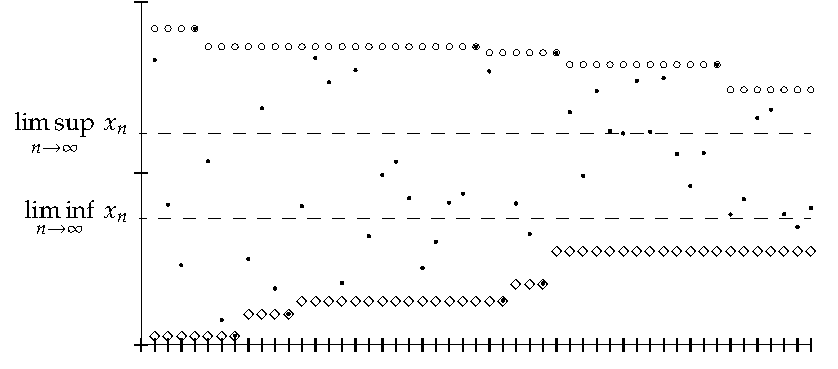
\includegraphics{figures/sequence-limsupliminf_an_bn}
\caption{First 50 terms of an example sequence.  Terms $x_n$ of the sequence are
marked with dots
%mbxSTARTIGNORE
(\raisebox{0.25ex}{\tiny$\bullet$}),
%mbxENDIGNORE
%mbxlatex ($\boldsymbol{\cdot}$),
$a_n$ are marked with
circles ($\circ$), and
$b_n$ are marked with diamonds ($\diamond$).\label{sequence-limsupliminf_an_bn}}
\end{myfigureht}

\begin{example} \label{example:liminfsupex}
Let $\{ x_n \}_{n=1}^\infty$ be defined by
\begin{equation*}
x_n \coloneqq
\begin{cases}
\frac{n+1}{n} & \text{if } n \text{ is odd,} \\
0             & \text{if } n \text{ is even.}
\end{cases}
\end{equation*}
Let us compute the $\liminf$ and $\limsup$ of this sequence.  See also
\figureref{sequence-limsupliminf_an_bn-example}.  First the
limit inferior:
\begin{equation*}
\liminf_{n\to\infty} x_n = 
\lim_{n\to\infty}
\bigl(
\inf \{ x_k : k \geq n \}
\bigr)
=
\lim_{n\to\infty} 0 = 0 .
\end{equation*}
For the limit superior, we write
\begin{equation*}
\limsup_{n\to\infty} x_n = 
\lim_{n\to\infty}
\bigl(
\sup \{ x_k : k \geq n \}
\bigr) .
\end{equation*}
It is not hard to see that
\begin{equation*}
\sup \{ x_k : k \geq n \} =
\begin{cases}
\frac{n+1}{n}   & \text{if } n \text{ is odd,} \\
\frac{n+2}{n+1} & \text{if } n \text{ is even.}
\end{cases}
\end{equation*}
We leave it to the reader to show that the limit is 1.  That is,
\begin{equation*}
\limsup_{n\to\infty} x_n = 1 .
\end{equation*}
Do note that the sequence $\{ x_n \}_{n=1}^\infty$ is not a convergent sequence.
\begin{myfigureht}
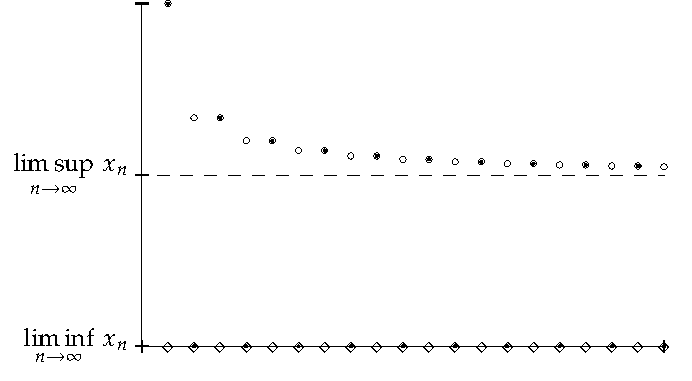
\includegraphics{figures/sequence-limsupliminf_an_bn-example}
\caption{First 20 terms of the sequence in \exampleref{example:liminfsupex}.
The marking is as in \figureref{sequence-limsupliminf_an_bn}.
\label{sequence-limsupliminf_an_bn-example}}
\end{myfigureht}
\end{example}

We associate certain subsequences with $\limsup$ and $\liminf$.
It is important to notice that $\{ a_n \}_{n=1}^\infty$ and
$\{ b_n \}_{n=1}^\infty$ are not
subsequences of $\{ x_n \}_{n=1}^\infty$, nor do they have to even 
consist of the same numbers.
For example, for the sequence $\{ \nicefrac{1}{n} \}_{n=1}^\infty$,
$b_n = 0$ for all $n \in \N$.

\begin{thm} \label{subseqlimsupinf:thm}
If $\{ x_n \}_{n=1}^\infty$ is a bounded sequence, then there exists a subsequence
$\{ x_{n_k} \}_{k=1}^\infty$ such that
\begin{equation*}
\lim_{k\to \infty} x_{n_k} = \limsup_{n \to \infty} x_n .
\end{equation*}
Similarly, there exists a (perhaps different) subsequence
$\{ x_{m_k} \}_{k=1}^\infty$ such that
\begin{equation*}
\lim_{k\to \infty} x_{m_k} = \liminf_{n \to \infty} x_n .
\end{equation*}
\end{thm}

\begin{proof}
Define $a_n \coloneqq \sup \{ x_k : k \geq n \}$.
Write
$x \coloneqq \limsup_{n\to\infty} x_n = \lim_{n\to\infty} a_n$.
We define the subsequence inductively.
Let $n_1 \coloneqq 1$, and suppose $n_1,n_2,\ldots,n_{k-1}$ are already defined for
some $k \geq 2$.  Pick an $m \geq n_{k-1} + 1$
such that
\begin{equation*}
a_{(n_{k-1}+1)} - x_m < \frac{1}{k} .
\end{equation*}
Such an $m$ exists
as $a_{(n_{k-1}+1)}$ is a supremum of the
set $\{ x_\ell : \ell \geq n_{k-1} + 1 \}$ and hence there are elements
of the sequence arbitrarily close (or even possibly equal) to the supremum.
Set $n_{k} \coloneqq  m$.  The subsequence $\{ x_{n_k} \}_{k=1}^\infty$ is defined.  Next, we
must prove that it converges to $x$.

For all $k \geq 2$, we have
$a_{(n_{k-1}+1)} \geq a_{n_k}$ (why?) and $a_{n_{k}} \geq x_{n_k}$.
Therefore, for every $k \geq 2$,
\begin{equation*}
\begin{split}
\abs{a_{n_k} - x_{n_k}} & = 
a_{n_k} - x_{n_k}
\\
& \leq
a_{(n_{k-1}+1)} - x_{n_k}
\\
& < \frac{1}{k} .
\end{split}
\end{equation*}

Let us show that $\{ x_{n_k} \}_{k=1}^\infty$ converges to $x$.
Note that the subsequence need not be monotone.  Let $\epsilon > 0$ be given.
As $\{ a_n \}_{n=1}^\infty$ converges to $x$, the subsequence
$\{ a_{n_k} \}_{k=1}^\infty$ converges to $x$.
Thus there exists an $M_1 \in \N$
such that for all $k \geq M_1$, we have
\begin{equation*}
\abs{a_{n_k} - x} < \frac{\epsilon}{2} .
\end{equation*}
Find an $M_2 \in \N$ such that
\begin{equation*}
\frac{1}{M_2} \leq \frac{\epsilon}{2}.
\end{equation*}
Take $M \coloneqq \max \{M_1 , M_2 , 2 \}$.  For all $k \geq M$,
\begin{equation*}
\begin{split}
\abs{x- x_{n_k}} & =
\abs{a_{n_k} - x_{n_k} + x - a_{n_k}}
\\
& \leq \abs{a_{n_k} - x_{n_k}} + \abs{x - a_{n_k}}
\\
& < \frac{1}{k} + \frac{\epsilon}{2}
\\
& \leq \frac{1}{M_2} + \frac{\epsilon}{2} \leq \frac{\epsilon}{2} +
\frac{\epsilon}{2} = \epsilon .
\end{split}
\end{equation*}

We leave the statement for $\liminf$ as an exercise.
\end{proof}

\subsection{Using limit inferior and limit superior}

The advantage of $\liminf$ and $\limsup$ is that we can always write them
down for any (bounded) sequence.
If we could somehow compute them, we could also compute the limit of the
sequence if it exists, or show that the sequence diverges.
Working with $\liminf$ and $\limsup$ is a
little bit like working with limits, although there are subtle differences.

\begin{prop} \label{liminfsupconv:prop}
Let $\{ x_n \}_{n=1}^\infty$ be a bounded sequence.  Then
$\{ x_n \}_{n=1}^\infty$ converges
if and only if
\begin{equation*}
\liminf_{n\to \infty} x_n = 
\limsup_{n\to \infty} x_n.
\end{equation*}
Furthermore, if $\{ x_n \}_{n=1}^\infty$ converges, then
\begin{equation*}
\lim_{n\to \infty} x_n = 
\liminf_{n\to \infty} x_n = 
\limsup_{n\to \infty} x_n.
\end{equation*}
\end{prop}

\begin{proof}
Let $a_n$ and $b_n$ be as in \defnref{liminflimsup:def}.
In particular, for all $n \in \N$,
\begin{equation*}
b_n \leq x_n \leq a_n .
\end{equation*}
First suppose
$\liminf_{n\to\infty} x_n = \limsup_{n\to\infty} x_n$.
Then $\{ a_n \}_{n=1}^\infty$ and $\{ b_n \}_{n=1}^\infty$
both converge to the same limit.
By the squeeze lemma
(\lemmaref{squeeze:lemma}), $\{ x_n \}_{n=1}^\infty$ converges and
\begin{equation*}
\lim_{n\to \infty} b_n
=
\lim_{n\to \infty} x_n
=
\lim_{n\to \infty} a_n .
\end{equation*}

Now suppose $\{ x_n \}_{n=1}^\infty$ converges to $x$.
By \thmref{subseqlimsupinf:thm},
there exists a subsequence $\{ x_{n_k} \}_{k=1}^\infty$
converging to $\limsup_{n\to\infty} x_n$.
As $\{ x_n \}_{n=1}^\infty$ converges to $x$,
every subsequence converges to $x$ and
so $\limsup_{n\to\infty} x_n = \lim_{k\to\infty} x_{n_k} = x$.
Similarly, $\liminf_{n\to\infty} x_n = x$.
\end{proof}

Limit superior and limit inferior behave nicely
with subsequences.

\begin{prop} \label{prop:subseqslimsupinf}
Suppose $\{ x_n \}_{n=1}^\infty$ is a bounded sequence and
$\{ x_{n_k} \}_{k=1}^\infty$ is a subsequence.  Then
\begin{equation*}
\liminf_{n\to\infty} x_n \leq
\liminf_{k\to\infty} x_{n_k} \leq
\limsup_{k\to\infty} x_{n_k} \leq
\limsup_{n\to\infty} x_n .
\end{equation*}
\end{prop}

\begin{proof}
The middle inequality has been proved already.  We will prove the third
inequality, and leave the first inequality as an exercise.

We want to prove that
$\limsup_{k\to\infty} x_{n_k} \leq \limsup_{n\to\infty} x_n$.  Define
$a_n \coloneqq \sup \{ x_k : k \geq n \}$ 
as usual.
Also define
$c_n \coloneqq \sup \{ x_{n_k} : k \geq n \}$.
It is not true that $\{ c_n \}_{n=1}^\infty$ is necessarily a subsequence
of $\{ a_n \}_{n=1}^\infty$.
However, as $n_k \geq k$ for all $k$, we have
$\{ x_{n_k} : k \geq n \} \subset \{ x_k : k \geq n \}$.
A supremum of a subset is less than or equal to the supremum of the
set, and therefore
\begin{equation*}
c_n \leq a_n \qquad \text{for all $n$}.
\end{equation*}
\lemmaref{limandineq:lemma} gives
\begin{equation*}
\lim_{n\to\infty} c_n \leq \lim_{n\to\infty} a_n ,
\end{equation*}
which is the desired conclusion.
\end{proof}

Limit superior and limit inferior
are the largest and smallest
subsequential limits.  If the subsequence $\{ x_{n_k} \}_{k=1}^\infty$ in the previous
proposition is convergent, then
$\liminf_{k\to\infty} x_{n_k} = \lim_{k\to\infty} x_{n_k} =
\limsup_{k\to\infty} x_{n_k}$.  Therefore,
\begin{equation*}
\liminf_{n\to\infty} x_n \leq
\lim_{k\to\infty} x_{n_k} \leq
\limsup_{n\to\infty} x_n .
\end{equation*}

Similarly, we get the following useful test for convergence
of a bounded sequence.  We leave the proof as an exercise.

\begin{prop} \label{seqconvsubseqconv:prop}
A bounded sequence $\{ x_n \}_{n=1}^\infty$ is convergent and converges to $x$
if and only if
every convergent subsequence
$\{ x_{n_k} \}_{k=1}^\infty$ converges to $x$.
\end{prop}

\subsection{Bolzano--Weierstrass theorem}

While it is not true that a bounded sequence is convergent, the
Bolzano--Weierstrass theorem tells us that we can at least find a convergent
subsequence.
The version of Bolzano--Weierstrass 
that we present in this section is the Bolzano--Weierstrass for
sequences of real numbers.

\begin{thm}[Bolzano--Weierstrass]\index{Bolzano--Weierstrass theorem}\label{thm:bwseq}
Suppose a sequence $\{ x_n \}_{n=1}^\infty$ of real numbers is bounded.
Then there exists a convergent subsequence $\{ x_{n_i} \}_{i=1}^\infty$.
\end{thm}

\begin{proof}
We use \thmref{subseqlimsupinf:thm}.  It says that there exists
a subsequence whose limit is $\limsup_{n\to\infty} x_n$.
\end{proof}

The reader might complain right now that 
\thmref{subseqlimsupinf:thm} is strictly stronger than the
Bolzano--Weierstrass theorem as presented above.  That is true.
However, 
\thmref{subseqlimsupinf:thm} only applies to the real line, but
Bolzano--Weierstrass applies in more general contexts (that is, in $\R^n$)
with pretty much the exact same statement.

As the theorem is so important to analysis, we present an explicit
proof.
The idea of the following proof also generalizes to different contexts.

\begin{proof}[Alternate proof of Bolzano--Weierstrass]
As the sequence is bounded, then there exist two numbers $a_1 < b_1$
such that $a_1 \leq x_n \leq b_1$ for all $n \in \N$.
We will define a subsequence $\{ x_{n_i} \}_{i=1}^\infty$ and two
sequences $\{ a_i \}_{i=1}^\infty$ and $\{ b_i \}_{i=1}^\infty$, such that
$\{ a_i \}_{i=1}^\infty$ is monotone increasing, $\{ b_i \}_{i=1}^\infty$ is monotone decreasing,
$a_i \leq x_{n_i} \leq b_i$ and such that $\lim_{i\to\infty} a_i =
\lim_{i\to\infty} b_i$.   That
$x_{n_i}$ converges then follows by the \hyperref[squeeze:lemma]{squeeze lemma}.

We define the sequences inductively.  We will define the sequences so that
for all $i$, we have $a_i < b_i$,
and that $x_n \in [a_i,b_i]$ for infinitely many $n \in \N$.
We have already defined $a_1$ and $b_1$.  We take $n_1 \coloneqq 1$, that is
$x_{n_1} = x_1$.
Suppose that up to some $k \in \N$,
we have defined the subsequence $x_{n_1}, x_{n_2}, \ldots,
x_{n_k}$, and the sequences $a_1,a_2,\ldots,a_k$
and $b_1,b_2,\ldots,b_k$.
Let $y \coloneqq \frac{a_k+b_k}{2}$.
Clearly
$a_k < y < b_k$.  If there exist infinitely many $j \in \N$
such that $x_j \in [a_k,y]$, then set $a_{k+1} \coloneqq a_k$, $b_{k+1}
\coloneqq y$,
and pick $n_{k+1} > n_{k}$
such that $x_{n_{k+1}} \in [a_k,y]$.  If there are not infinitely many 
$j$ such that 
$x_j \in [a_k,y]$, then it must be true that there are infinitely many $j \in
\N$ such that 
$x_j \in [y,b_k]$.  In this case pick $a_{k+1} \coloneqq y$, $b_{k+1}
\coloneqq b_k$,
and pick $n_{k+1} > n_{k}$
such that $x_{n_{k+1}} \in [y,b_k]$.

We now have the sequences defined.  What is left to prove is that
$\lim_{i\to\infty} a_i = \lim_{i\to\infty} b_i$.  The limits exist as the sequences
are monotone.  In the construction,
$b_i - a_i$ is cut in half in each step.  Therefore,
$b_{i+1} - a_{i+1} = \frac{b_i-a_i}{2}$.  By
\hyperref[induction:thm]{induction},
\begin{equation*}
b_i - a_i = \frac{b_1-a_1}{2^{i-1}} .
\end{equation*}

Let $x \coloneqq \lim_{i\to\infty} a_i$.  As $\{ a_i \}_{i=1}^\infty$ is monotone,
\begin{equation*}
x = \sup \{ a_i : i \in \N \} .
\end{equation*}
Let $y \coloneqq \lim_{i\to\infty} b_i = \inf \{ b_i : i \in \N \}$.  Since $a_i < b_i$ for
all $i$, then $x \leq y$.
As the sequences are monotone, then
for all $i$, we have (why?)
\begin{equation*}
y-x \leq b_i-a_i = \frac{b_1-a_1}{2^{i-1}} .
\end{equation*}
Because $\frac{b_1-a_1}{2^{i-1}}$ is arbitrarily small and $y-x \geq 0$,
we have $y-x = 0$.  Finish by the \hyperref[squeeze:lemma]{squeeze lemma}.
\end{proof}

Yet another proof of the Bolzano--Weierstrass theorem is to show the
following claim,
which is left as a challenging exercise.
\emph{Claim: Every sequence has a monotone subsequence}.

\subsection{Infinite limits}

Just as for infima and suprema, it is possible to allow certain
limits to be infinite.  That is, we write $\lim_{n\to\infty} x_n = \infty$ or
$\lim_{n\to\infty} x_n = -\infty$ for certain divergent sequences.

\begin{defn}
\index{infinite limit!of a sequence}\index{limit!infinite}
We say
$\{ x_n \}_{n=1}^\infty$ \emph{\myindex{diverges to infinity}}%
\footnote{Sometimes it is said that $\{ x_n \}_{n=1}^\infty$ \emph{converges to infinity}.}
if for every $K \in
\R$, there exists an $M \in \N$ such that for all $n \geq M$, we have $x_n >
K$.  In this case we write
\begin{equation*}
\lim_{n \to \infty} x_n \coloneqq \infty .  
\end{equation*}
Similarly,
if for every $K \in \R$ there exists an $M \in \N$ such that
for all $n \geq M$, we have $x_n < K$, we say $\{ x_n \}_{n=1}^\infty$
\emph{\myindex{diverges to minus infinity}} and we write
\begin{equation*}
\lim_{n \to \infty} x_n \coloneqq -\infty .  
\end{equation*}
\end{defn}

With this definition and allowing $\infty$ and $-\infty$,
we can write $\lim_{n\to\infty} x_n$ for any monotone sequence.

\begin{prop} \label{prop:unboundedmonotone}
Suppose $\{ x_n \}_{n=1}^\infty$ is a monotone unbounded sequence.  Then
\begin{equation*}
\lim_{n \to \infty} x_n =
\begin{cases}
\infty  & \text{if } \{ x_n \}_{n=1}^\infty \text{ is increasing,} \\
-\infty & \text{if } \{ x_n \}_{n=1}^\infty \text{ is decreasing.}
\end{cases}
\end{equation*}
\end{prop}

\begin{proof}
The case of monotone increasing follows from
\exerciseref{exercise:infseqlimlims} part c) below.
Suppose $\{x_n\}_{n=1}^\infty$ is decreasing and unbounded.
That the sequence is unbounded means that
for every $K \in \R$, there is an $M \in \N$ such that $x_M < K$.
By monotonicity, $x_n \leq x_M < K$ for all $n \geq M$.
Therefore, $\lim_{n\to\infty} x_n = -\infty$.
\end{proof}

\begin{example}
\begin{equation*}
\lim_{n\to \infty} n = \infty,
\qquad
\lim_{n\to \infty} n^2 = \infty,
\qquad
\lim_{n\to \infty} -n = -\infty.
\end{equation*}
We leave verification to the reader.
\end{example}

We may also allow $\liminf$ and $\limsup$ to take on
the values $\infty$ and $-\infty$, so that
we can apply $\liminf$ and $\limsup$
to absolutely any sequence, not just
a bounded one.   Unfortunately, the sequences $\{ a_n \}_{n=1}^\infty$ and
$\{ b_n \}_{n=1}^\infty$
are not sequences of real numbers but of extended real numbers.  In
particular, $a_n$ can equal $\infty$ for some $n$, and $b_n$ can equal
$-\infty$.  So we have no definition for the limits.
But since the extended real numbers are still an ordered set, we
can take suprema and infima.

\begin{defn}
Let $\{ x_n \}_{n=1}^\infty$ be an unbounded sequence of real numbers.  Define
sequences of extended real numbers by
$a_n \coloneqq \sup \{ x_k : k \geq n \}$ and
$b_n \coloneqq \inf \{ x_k : k \geq n \}$.
Define\glsadd{not:limsupseq}\glsadd{not:liminfseq}
\index{limit inferior}\index{limit superior}\index{limsup}\index{liminf}
\begin{equation*}
\limsup_{n \to \infty} x_n \coloneqq \inf \{ a_n : n \in \N \}, \qquad \text{and} \qquad
\liminf_{n \to \infty} x_n \coloneqq \sup \{ b_n : n \in \N \}.
\end{equation*}
\end{defn}

This definition agrees with the definition for bounded
sequences whenever $\lim_{n\to\infty} a_n$ or $\lim_{n\to\infty} b_n$ makes sense including
possibly $\infty$ and $-\infty$.

\begin{prop}
Let $\{ x_n \}_{n=1}^\infty$ be an unbounded sequence.  Define
$\{ a_n \}_{n=1}^\infty$ and $\{ b_n \}_{n=1}^\infty$ as above.
Then $\{ a_n \}_{n=1}^\infty$ is decreasing, and $\{ b_n \}_{n=1}^\infty$ is increasing.
If $a_n$ is a real number for every $n$, then
$\limsup_{n\to\infty} x_n = \lim_{n\to\infty} a_n$.
If $b_n$ is a real number for every $n$, then
$\liminf_{n\to\infty} x_n = \lim_{n\to\infty} b_n$.
\end{prop}

\begin{proof}
As before,
$a_n = \sup \{ x_k : k \geq n \} \geq \sup \{ x_k : k \geq n+1 \} =
a_{n+1}$.  So $\{ a_n \}_{n=1}^\infty$ is decreasing. Similarly,
$\{ b_n \}_{n=1}^\infty$ is increasing.

If the sequence $\{ a_n \}_{n=1}^\infty$ is a sequence of real numbers, then
$\lim_{n\to\infty} a_n = \inf \{ a_n : n \in \N \}$.  This follows from
\propref{prop:monotoneconv} if $\{ a_n \}_{n=1}^\infty$ is bounded and
\propref{prop:unboundedmonotone} if $\{a_n \}_{n=1}^\infty$
is unbounded.  We proceed similarly with $\{ b_n \}_{n=1}^\infty$.
\end{proof}

The definition behaves as expected with
$\limsup$ and $\liminf$, see exercises \ref{exercise:infseqlimex}
and \ref{exercise:infseqlimlims}.

\begin{example}
Suppose
$x_n \coloneqq 0$ for odd $n$ and $x_n \coloneqq n$ for even $n$.
Then $a_n = \infty$ for all $n$, since for every $M$,
there exists an even $k$ such that $x_k = k \geq M$.
On the other hand, $b_n = 0$ for all $n$, as
for every $n$, the set
$\{ b_k : k \geq n \}$ consists of $0$ and positive numbers.
So,
\begin{equation*}
\lim_{n\to \infty} x_n \quad \text{does not exist},
\qquad
\limsup_{n\to \infty} x_n = \infty ,
\qquad
\liminf_{n\to \infty} x_n = 0.
\end{equation*}
\end{example}

\subsection{Exercises}

\begin{exercise}
Suppose $\{ x_n \}_{n=1}^\infty$ is a bounded sequence.  Define $a_n$ and
$b_n$ as in \defnref{liminflimsup:def}.  Show that $\{ a_n \}_{n=1}^\infty$
and $\{ b_n \}_{n=1}^\infty$ are bounded.
\end{exercise}

\begin{exercise}
Suppose $\{ x_n \}_{n=1}^\infty$ is a bounded sequence.
Define $b_n$ as in \defnref{liminflimsup:def}.  Show that
$\{ b_n \}_{n=1}^\infty$ is an increasing sequence.
\end{exercise}

\begin{exercise}
Finish the proof of \propref{prop:subseqslimsupinf}.  That is,
suppose $\{ x_n \}_{n=1}^\infty$ is a bounded sequence and
$\{ x_{n_k} \}_{k=1}^\infty$ is a subsequence.  Prove
$\displaystyle \liminf_{n\to\infty} x_n \leq
\liminf_{k\to\infty} x_{n_k}$.
\end{exercise}

\begin{exercise}
Prove \propref{seqconvsubseqconv:prop}.
\end{exercise}

\begin{exercise}
\leavevmode
\begin{enumerate}[a)]
\item
Let $x_n \coloneqq \dfrac{{(-1)}^n}{n}$.
Find $\limsup\limits_{n\to\infty} x_n$ and $\liminf\limits_{n\to\infty} x_n$.
\item
Let $x_n \coloneqq \dfrac{(n-1){(-1)}^n}{n}$.
Find $\limsup\limits_{n\to\infty} x_n$ and $\liminf\limits_{n\to\infty} x_n$.
\end{enumerate}
\end{exercise}

\begin{exercise}
Let $\{ x_n \}_{n=1}^\infty$ and $\{ y_n \}_{n=1}^\infty$ be bounded sequences such that
$x_n \leq y_n$ for all $n$.  Show
\begin{equation*}
\limsup_{n\to\infty} x_n \leq
\limsup_{n\to\infty} y_n
\qquad \text{and} \qquad
\liminf_{n\to\infty} x_n \leq
\liminf_{n\to\infty} y_n .
\end{equation*}
\end{exercise}

\begin{exercise}
Let $\{ x_n \}_{n=1}^\infty$ and $\{ y_n \}_{n=1}^\infty$ be bounded sequences.
\begin{enumerate}[a)]
\item
Show that $\{ x_n + y_n \}_{n=1}^\infty$ is bounded.
\item
Show that
\begin{equation*}
\Bigl(\liminf_{n\to \infty} x_n\Bigr)
+
\Bigl(\liminf_{n\to \infty} y_n\Bigr)
\leq
\liminf_{n\to \infty} \, (x_n+y_n) .
\end{equation*}
Hint: One proof is to find a subsequence $\{ x_{n_m}+y_{n_m} \}_{m=1}^\infty$ of
$\{ x_n + y_n \}_{n=1}^\infty$ that converges.
Then find a subsequence $\{ x_{n_{m_i}} \}_{i=1}^\infty$ of
$\{ x_{n_m} \}_{m=1}^\infty$ that converges.
\item
Find an explicit $\{ x_n \}_{n=1}^\infty$ and $\{ y_n \}_{n=1}^\infty$ such that
\begin{equation*}
\Bigl(\liminf_{n\to \infty} x_n\Bigr)
+
\Bigl(\liminf_{n\to \infty} y_n\Bigr)
<
\liminf_{n\to \infty} \, (x_n+y_n) .
\end{equation*}
Hint: Look for examples that do not have a limit.
\end{enumerate}
\end{exercise}

\begin{samepage}
\begin{exercise}
Let $\{ x_n \}_{n=1}^\infty$ and $\{ y_n \}_{n=1}^\infty$ be bounded sequences (by the previous
exercise, $\{ x_n + y_n \}_{n=1}^\infty$ is bounded).
\begin{enumerate}[a)]
\item
Show that
\begin{equation*}
\Bigl(\limsup_{n\to \infty} x_n\Bigr)
+
\Bigl(\limsup_{n\to \infty} y_n\Bigr)
\geq
\limsup_{n\to \infty} \, (x_n+y_n) .
\end{equation*}
Hint: See previous exercise.
\item
Find an explicit $\{ x_n \}_{n=1}^\infty$ and $\{ y_n \}_{n=1}^\infty$ such that
\begin{equation*}
\Bigl(\limsup_{n\to \infty} x_n\Bigr)
+
\Bigl(\limsup_{n\to \infty} y_n\Bigr)
>
\limsup_{n\to \infty} \, (x_n+y_n) .
\end{equation*}
Hint: See previous exercise.
\end{enumerate}
\end{exercise}
\end{samepage}

\begin{exercise}
If $S \subset \R$ is a set, then $x \in \R$ is a \emph{\myindex{cluster
point}}
if for every $\epsilon > 0$, the set $(x-\epsilon,x+\epsilon) \cap S
\setminus \{ x \}$ is not empty.  That is, if there are points of $S$
arbitrarily close to $x$.
For example, $S \coloneqq \{ \nicefrac{1}{n} : n \in \N \}$ has a unique (only
one) cluster point $0$, but $0 \notin S$.
Prove the following version of the Bolzano--Weierstrass theorem:

\medskip

\noindent
\emph{\textbf{Theorem.} Let $S \subset \R$ be a bounded infinite set,
then there exists at least one cluster point of $S$}.

\medskip

Hint: If $S$ is infinite, then $S$ contains a countably infinite subset.
That is, there is a sequence $\{ x_n \}_{n=1}^\infty$ of distinct numbers in $S$.
\end{exercise}

\begin{samepage}
\begin{exercise}[Challenging]
\leavevmode
\begin{enumerate}[a)]
\item
Prove that every sequence contains a monotone subsequence.
Hint: Call $n \in \N$ a \emph{peak} if $a_m \leq a_n$ for all $m \geq n$.
There are two possibilities: Either the sequence has at most finitely many
peaks,
or it has infinitely many peaks.
\item
Conclude the Bolzano--Weierstrass theorem.
\end{enumerate}
\end{exercise}
\end{samepage}

\begin{exercise}
Prove a stronger version of \propref{seqconvsubseqconv:prop}.
Suppose $\{ x_n \}_{n=1}^\infty$ is a sequence such that every subsequence
$\{ x_{n_m} \}_{m=1}^\infty$ has a subsequence
$\{ x_{n_{m_i}} \}_{i=1}^\infty$ that converges to $x$.
\begin{enumerate}[a)]
\item
First show that $\{ x_n \}_{n=1}^\infty$ is
bounded.
\item
Now show that $\{ x_n \}_{n=1}^\infty$ converges to $x$.
\end{enumerate}
\end{exercise}

\begin{exercise}
Let $\{x_n\}_{n=1}^\infty$ be a bounded sequence.
\begin{enumerate}[a)]
\item
Prove that there exists an $s$ such that for every $r > s$, there exists 
an $M \in \N$ such that for all $n \geq M$, we have
$x_n < r$.
\item
If $s$ is a number as in a), then prove $\limsup\limits_{n\to\infty} x_n \leq s$.
\item
Show that if $S$ is the set of all $s$ as in a), then
$\limsup\limits_{n\to\infty} x_n = \inf \, S$.
\end{enumerate}
\end{exercise}

\begin{exercise}[Easy] \label{exercise:infseqlimex}
\pagebreak[2]
Suppose $\{ x_n \}_{n=1}^\infty$ is such that $\liminf\limits_{n\to\infty} x_n = -\infty$,
$\limsup\limits_{n\to\infty} x_n = \infty$.
\begin{enumerate}[a)]
\item
Show that $\{ x_n \}_{n=1}^\infty$ is not convergent, and also
that neither $\lim\limits_{n\to\infty} x_n = \infty$
nor $\lim\limits_{n\to\infty} x_n = -\infty$
is true.
\item
Find an example of such a sequence.
\end{enumerate}
\end{exercise}

\begin{exercise} \label{exercise:infseqlimlims}
Let $\{ x_n \}_{n=1}^\infty$ be a sequence.
\begin{enumerate}[a)]
\item
Show that
$\lim\limits_{n\to\infty} x_n = \infty$ if and only if
$\liminf\limits_{n\to\infty} x_n = \infty$.
\item
Then show that $\lim\limits_{n\to\infty} x_n = - \infty$ if and only if
$\limsup\limits_{n\to\infty} x_n = -\infty$.
\item
If $\{ x_n \}_{n=1}^\infty$ is monotone increasing, show that either
$\lim_{n\to\infty} x_n$ exists and is finite or $\lim_{n\to\infty} x_n = \infty$.  In either
case, $\lim_{n\to\infty} x_n = \sup \{ x_n : n \in \N \}$.
\end{enumerate}
\end{exercise}

\begin{exercise} \label{exercise:strongerratiotest2}
Prove the following stronger version of \lemmaref{seq:ratiotest}, the ratio
test.
Suppose $\{ x_n \}_{n=1}^\infty$ is a sequence such that $x_n \not= 0$ for all
$n$.
\begin{enumerate}[a)]
\item
Prove that if
\begin{equation*}
\limsup_{n \to \infty} \frac{\abs{x_{n+1}}}{\abs{x_n}} < 1 ,
\end{equation*}
then $\{ x_n \}_{n=1}^\infty$ converges to $0$.
\item
Prove that if
\begin{equation*}
\liminf_{n \to \infty} \frac{\abs{x_{n+1}}}{\abs{x_n}} > 1 ,
\end{equation*}
then $\{ x_n \}_{n=1}^\infty$ is unbounded.
\end{enumerate}
\end{exercise}

\begin{exercise}
Suppose $\{ x_n \}_{n=1}^\infty$ is a bounded sequence, $a_n \coloneqq \sup \{ x_k : k \geq n \}$
as before.  Suppose that for some $\ell \in \N$,
$a_\ell \notin \{ x_k : k \geq \ell \}$.  Then show that $a_j = a_\ell$ for all $j \geq \ell$, and hence
$\limsup\limits_{n\to\infty} x_n = a_\ell$.
\end{exercise}

\begin{exercise}
Suppose $\{ x_n \}_{n=1}^\infty$ is a sequence,
and $a_n \coloneqq \sup \{ x_k : k \geq n \}$ and
$b_n \coloneqq \sup \{ x_k : k \geq n \}$ as before.
\begin{enumerate}[a)]
\item
Prove that if $a_\ell = \infty$ for some $\ell \in \N$, then 
$\limsup\limits_{n\to\infty} x_n = \infty$.
\item
Prove that if $b_\ell = -\infty$ for some $\ell \in \N$, then 
$\liminf\limits_{n\to\infty} x_n = -\infty$.
\end{enumerate}
\end{exercise}

\begin{exercise}
Suppose $\{ x_n \}_{n=1}^\infty$ is a sequence
such that both $\liminf_{n\to\infty} x_n$ and
$\limsup_{n\to\infty} x_n$  are finite.  Prove that $\{ x_n \}_{n=1}^\infty$ is bounded.
\end{exercise}

\begin{exercise}
Suppose $\{ x_n \}_{n=1}^\infty$ is a bounded sequence, and $\epsilon > 0$ is given.
Prove that there exists an $M$ such that for all $k \geq M$,
\begin{equation*}
x_k - \Bigl(\limsup_{n\to\infty} x_n\Bigr) < \epsilon \qquad \text{and} \qquad
\Bigl(\liminf_{n\to\infty} x_n\Bigr) - x_k < \epsilon .
\end{equation*}
\end{exercise}

\begin{exercise} \label{exercise:extendsubseqlimsupinf}
Extend \thmref{subseqlimsupinf:thm} to unbounded sequences:
Suppose that $\{ x_n \}_{n=1}^\infty$ is a sequence.
If $\limsup_{n\to\infty} x_n = \infty$, then prove that
there exists a subsequence $\{ x_{n_i} \}_{i=1}^\infty$ converging to $\infty$.
Then prove the same result for $-\infty$, and then prove both statements for
$\liminf$.
\end{exercise}


%%%%%%%%%%%%%%%%%%%%%%%%%%%%%%%%%%%%%%%%%%%%%%%%%%%%%%%%%%%%%%%%%%%%%%%%%%%%%%

\sectionnewpage
\section{Cauchy sequences}
\label{sec:cauchy}

\sectionnotes{less than a lecture}

Often we wish to describe a certain number 
by a sequence that converges to it.  In this case, it is impossible to use the
number itself in the proof that the sequence converges.
It would be nice if we could check for convergence without knowing
the limit.

\begin{defn}
A sequence $\{ x_n \}_{n=1}^\infty$ is a \emph{\myindex{Cauchy sequence}}%
\footnote{%
Named after the French mathematician
\href{https://en.wikipedia.org/wiki/Cauchy}{Augustin-Louis Cauchy} (1789--1857).} if
for every $\epsilon > 0$ there exists an $M \in \N$ such that
for all $n \geq M$ and all $k \geq M$, we have
\begin{equation*}
\abs{x_n - x_k} < \epsilon .
\end{equation*}
\end{defn}

Informally, being Cauchy means that the terms of the sequence are eventually
all arbitrarily close to each other.  We might expect such a sequence to be
convergent, and we would be correct due to $\R$ having the
\hyperref[defn:lub]{least-upper-bound property}.  Before we prove this fact,
we look at some examples.

\begin{example}
The sequence $\{ \nicefrac{1}{n} \}_{n=1}^\infty$ is a Cauchy sequence.

Proof:  Given $\epsilon > 0$, find $M$ such that
$M > \nicefrac{2}{\epsilon}$.  Then for $n,k \geq M$,
we have $\nicefrac{1}{n} < \nicefrac{\epsilon}{2}$
and
$\nicefrac{1}{k} < \nicefrac{\epsilon}{2}$.  Therefore, for $n, k \geq M$,
we have
\begin{equation*}
\abs{\frac{1}{n} - \frac{1}{k}}
\leq
\abs{\frac{1}{n}} + \abs{\frac{1}{k}}
< \frac{\epsilon}{2} + \frac{\epsilon}{2} = \epsilon.
\end{equation*}
\end{example}

\begin{example}
The sequence $\bigl\{ {(-1)}^n \bigr\}_{n=1}^\infty$ is not a Cauchy sequence.

Proof:
Given any $M \in \N$, take $n \geq M$ to be any even number, and
let $k \coloneqq n+1$.  Then
\begin{equation*}
\begin{split}
\abs{{(-1)}^n - {(-1)}^k}
& =
\abs{{(-1)}^n - {(-1)}^{n+1}}
\\
& =
\abs{1 - (-1)} = 2 .
\end{split}
\end{equation*}
Therefore, for any $\epsilon \leq 2$ the definition cannot be satisfied, and
the sequence is not Cauchy.
\end{example}

%\begin{example}
%The sequence $\{ \frac{n+1}{n} \}_{n=1}^\infty$ is a Cauchy sequence.
%
%Proof:  Given $\epsilon > 0$, find $M$ such that
%$M > \nicefrac{2}{\epsilon}$.  Then for $n,k \geq M$,
%we have $\nicefrac{1}{n} < \nicefrac{\epsilon}{2}$
%and
%$\nicefrac{1}{k} < \nicefrac{\epsilon}{2}$.  Therefore, for $n, k \geq M$,
%we have
%\begin{equation*}
%\begin{split}
%\abs{\frac{n+1}{n} - \frac{k+1}{k}}
%& =
%\abs{\frac{k(n+1)-n(k+1)}{nk}}
%\\
%& =
%\abs{\frac{kn+k-nk-n}{nk}}
%\\
%& =
%\abs{\frac{k-n}{nk}}
%\\
%& \leq
%\abs{\frac{k}{nk}}
%+
%\abs{\frac{-n}{nk}}
%\\
%& = \frac{1}{n} + \frac{1}{k}
%< \frac{\epsilon}{2} + \frac{\epsilon}{2} = \epsilon .
%\end{split}
%\end{equation*}
%\end{example}

\begin{prop}
If a sequence is Cauchy, then it is bounded.
\end{prop}

\begin{proof}
Suppose $\{ x_n \}_{n=1}^\infty$ is Cauchy.  Pick an $M$ such that for all
$n,k \geq M$, we have $\abs{x_n-x_k} < 1$.  In particular, 
for all $n \geq M$,
\begin{equation*}
\abs{x_n - x_M} < 1 .
\end{equation*}
By the reverse triangle inequality,
$\abs{x_n} - \abs{x_M} \leq \abs{x_n - x_M} < 1$.  Hence for $n \geq M$,
\begin{equation*}
\abs{x_n} < 1 + \abs{x_M}.
\end{equation*}
Let
\begin{equation*}
B \coloneqq \max \bigl\{ \abs{x_1}, \abs{x_2}, \ldots, \abs{x_{M-1}}, 1+ \abs{x_M} \bigr\} .
\end{equation*}
Then $\abs{x_n} \leq B$ for all $n \in \N$.
\end{proof}

\begin{thm}
A sequence of real numbers is Cauchy if and only if it converges.
\end{thm}

\begin{proof}
Suppose $\{ x_n \}_{n=1}^\infty$ converges to $x$,
and
let $\epsilon > 0$ be given.
Then there 
exists an $M$ such that for $n \geq M$,
\begin{equation*}
\abs{x_n - x} < \frac{\epsilon}{2} .
\end{equation*}
Hence for $n \geq M$ and $k \geq M$,
\begin{equation*}
\abs{x_n - x_k} = 
\abs{x_n - x + x - x_k}
\leq \abs{x_n-x} + \abs{x-x_k} < \frac{\epsilon}{2} + \frac{\epsilon}{2} =
\epsilon .
\end{equation*}

Alright, that direction was easy.  Now suppose $\{ x_n \}_{n=1}^\infty$ is Cauchy.
We have shown that $\{ x_n \}_{n=1}^\infty$ is bounded.
For a bounded sequence, liminf and limsup exist, and this is
where we use the
\hyperref[defn:lub]{least-upper-bound property}.
If we show that
\begin{equation*}
\liminf_{n\to \infty} x_n = \limsup_{n\to\infty} x_n ,
\end{equation*}
then $\{ x_n \}_{n=1}^\infty$ must be convergent by \propref{liminfsupconv:prop}.


Define $a \coloneqq \limsup_{n\to\infty} x_n$ and
$b \coloneqq \liminf_{n\to\infty} x_n$.
By \thmref{subseqlimsupinf:thm}, there exist subsequences
$\{ x_{n_i} \}_{i=1}^\infty$ and
$\{ x_{m_i} \}_{i=1}^\infty$, such that
\begin{equation*}
\lim_{i\to\infty} x_{n_i} = a
\qquad \text{and} \qquad
\lim_{i\to\infty} x_{m_i} = b.
\end{equation*}
Given an $\epsilon > 0$,
there exists an $M_1$ such that
$\abs{x_{n_i} - a} < \nicefrac{\epsilon}{3}$ for all $i \geq M_1$
and an $M_2$ such that
$\abs{x_{m_i} - b} < \nicefrac{\epsilon}{3}$ for all $i \geq M_2$.
There also exists an $M_3$
such that
$\abs{x_n-x_k} < \nicefrac{\epsilon}{3}$
for all $n,k \geq M_3$.
Let $M \coloneqq \max \{ M_1, M_2, M_3 \}$.
If $i \geq M$, then $n_i \geq M$ and $m_i \geq M$.  Hence,
\begin{equation*}
\begin{split}
\abs{a-b} & =
\abs{a-x_{n_i}+x_{n_i}
-x_{m_i}+x_{m_i}
-b} \\
& \leq
\abs{a-x_{n_i}}
+ \abs{x_{n_i} -x_{m_i}}
+ \abs{x_{m_i} -b} \\
& <
\frac{\epsilon}{3}
+
\frac{\epsilon}{3}
+
\frac{\epsilon}{3}
= \epsilon .
\end{split}
\end{equation*}
As $\abs{a-b} < \epsilon$ for all $\epsilon > 0$, then $a=b$ and 
the sequence converges.
\end{proof}

\begin{remark}
The statement of this theorem is sometimes used to define the
completeness property of the real numbers.  We say a set is
\emph{\myindex{Cauchy-complete}} (or sometimes just \emph{\myindex{complete}})
if every Cauchy sequence converges to something in the set.
Above, we proved that
as $\R$ has the \hyperref[defn:lub]{least-upper-bound property}, $\R$ is 
Cauchy-complete.
One can construct $\R$ via
\myquote{completing} $\Q$ by \myquote{throwing in} just enough points to make all
Cauchy sequences converge (we omit the details).
The resulting field has the
least-upper-bound property.
The advantage of defining completeness via Cauchy
sequences is that it generalizes to
more abstract settings such as metric spaces, see \chapterref{ms:chapter}.
\end{remark}

The Cauchy criterion is stronger than 
$\abs{x_{n+1}-x_n}$ (or $\abs{x_{n+j}-x_n}$ for a fixed $j$) going to zero as
$n$ goes to
infinity.  When we get to the partial sums of the harmonic series
(see \exampleref{example:harmonicseries} in the next section), we will have
a sequence such that $x_{n+1}-x_n = \nicefrac{1}{n}$,
yet $\{ x_n \}_{n=1}^\infty$ is divergent.
In fact, for that sequence,
$\lim_{n\to\infty} \abs{x_{n+j}-x_n} = 0$ for
every $j \in \N$ (compare \exerciseref{exercise:badnocauchy}).
The key point in the definition of Cauchy is that $n$ and $k$
vary independently and can be arbitrarily far apart.

\subsection{Exercises}

\begin{exercise}
Prove that $\{ \frac{n^2-1}{n^2} \}_{n=1}^\infty$ is Cauchy using directly the definition
of Cauchy sequences.
\end{exercise}

\begin{exercise}
Let $\{ x_n \}_{n=1}^\infty$ be a sequence such that
there exists a positive $C < 1$ and for all $n$,
\begin{equation*}
\abs{x_{n+1} - x_n} \leq C \abs{x_{n}-x_{n-1}} .
\end{equation*}
Prove that $\{ x_n \}_{n=1}^\infty$ is Cauchy.
Hint:  You can freely use the formula (for $C \not= 1$)
\begin{equation*}
1+ C+ C^2 + \cdots + C^n = \frac{1-C^{n+1}}{1-C}.
\end{equation*}
\end{exercise}

\begin{exercise}[Challenging]
Suppose $F$ is an ordered field that contains the rational numbers
$\Q$, such that $\Q$ is dense,
that is: Whenever $x,y \in F$ are such that $x < y$,
then there exists a $q \in \Q$ such that $x < q < y$.
Say a sequence $\{ x_n \}_{n=1}^\infty$ of rational numbers is Cauchy
if given every $\epsilon \in \Q$ with $\epsilon > 0$, there exists
an $M$ such that for all $n,k \geq M$, we have $\abs{x_n-x_k} < \epsilon$.
Suppose every Cauchy sequence of rational numbers has a limit in $F$.
Prove that $F$ has the \hyperref[defn:lub]{least-upper-bound property}.
\end{exercise}

\begin{exercise}
Let $\{ x_n \}_{n=1}^\infty$ and $\{ y_n \}_{n=1}^\infty$ be sequences such
that $\lim_{n\to\infty} y_n =0$.  Suppose that for all $k \in \N$
and
for all $m \geq k$, we have
\begin{equation*}
\abs{x_m-x_k} \leq y_k .
\end{equation*}
Show that $\{ x_n \}_{n=1}^\infty$ is Cauchy.
\end{exercise}

\begin{exercise}
Suppose a Cauchy sequence $\{ x_n \}_{n=1}^\infty$ is such that for every $M \in \N$,
there exists a $k \geq M$ and an $n \geq M$ such that
$x_k < 0$ and $x_n > 0$.  Using simply the definition of a Cauchy sequence
and of a convergent sequence, show that
the sequence converges to $0$.
\end{exercise}

\begin{exercise}
Suppose $\abs{x_n-x_k} \leq \nicefrac{n}{k^2}$ for all $n$ and $k$.
Show that $\{ x_n \}_{n=1}^\infty$ is Cauchy.
%\footnote{After proving that
%the sequence is Cauchy, for an extra exercise, prove the sequence is constant.}
\end{exercise}

\begin{exercise}
Suppose $\{ x_n \}_{n=1}^\infty$ is a Cauchy sequence such that for infinitely many
$n$, $x_n = c$.  Using only the definition of Cauchy sequence prove 
that $\lim\limits_{n\to\infty} x_n = c$.
\end{exercise}

\begin{exercise}
True or false, prove or find a counterexample:  If $\{ x_n \}_{n=1}^\infty$ is a Cauchy
sequence, then there exists an $M$
such that for all $n \geq M$, we have
$\abs{x_{n+1}-x_n}
\leq
\abs{x_{n}-x_{n-1}}$.
\end{exercise}


%%%%%%%%%%%%%%%%%%%%%%%%%%%%%%%%%%%%%%%%%%%%%%%%%%%%%%%%%%%%%%%%%%%%%%%%%%%%%%

\sectionnewpage
\section{Series}
\label{sec:series}

\sectionnotes{2 lectures}

A fundamental object in mathematics is that of a series.  In fact, when
the foundations of analysis were being developed, the motivation was to
understand series.  Understanding series is important in applications
of analysis.  For example, solutions to differential equations are often
given as series, and differential equations are the basis for understanding
almost all of modern science.

\subsection{Definition}

\begin{defn}
Given a sequence $\{ x_n \}_{n=1}^\infty$, we write the formal object
\begin{equation*}
\sum_{n=1}^\infty x_n
%\qquad
%\text{or sometimes just}
%\qquad
%\sum x_n
\end{equation*}
\glsadd{not:series}
and call it a \emph{\myindex{series}}.  A series
\emph{converges}\index{convergent!series} if the sequence
$\{ s_k \}_{k=1}^\infty$
defined by
\glsadd{not:finitesum}
\begin{equation*}
s_k \coloneqq \sum_{n=1}^k x_n = x_1 + x_2 + \cdots + x_k
\end{equation*}
converges.
The numbers $s_k$ are called
\emph{\myindex{partial sums}}.
If $x \coloneqq \lim\limits_{k\to\infty} s_k$, we write
\begin{equation*}
\sum_{n=1}^\infty x_n =  x .
\end{equation*}
In this case, we cheat a little and treat
$\sum_{n=1}^\infty x_n$ as a number.

If the sequence $\{ s_k \}_{k=1}^\infty$ diverges,
we say the series is \emph{divergent}\index{divergent!series}.
In this case, $\sum_{n=1}^\infty x_n$ is simply a formal object and not a number.
\end{defn}

In other words, for a convergent series, we have
\begin{equation*}
\sum_{n=1}^\infty x_n
=
\lim_{k\to\infty} 
\sum_{n=1}^k x_n .
\end{equation*}
We only have this equality if the limit on
the right actually exists.  If the series does not converge, the right-hand
side does not make sense (the limit does not exist).
Therefore, be careful as 
$\sum_{n=1}^\infty x_n$ means two different things (a notation for the series itself 
or the limit of the partial sums), and you must use context
to distinguish.

\begin{remark}
It is sometimes convenient to start
the series at an index different from 1.  For instance, we can write
\begin{equation*}
\sum_{n=0}^\infty r^n = \sum_{n=1}^\infty r^{n-1} .
\end{equation*}
The left-hand side is more convenient to write.
\end{remark}

\begin{remark}
It is common to write the series $\sum_{n=1}^\infty x_n$ as
\begin{equation*}
x_1 + x_2 + x_3 + \cdots
\end{equation*}
with the understanding that the ellipsis indicates a series and
not a simple sum.  We do not use this notation as it is the sort of informal
notation that leads to mistakes in proofs.
\end{remark}

\begin{example}
The series
\begin{equation*}
\sum_{n=1}^\infty \frac{1}{2^n}
\end{equation*}
converges and the limit is 1.  That is,
\begin{equation*}
\sum_{n=1}^\infty \frac{1}{2^n} = 
\lim_{k\to\infty} \sum_{n=1}^k \frac{1}{2^n} = 
1 .
\end{equation*}

Proof: We need the equality
\begin{equation*}
\left( \sum_{n=1}^k \frac{1}{2^n} \right)
+ \frac{1}{2^k}
= 1 .
\end{equation*}
The equality is immediate when $k=1$.  The proof for general $k$
follows by \hyperref[induction:thm]{induction}, which we leave to the
reader.  See \figureref{figcutseries} for an illustration.
\begin{myfigureht}
\subimport*{figures/}{figcutseries.pdf_t}
\caption{The equality 
$\left( \sum_{n=1}^k \frac{1}{2^n} \right)
+ \frac{1}{2^k}
= 1$ illustrated for $k=3$.\label{figcutseries}}
\end{myfigureht}

Let $s_k$ be the partial sum.  We write
\begin{equation*}
\abs{
1 - s_k 
}
=
\abs{
1 - 
\sum_{n=1}^k \frac{1}{2^n}
}
=
\abs{\frac{1}{2^k}} = 
\frac{1}{2^k} .
\end{equation*}
The sequence $\bigl\{ \frac{1}{2^k} \bigr\}_{k=1}^\infty$, and
therefore $\bigl\{ \abs{1-s_k} \bigr\}_{k=1}^\infty$,
converges to zero.  So, $\{ s_k \}_{k=1}^\infty$ converges to 1.
\end{example}

\begin{prop} \label{geometric:prop}
Suppose
$-1 < r < 1$.  Then the \emph{\myindex{geometric series}}
$\sum_{n=0}^\infty r^n$ converges, and
\begin{equation*}
\sum_{n=0}^\infty r^n = \frac{1}{1-r} .
\end{equation*}
\end{prop}

Details of the proof are left as an exercise.
The proof consists of showing 
\begin{equation*}
\sum_{n=0}^{k-1} r^n = \frac{1-r^k}{1-r} ,
\end{equation*}
and then taking the limit as $k$ goes to $\infty$.
Geometric series is one of the most important series, and in fact it is
one of the few series for which we can so explicitly find the limit.

\medskip

\pagebreak[2]
As for sequences we can talk about a \emph{\myindex{tail of a series}}.

\begin{prop}
Let $\sum_{n=1}^\infty x_n$ be a series.  Let $M \in \N$.  Then
\begin{equation*}
\sum_{n=1}^\infty x_n \quad \text{converges if and only if} \quad
\sum_{n=M}^\infty x_n \quad \text{converges.}
\end{equation*}
\end{prop}

\begin{proof}
We look at partial sums of the two series (for $k \geq M$)
\begin{equation*}
\sum_{n=1}^{k} x_n
=
\left(
\sum_{n=1}^{M-1} x_n
\right)
+
\sum_{n=M}^{k} x_n .
\end{equation*}
Note that 
$\sum_{n=1}^{M-1} x_n$ is a fixed number.  Use
\propref{prop:contalg} to finish the proof.
\end{proof}

\subsection{Cauchy series}

\begin{defn}
A series $\sum_{n=1}^\infty x_n$ is said to be \emph{Cauchy} or a
\emph{Cauchy series}\index{Cauchy series}
if the sequence of partial sums $\{ s_n \}_{n=1}^\infty$ is a Cauchy sequence.
\end{defn}

A sequence of real numbers converges if and only if it is
Cauchy.  Therefore, a series is convergent if and only if it is Cauchy.
The series $\sum_{n=1}^\infty x_n$ is Cauchy if for every $\epsilon > 0$,
there exists an $M \in \N$, such that for every $n \geq M$
and $k \geq M$, we have
\begin{equation*}
\abs{ \left( \sum_{i=1}^k x_i \right) - \left( \sum_{i=1}^n x_i \right) }
< \epsilon .
\end{equation*}
Without loss of generality we assume $n < k$.  Then we write
\begin{equation*}
\abs{ \left( \sum_{i=1}^k x_i \right) - \left( \sum_{i=1}^n x_i \right) }
=
\abs{ \sum_{i={n+1}}^k x_i }
< \epsilon .
\end{equation*}
We have proved the following simple proposition.

\begin{prop} \label{prop:cachyser}
The series $\sum_{n=1}^\infty x_n$ is Cauchy if for every $\epsilon > 0$, 
there exists an $M \in \N$ such that for every $n \geq M$
and every $k > n$,
\begin{equation*}
\abs{ \sum_{i={n+1}}^k x_i }
< \epsilon .
\end{equation*}
\end{prop}

\subsection{Basic properties}

\begin{prop}
Let $\sum_{n=1}^\infty x_n$ be a convergent series.  Then
the sequence $\{ x_n \}_{n=1}^\infty$ is convergent and
\begin{equation*}
\lim_{n\to\infty} x_n = 0.
\end{equation*}
\end{prop}

\begin{proof}
Let $\epsilon > 0$ be given.  As $\sum_{n=1}^\infty x_n$ is convergent, it is Cauchy.
Thus we find an $M$ such that for every $n \geq M$,
\begin{equation*}
\epsilon > 
\abs{ \sum_{i={n+1}}^{n+1} x_i }
=
\abs{ x_{n+1} } .
\end{equation*}
Hence for every $n \geq M+1$, we have $\abs{x_{n}} < \epsilon$.
\end{proof}

\begin{example}
If $r \geq 1$ or $r \leq -1$, then the geometric series $\sum_{n=0}^\infty r^n$
diverges.

Proof: $\abs{r^n} = \abs{r}^n \geq 1^n = 1$.  The terms do not go to zero
and the series cannot converge.
\end{example}

So if a series converges, the terms of the series go to zero.
The implication, however, goes only one way.
Let us give an example.

\begin{example} \label{example:harmonicseries}
The series $\sum_{n=1}^\infty \nicefrac{1}{n}$ diverges (despite the fact that
$\lim_{n\to\infty} \nicefrac{1}{n} = 0$).
This is the famous \emph{\myindex{harmonic series}}%
\footnote{The divergence of the harmonic series was known 
long before the theory of series was made rigorous.  The proof we
give is the earliest proof and was given by
\href{https://en.wikipedia.org/wiki/Oresme}{Nicole Oresme}
(1323?--1382).}.

Proof: We will show that the sequence of partial sums is unbounded, and hence
cannot converge.
Write the partial sums $s_n$ for $n = 2^k$ as:
\begin{align*}
 s_1 & = 1 , \\
 s_2 & = \left( 1 \right) + \left( \frac{1}{2} \right) , \\
 s_4 & = \left( 1 \right) + \left( \frac{1}{2} \right) +
        \left( \frac{1}{3} + \frac{1}{4} \right) , \\
 s_8 & = \left( 1 \right) + \left( \frac{1}{2} \right) +
        \left( \frac{1}{3} + \frac{1}{4} \right) +
        \left( \frac{1}{5} + \frac{1}{6} + \frac{1}{7} + \frac{1}{8} \right) , \\
& ~~ \vdots \\
 s_{2^k} & = 
1 + 
\sum_{i=1}^k
\left(
\sum_{m=2^{i-1}+1}^{2^i} \frac{1}{m}
\right) .
\end{align*}
Notice $\nicefrac{1}{3} + \nicefrac{1}{4} \geq \nicefrac{1}{4} + \nicefrac{1}{4} =
\nicefrac{1}{2}$ and
$\nicefrac{1}{5} + \nicefrac{1}{6} + \nicefrac{1}{7} + \nicefrac{1}{8}
\geq \nicefrac{1}{8} + \nicefrac{1}{8} + \nicefrac{1}{8} + \nicefrac{1}{8} =
\nicefrac{1}{2}$.  More generally
\begin{equation*}
\sum_{m=2^{k-1}+1}^{2^k} \frac{1}{m}
\geq
\sum_{m=2^{k-1}+1}^{2^k} \frac{1}{2^k}
=
(2^{k-1}) \frac{1}{2^k} = \frac{1}{2} .
\end{equation*}
Therefore,
\begin{equation*}
s_{2^k} = 
1 + 
\sum_{i=1}^k
\left(
\sum_{m=2^{i-1}+1}^{2^i} \frac{1}{m}
\right) 
\geq
1 + \sum_{i=1}^k \frac{1}{2} = 1 + \frac{k}{2} .
\end{equation*}
As $\{ \nicefrac{k}{2} \}_{k=1}^\infty$ is unbounded by the
\hyperref[thm:arch:i]{Archimedean property}, that means that
$\{ s_{2^k} \}_{k=1}^\infty$ is unbounded,
and therefore $\{ s_n \}_{n=1}^\infty$ is unbounded.
Hence $\{ s_n \}_{n=1}^\infty$ diverges, and consequently $\sum_{n=1}^\infty \nicefrac{1}{n}$ diverges.
\end{example}

Convergent series are linear.  That is, we can multiply them by constants
and add them and these operations are done term by term.

\begin{prop}[Linearity of series]\index{linearity of series}
Let $\alpha \in \R$ and $\sum_{n=1}^\infty x_n$ and $\sum_{n=1}^\infty y_n$ be
convergent series.  Then
\begin{enumerate}[(i)]
\item
$\sum_{n=1}^\infty \alpha x_n$ is a convergent series and
\begin{equation*}
\sum_{n=1}^\infty \alpha x_n
=
\alpha \sum_{n=1}^\infty x_n .
\end{equation*}
\item
$\sum_{n=1}^\infty ( x_n + y_n )$ is a convergent series and
\begin{equation*}
\sum_{n=1}^\infty ( x_n + y_n ) 
=
\left( \sum_{n=1}^\infty x_n \right)
+
\left( \sum_{n=1}^\infty y_n \right) .
\end{equation*}
\end{enumerate}
\end{prop}

\begin{proof}
For the first item,
we simply write the $k$th partial sum
\begin{equation*}
\sum_{n=1}^k \alpha x_n
=
\alpha \left( \sum_{n=1}^k x_n \right) .
\end{equation*}
We look at the right-hand side and note that the constant multiple of
a convergent sequence
is convergent.  Hence, we take the limit of both sides to obtain
the result.

For the second item we also look at the
$k$th partial sum
\begin{equation*}
\sum_{n=1}^k ( x_n + y_n ) 
=
\left( \sum_{n=1}^k x_n \right)
+
\left( \sum_{n=1}^k y_n \right) .
\end{equation*}
We look at the right-hand side and note that the sum of convergent sequences
is convergent.  Hence, we take the limit of both sides to obtain
the proposition.
\end{proof}

An example of a useful application of the first item is the following
formula.  If $\abs{r} < 1$ and $i \in \N$, then
\begin{equation*}
\sum_{n=i}^\infty r^n = \frac{r^i}{1-r} .
\end{equation*}
The formula follows by using the geometric series and multiplying by
$r^i$:
\begin{equation*}
r^i \sum_{n=0}^\infty r^n =
\sum_{n=0}^\infty r^{n+i}
=
\sum_{n=i}^\infty r^n .
\end{equation*}

Multiplying series is not as simple as adding, see the next
section.
It is not true, of course, that we multiply
term by term.  That strategy does not work even for finite sums:
$(a+b)(c+d) \not= ac+bd$.

\subsection{Absolute convergence}

As monotone sequences are easier to work with than arbitrary sequences, it
is usually easier to work with series $\sum_{n=1}^\infty x_n$, where $x_n \geq 0$ for
all $n$.  The sequence of partial sums is then monotone increasing
and converges if it is bounded above.
Let us formalize this statement as a proposition.

\begin{prop}
If $x_n \geq 0$ for all $n$, then $\sum_{n=1}^\infty x_n$ converges if and only if
the sequence of partial sums is bounded above.
\end{prop}

As the limit of a monotone increasing sequence is the supremum, then
when $x_n \geq 0$ for all $n$, we have the
inequality
\begin{equation*}
\sum_{n=1}^k x_n \leq
\sum_{n=1}^\infty x_n .
\end{equation*}
If we allow infinite limits, the inequality still
holds even when the series diverges to infinity, although in that case it is not
terribly useful.

We will see that the following common criterion for convergence of series 
has big implications for how the series can be manipulated.

\begin{defn}
A series $\sum_{n=1}^\infty x_n$
\emph{\myindex{converges absolutely}}\index{absolute convergence} if
the series $\sum_{n=1}^\infty \abs{x_n}$ converges.
If a series converges, but does not converge absolutely, we say
it \emph{\myindex{converges conditionally}}.\index{conditional convergence}
\end{defn}

\begin{prop}
If the series $\sum_{n=1}^\infty x_n$ converges absolutely, then it converges.
\end{prop}

\begin{proof}
A series is convergent if and only if it is Cauchy.  Hence
suppose $\sum_{n=1}^\infty \abs{x_n}$ is Cauchy.  That is, for every $\epsilon > 0$,
there exists an $M$ such that for all $k \geq M$ and all $n > k$, we have 
\begin{equation*}
\sum_{i=k+1}^n \abs{x_i} 
=
\abs{ \sum_{i=k+1}^n \abs{x_i} }
<
\epsilon .
\end{equation*}
We apply the triangle inequality for a finite sum to obtain
\begin{equation*}
\abs{ \sum_{i=k+1}^n x_i }
\leq
\sum_{i=k+1}^n \abs{x_i}
<
\epsilon .
\end{equation*}
Hence $\sum_{n=1}^\infty x_n$ is Cauchy, and therefore it converges.
\end{proof}

If $\sum_{n=1}^\infty x_n$ converges absolutely, the limits of
$\sum_{n=1}^\infty x_n$ and $\sum_{n=1}^\infty \abs{x_n}$ are generally different.  Computing one
does not help us compute the other.  However, the computation above leads to
a useful inequality for absolutely convergent series,
a series version of the triangle inequality,
a proof of which we leave as an exercise:
\begin{equation*}
\abs{ \sum_{i=1}^\infty x_i }
\leq
\sum_{i=1}^\infty \abs{x_i} .
\end{equation*}

Absolutely convergent series have many wonderful properties.
For example, absolutely convergent
series can be rearranged arbitrarily, or we can multiply such
series together easily.  Conditionally convergent series on the other hand
often do not behave as one would expect.  See the next section.

We leave as an exercise to show that
\begin{equation*}
\sum_{n=1}^\infty \frac{{(-1)}^n}{n}
\end{equation*}
converges, although the reader should finish this section before trying.
On the other hand, we proved
\begin{equation*}
\sum_{n=1}^\infty \frac{1}{n}
\end{equation*}
diverges.  Therefore,
$\sum_{n=1}^\infty \frac{{(-1)}^n}{n}$ is a conditionally convergent series.

\subsection{Comparison test and the \texorpdfstring{$p$}{p}-series}

We noted above that for a series with positive terms to converge
the terms not only have to go to zero, but they have to go to zero
\myquote{fast enough.}  If we know about convergence of a certain series,
we can use the following comparison test to see if the terms of another
series go to zero \myquote{fast enough.}

\begin{samepage}
\begin{prop}[Comparison test]\index{comparison test for series}
Let $\sum_{n=1}^\infty x_n$ and $\sum_{n=1}^\infty y_n$ be series such that $0 \leq x_n \leq y_n$
for all $n \in \N$.
\begin{enumerate}[(i)]
\item If $\sum_{n=1}^\infty y_n$ converges, then so does $\sum_{n=1}^\infty x_n$.
\item If $\sum_{n=1}^\infty x_n$ diverges, then so does $\sum_{n=1}^\infty y_n$.
\end{enumerate}
\end{prop}
\end{samepage}

\begin{proof}
As the terms of the series are all nonnegative, the sequences of
partial sums are both monotone increasing.
Since $x_n \leq y_n$ for all $n$, the partial sums
satisfy for all $k$
\begin{equation} \label{comptest:eq}
\sum_{n=1}^k x_n \leq \sum_{n=1}^k y_n .
\end{equation}
If the series $\sum_{n=1}^\infty y_n$ converges, the partial sums for the series
are bounded.  Therefore, the right-hand side of \eqref{comptest:eq}
is bounded for all $k$; there exists some $B \in \R$ such that
$\sum_{n=1}^k y_n \leq B$ for all $k$, and so
\begin{equation*}
\sum_{n=1}^k x_n \leq \sum_{n=1}^k y_n \leq B.
\end{equation*}
Hence the partial sums for $\sum_{n=1}^\infty x_n$
are also bounded.  Since the partial sums are a monotone increasing sequence
they are convergent.  The first item is thus proved.

On the other hand if $\sum_{n=1}^\infty x_n$ diverges, the sequence of partial sums
must be unbounded since it is monotone increasing.  That is, the partial
sums for $\sum_{n=1}^\infty x_n$ are eventually bigger than any real number.  Putting this
together with \eqref{comptest:eq} we see that for every $B \in
\R$, there is a $k$ such that 
\begin{equation*}
B \leq \sum_{n=1}^k x_n \leq \sum_{n=1}^k y_n .
\end{equation*}
Hence the partial sums for $\sum_{n=1}^\infty y_n$ are also unbounded, and
$\sum_{n=1}^\infty y_n$ also diverges.
\end{proof}

A useful series to use with the comparison test is the
$p$-series%
\footnote{We have not yet defined $x^p$ for $x > 0$ and
an arbitrary $p \in \R$.  The definition is $x^p \coloneqq \exp ( p \ln x )$.
We will define the logarithm and the exponential in \sectionref{sec:logandexp}.
For now you can just think of rational $p$
where $x^{k/m} = {(x^{1/m})}^{k}$.  See also \exerciseref{exercise:realpower}.}.

\begin{prop}[$p$-series or the $p$-test]%
\index{p-series@$p$-series}\index{p-test@$p$-test}
For $p \in \R$, 
the series
\begin{equation*}
\sum_{n=1}^\infty \frac{1}{n^p}
\end{equation*}
converges if and only if $p > 1$.
\end{prop}

\begin{proof}
First suppose $p \leq 1$.
As $n \geq 1$, we have
$\frac{1}{n^p} \geq \frac{1}{n}$.  Since
$\sum_{n=1}^\infty \frac{1}{n}$ diverges,
$\sum_{n=1}^\infty \frac{1}{n^p}$ must diverge for all $p \leq 1$ by the comparison test.

Now suppose $p > 1$.
We proceed as we did for the
harmonic series, but instead of showing that the sequence
of partial sums is unbounded, we show that it is bounded.
The terms of the series are positive, so the sequence of partial sums
is monotone increasing and converges if it is bounded
above.
Let $s_n$ denote the $n$th partial sum.
\begin{align*}
 s_1 & = 1 , \\
 s_3 & = \left( 1 \right) + \left( \frac{1}{2^p} + \frac{1}{3^p} \right) , \\
 s_7 & = \left( 1 \right) + \left( \frac{1}{2^p} + \frac{1}{3^p} \right) +
        \left( \frac{1}{4^p} + \frac{1}{5^p} + \frac{1}{6^p} + \frac{1}{7^p} \right) , \\
& ~~ \vdots \\
 s_{2^k - 1} &= 
1 + 
\sum_{i=1}^{k-1}
\left(
\sum_{m=2^i}^{2^{i+1}-1} \frac{1}{m^p}
\right) .
\end{align*}
Instead of estimating from below, we estimate from above.
As $p$ is positive, then $2^p < 3^p$, and hence
$\frac{1}{2^p} + \frac{1}{3^p} <
\frac{1}{2^p} + \frac{1}{2^p}$.  Similarly,
$\frac{1}{4^p} + \frac{1}{5^p} +
\frac{1}{6^p} + \frac{1}{7^p} <
\frac{1}{4^p} + \frac{1}{4^p} +
\frac{1}{4^p} + \frac{1}{4^p}$.  Therefore,
for all $k \geq 2$,
\begin{equation*}
\begin{split}
s_{2^k-1}
& =
1+
\sum_{i=1}^{k-1}
\left(
\sum_{m=2^{i}}^{2^{i+1}-1} \frac{1}{m^p}
\right) 
\\
& <
1+
\sum_{i=1}^{k-1}
\left(
\sum_{m=2^{i}}^{2^{i+1}-1} \frac{1}{{(2^i)}^p}
\right) 
\\
& =
1+
\sum_{i=1}^{k-1}
\left(
\frac{2^i}{{(2^i)}^p}
\right) 
\\
& =
1+
\sum_{i=1}^{k-1}
{\left(
\frac{1}{2^{p-1}}
\right)}^i .
\end{split}
\end{equation*}
As $p > 1$, then $\frac{1}{2^{p-1}} < 1$.
\propref{geometric:prop} says that
\begin{equation*}
\sum_{i=1}^\infty
{\left(
\frac{1}{2^{p-1}}
\right)}^i
\end{equation*}
converges.  Thus,
\begin{equation*}
s_{2^k-1} < 
1+
\sum_{i=1}^{k-1}
{\left(
\frac{1}{2^{p-1}}
\right)}^i 
\leq 
1+
\sum_{i=1}^\infty
{\left(
\frac{1}{2^{p-1}}
\right)}^i .
\end{equation*}
For every $n$ there is a $k \geq 2$ such that $n \leq 2^k-1$, and
as $\{ s_n \}_{n=1}^\infty$ is a monotone sequence, $s_n \leq s_{2^k-1}$.
So for all $n$,
\begin{equation*}
s_n < 
1+
\sum_{i=1}^\infty
{\left(
\frac{1}{2^{p-1}}
\right)}^i
\end{equation*}
Thus the sequence of partial sums is bounded, and the series converges.
\end{proof}

Neither the $p$-series test nor the comparison test 
tell us what the sum converges to.  They only tell us that a limit
of the partial sums exists.  For instance, while we know that
$\sum_{n=1}^\infty \nicefrac{1}{n^2}$ converges, it is far harder to
find\footnote{Demonstration of this fact is
what made the Swiss mathematician
\href{https://en.wikipedia.org/wiki/Leonhard_Euler}{Leonhard Paul Euler}
(1707--1783)
famous.}
that the limit is $\nicefrac{\pi^2}{6}$.
If we treat $\sum_{n=1}^\infty \nicefrac{1}{n^p}$ as a function of $p$,
we get the so-called Riemann $\zeta$ (zeta) function.  Understanding the
behavior of this function contains
one of the most famous unsolved problems in mathematics today and has applications
in seemingly unrelated areas such as modern cryptography.

\begin{example}
The series $\sum_{n=1}^\infty \frac{1}{n^2+1}$ converges.

Proof:  First, $\frac{1}{n^2+1} < \frac{1}{n^2}$ for all $n \in \N$.
The series $\sum_{n=1}^\infty \frac{1}{n^2}$ converges by the $p$-series test.
Therefore, by the comparison test, $\sum_{n=1}^\infty \frac{1}{n^2+1}$ converges.
\end{example}

\subsection{Ratio test}

Suppose $r > 0$.  The ratio of two subsequent terms in the geometric series
$\sum_{n=0}^\infty r^n$ is $\frac{r^{n+1}}{r^n} = r$, and the series converges
whenever $r < 1$.  Just as for sequences, this fact
can be generalized to more arbitrary series
as long as we have such a ratio \myquote{in the limit.}  We then compare
the tail of a series to the geometric series.


\begin{prop}[Ratio test]\index{ratio test for series}
Let $\sum_{n=1}^\infty x_n$ be a series, $x_n \not= 0$ for all $n$, and such that
\begin{equation*}
L \coloneqq \lim_{n\to\infty} \frac{\abs{x_{n+1}}}{\abs{x_n}}
\qquad \text{exists.}
\end{equation*}
\begin{enumerate}[(i)]
\item
If $L < 1$, then $\sum_{n=1}^\infty x_n$ converges absolutely.
\item
If $L > 1$, then $\sum_{n=1}^\infty x_n$ diverges.
\end{enumerate}
\end{prop}

Although the test as stated is often sufficient, it can be strengthened a
bit, see \exerciseref{exercise:strongerratiotest}.

\begin{proof}
If $L > 1$, then
\lemmaref{seq:ratiotest} says that the sequence $\{ x_n \}_{n=1}^\infty$
diverges.  Since it is a necessary condition for the convergence of series
that the terms go to zero, we know that $\sum_{n=1}^\infty x_n$ must diverge.

Thus suppose $L < 1$.
We will argue that $\sum_{n=1}^\infty \abs{x_n}$ must converge.
The proof is similar to that of \lemmaref{seq:ratiotest}.  Of course $L \geq
0$.  
Pick
$r$ such that $L < r < 1$.  As $r-L > 0$, there exists an $M \in \N$ such that for
all $n \geq M$,
\begin{equation*}
\abs{\frac{\abs{x_{n+1}}}{\abs{x_n}} - L} < r-L .
\end{equation*}
Therefore,
\begin{equation*}
\frac{\abs{x_{n+1}}}{\abs{x_n}} < r .
\end{equation*}
For $n > M$ (that is for $n \geq M+1$),
write
\begin{equation*}
\abs{x_n} =
\abs{x_M}
\frac{\abs{x_{M+1}}}{\abs{x_{M}}}
\frac{\abs{x_{M+2}}}{\abs{x_{M+1}}}
\cdots
\frac{\abs{x_{n}}}{\abs{x_{n-1}}}
<
\abs{x_M}
r r \cdots r = \abs{x_M} r^{n-M} = (\abs{x_M} r^{-M}) r^n .
\end{equation*}
For $k > M$, write the partial sum as
\begin{equation*}
\begin{split}
\sum_{n=1}^k \abs{x_n}
& =
\left(\sum_{n=1}^{M} \abs{x_n} \right)
+
\left(\sum_{n=M+1}^{k} \abs{x_n} \right)
\\
& <
\left(\sum_{n=1}^{M} \abs{x_n} \right)
+
\left(\sum_{n=M+1}^{k} 
(\abs{x_M} r^{-M}) r^n
\right)
\\
& =
\left(\sum_{n=1}^{M} \abs{x_n} \right)
+
\bigl(\abs{x_M} r^{-M}\bigr)
\left( \sum_{n=M+1}^{k} r^n \right) .
\end{split}
\end{equation*}
As $0 < r < 1$, the geometric series
$\sum_{n=0}^{\infty} r^n$ converges, so
$\sum_{n=M+1}^{\infty} r^n$ converges as well.  We take the
limit as $k$ goes to infinity on the right-hand side above to obtain
\begin{equation*}
\begin{split}
\sum_{n=1}^k \abs{x_n}
& <
\left(\sum_{n=1}^{M} \abs{x_n} \right)
+
\bigl(\abs{x_M} r^{-M}\bigr)
\left( \sum_{n=M+1}^{k} r^n \right) 
\\
& \leq
\left(\sum_{n=1}^{M} \abs{x_n} \right)
+
\bigl(\abs{x_M} r^{-M}\bigr)
\left( \sum_{n=M+1}^{\infty} r^n \right) .
\end{split}
\end{equation*}
The right-hand side is a number that does not depend on $k$.
Hence the sequence of partial sums of $\sum_{n=1}^\infty \abs{x_n}$ is bounded
and $\sum_{n=1}^\infty \abs{x_n}$ is convergent.  Thus $\sum_{n=1}^\infty x_n$ is
absolutely convergent.
\end{proof}

\begin{example}
The series
\begin{equation*}
\sum_{n=1}^\infty \frac{2^n}{n!}
\end{equation*}
converges absolutely.

Proof:  We write
\begin{equation*}
\lim_{n\to\infty} \frac{2^{(n+1)}/(n+1)!}{2^n / n!} =
\lim_{n\to\infty} \frac{2}{n+1} = 0 .
\end{equation*}
Therefore, the series converges absolutely by the ratio test.
\end{example}

\subsection{Exercises}

\begin{exercise}
Suppose the $k$th partial sum of $\displaystyle \sum_{n=1}^\infty x_n$ is $s_k = \frac{k}{k+1}$.
Find the series, that is find $x_n$, prove that the series converges, and
then find the limit.
\end{exercise}

\begin{exercise} \label{geometric:exr}
Prove \propref{geometric:prop}, that is, for $-1 < r < 1$, prove
\begin{equation*}
\sum_{n=0}^\infty r^n = \frac{1}{1-r} .
\end{equation*}
Hint:  See \exampleref{example:geometricsum}.
\end{exercise}

\begin{exercise}
Decide the convergence or divergence of the following series.

\medskip

\noindent
a)
$\displaystyle \sum_{n=1}^\infty \frac{3}{9n+1}$
\qquad
b)
$\displaystyle \sum_{n=1}^\infty \frac{1}{2n-1}$
\qquad
c)
$\displaystyle \sum_{n=1}^\infty \frac{{(-1)}^n}{n^2}$
\qquad
d)
$\displaystyle \sum_{n=1}^\infty \frac{1}{n(n+1)}$
\qquad
e)
$\displaystyle \sum_{n=1}^\infty n e^{-n^2}$
\end{exercise}

\begin{samepage}
\begin{exercise}
\leavevmode
\begin{enumerate}[a)]
\item Prove that if
$\displaystyle
\sum_{n=1}^\infty x_n
$
converges, then
$\displaystyle
\sum_{n=1}^\infty ( x_{2n} + x_{2n+1} )
$
also converges.
\item
Find an explicit example where the converse does not hold.
\end{enumerate}
\end{exercise}
\end{samepage}

\begin{exercise}
For $i=1,2,\ldots,n$, let $\{ x_{i,k} \}_{k=1}^\infty$ denote $n$
sequences.  Suppose that for each $i \in \N$,
\begin{equation*}
\sum_{k=1}^\infty x_{i,k}
\end{equation*}
is convergent.  Prove
\begin{equation*}
\sum_{i=1}^n \left( \sum_{k=1}^\infty x_{i,k} \right)
=
\sum_{k=1}^\infty \left( \sum_{i=1}^n x_{i,k} \right) .
\end{equation*}
\end{exercise}

\begin{exercise} \label{exercise:strongerratiotest}
Prove the following stronger version of the ratio test:
Let $\sum_{n=1}^\infty x_n$ be a series.
\begin{enumerate}[a)]
\item
If there is an $N$ and a $\rho < 1$ such that
$\frac{\abs{x_{n+1}}}{\abs{x_n}} < \rho$ for all $n \geq N$,
then the series converges absolutely.
%FIXME how to add this in without changing the exercise much?
(Remark: Equivalently the condition can be stated as
$\limsup\limits_{n\to\infty} \frac{\abs{x_{n+1}}}{\abs{x_n}} < 1$.)
\item
If there is an $N$ such that
$\frac{\abs{x_{n+1}}}{\abs{x_n}} \geq 1$
for all $n \geq N$,
then the series diverges. 
\end{enumerate}
\end{exercise}

\begin{exercise}[Challenging]
Suppose $\{ x_n \}_{n=1}^\infty$ is a decreasing sequence and
$\sum_{n=1}^\infty x_n$ converges.
Prove $\displaystyle \lim_{n\to\infty} n x_n = 0$.
\end{exercise}

\begin{exercise}
Show that $\displaystyle \sum_{n=1}^\infty \frac{{(-1)}^n}{n}$ converges.
Hint: Consider the sum of two subsequent entries.
\end{exercise}

\begin{exercise}
\leavevmode
\begin{enumerate}[a)]
\item Prove that if $\sum_{n=1}^\infty x_n$ and $\sum_{n=1}^\infty y_n$ converge absolutely, then
$\sum_{n=1}^\infty x_ny_n$ converges absolutely.
\item Find an explicit example where the converse does not hold.
\item Find an explicit example where all three series are absolutely convergent,
are not just finite sums,
and $\left(\sum_{n=1}^\infty x_n\right)\left(\sum_{n=1}^\infty y_n\right)
\not= \sum_{n=1}^\infty x_ny_n$.  That is, show that series are
not multiplied term-by-term.
\end{enumerate}
\end{exercise}

\begin{exercise}
Prove the triangle inequality for series:
If $\sum_{n=1}^\infty x_n$ converges absolutely, then
\begin{equation*}
\abs{\sum_{n=1}^\infty x_n} \leq
\sum_{n=1}^\infty \abs{x_n} .
\end{equation*}
\end{exercise}

\begin{exercise}
Prove the \emph{\myindex{limit comparison test}}.  That is, prove that if
$a_n > 0$ and $b_n > 0$ for all $n$, and
\begin{equation*}
0 < \lim_{n\to\infty} \frac{a_n}{b_n} < \infty ,
\end{equation*}
then either $\sum_{n=1}^\infty a_n$ and $\sum_{n=1}^\infty b_n$ both converge or both diverge.
\end{exercise}

\begin{exercise} \label{exercise:badnocauchy}
Let $x_n \coloneqq \sum_{i=1}^n \nicefrac{1}{i}$.  Show that for every $k$,
we get
$\displaystyle \lim_{n\to\infty} \abs{x_{n+k}-x_n} = 0$, yet
$\{ x_n \}_{n=1}^\infty$ is not Cauchy.
\end{exercise}

\begin{samepage}
\begin{exercise}
Let $s_k$ be the $k$th partial sum of $\sum_{n=1}^\infty x_n$.
\begin{enumerate}[a)]
\item
Suppose there exists an $m \in \N$ such that $\lim\limits_{k\to\infty}
s_{mk}$ exists and $\lim\limits_{n\to\infty} x_n = 0$.  Show that
$\sum_{n=1}^\infty x_n$ converges.
\item
Find an example where $\lim\limits_{k\to\infty} s_{2k}$ exists and
$\lim\limits_{n\to\infty} x_n \not= 0$ (and therefore $\sum_{n=1}^\infty x_n$ diverges).
\item
(Challenging) Find an example where $\lim_{n\to\infty} x_n = 0$, and there exists
a subsequence $\{ s_{k_i} \}_{i=1}^\infty$ such that $\displaystyle \lim_{i\to\infty} s_{k_i}$ exists,
but $\sum_{n=1}^\infty x_n$ still diverges.
\end{enumerate}
\end{exercise}
\end{samepage}

\begin{exercise} \label{exercise:squareseriesconv}
Suppose $\sum_{n=1}^\infty x_n$ converges and $x_n \geq 0$ for all $n$.
Prove that $\sum_{n=1}^\infty x_n^2$ converges.
\end{exercise}

\begin{exercise}[Challenging] \label{exercise:cauchycondensation}
Suppose $\{ x_n\}_{n=1}^\infty$ is a decreasing sequence of positive numbers.
The proof of convergence/divergence for the $p$-series generalizes.
Prove the so-called 
\emph{\myindex{Cauchy condensation principle}}:
\begin{equation*}
\sum_{n=1}^\infty x_n
\qquad \text{converges if and only if} \qquad
\sum_{n=1}^\infty 2^n x_{2^n} \qquad \text{converges}.
\end{equation*}
\end{exercise}

\begin{exercise}
Use the Cauchy condensation principle
(see \exerciseref{exercise:cauchycondensation})
to decide the convergence of

\medskip

\noindent
a) $\displaystyle \sum_{n=1}^\infty \frac{\ln n}{n^2}$
\qquad
b) $\displaystyle \sum_{n=2}^\infty \frac{1}{n \ln n}$
\qquad
c) $\displaystyle \sum_{n=2}^\infty \frac{1}{n {(\ln n)}^2}$
\qquad
d) $\displaystyle \sum_{n=2}^\infty \frac{1}{n (\ln n ){(\ln \ln n)}^2}$

\medskip

\noindent
Note that only the tails of some of these series satisfy the
hypotheses of the principle; you should argue why that is sufficient.

\noindent
Hint: Feel free to use the identity $\ln (2^n) = n \ln 2$.
\end{exercise}

\begin{exercise}[Challenging]
Prove \emph{\myindex{Abel's theorem}}:

\medskip

\noindent
\emph{\textbf{Theorem.} Suppose $\sum_{n=1}^\infty x_n$ is a series whose sequence of partial sums
is bounded, $\{ \lambda_n \}_{n=1}^\infty$ is a sequence with
$\lim_{n\to\infty} \lambda_n = 0$, and
$\sum_{n=1}^\infty \abs{ \lambda_{n+1} - \lambda_n }$ is convergent.
Then $\sum_{n=1}^\infty \lambda_n x_n$ is convergent.}
\end{exercise}



%%%%%%%%%%%%%%%%%%%%%%%%%%%%%%%%%%%%%%%%%%%%%%%%%%%%%%%%%%%%%%%%%%%%%%%%%%%%%%

\sectionnewpage
\section{More on series}
\label{sec:moreonseries}

\sectionnotes{up to 2--3 lectures (optional, can safely be skipped or covered partially)}

\subsection{Root test}

A test similar to the ratio test is the so-called
\emph{\myindex{root test}}.  The proof of this test is similar.
Again, the idea is to generalize what happens for the geometric series.

\begin{prop}[Root test]
Let $\sum_{n=1}^\infty x_n$ be a series and let
\begin{equation*}
L \coloneqq \limsup_{n\to\infty} {\sabs{x_n}}^{1/n} .
\end{equation*}
\begin{enumerate}[(i)]
\item If $L < 1$, then $\sum_{n=1}^\infty x_n$ converges absolutely.
\item If $L > 1$, then $\sum_{n=1}^\infty x_n$ diverges.
\end{enumerate}
\end{prop}

\begin{proof}
If $L > 1$, then there exists\footnote{%
In case $L=\infty$, see \exerciseref{exercise:extendsubseqlimsupinf}.
Alternatively, note that if $L=\infty$, then $\bigl\{ {\sabs{x_{n}}}^{1/n}
\bigr\}_{n=1}^\infty$
and thus $\{ x_n \}_{n=1}^\infty$ is unbounded.}
a subsequence $\{ x_{n_k} \}_{k=1}^\infty$ such that
$L = \lim_{k\to\infty} {\sabs{x_{n_k}}}^{1/n_k}$.  Let
$r$ be such that $L > r > 1$.  There exists an $M$ such
that for all $k \geq M$, we have 
${\sabs{x_{n_k}}}^{1/n_k} > r > 1$, or in other words
$\sabs{x_{n_k}} > r^{n_k} > 1$.
The subsequence 
$\{ \sabs{x_{n_k}} \}_{k=1}^\infty$, and therefore also
$\{ \sabs{x_{n}} \}_{n=1}^\infty$,
cannot possibly converge to zero, and so the series diverges.

Now suppose $L < 1$.  Pick $r$ such that $L < r < 1$.
By definition of limit supremum,
there is an $M$ such that for all $n \geq M$,
\begin{equation*}
\sup \bigl\{ {\abs{x_k}}^{1/k} : k \geq n \bigr\} < r .
\end{equation*}
Therefore, for all $n \geq M$,
\begin{equation*}
{\abs{x_n}}^{1/n} < r , \qquad \text{or in other words} \qquad \abs{x_n} < r^n .
\end{equation*}
Let $k > M$, and estimate the $k$th partial sum:
\begin{equation*}
\sum_{n=1}^k \abs{x_n} = 
\left( \sum_{n=1}^M \abs{x_n} \right) + 
\left( \sum_{n=M+1}^k \abs{x_n} \right)
\leq
\left( \sum_{n=1}^M \abs{x_n} \right) + 
\left( \sum_{n=M+1}^k r^n \right) .
\end{equation*}
As $0 < r < 1$,
the geometric series $\sum_{n=M+1}^\infty r^n$ converges to
$\frac{r^{M+1}}{1-r}$.  As everything is positive,
\begin{equation*}
\sum_{n=1}^k \abs{x_n} 
\leq
\left( \sum_{n=1}^M \abs{x_n} \right) + 
\frac{r^{M+1}}{1-r} .
\end{equation*}
Thus the sequence of partial sums of $\sum_{n=1}^\infty \abs{x_n}$ is bounded, and
the series converges.  Therefore, $\sum_{n=1}^\infty x_n$ converges absolutely.
\end{proof}

\subsection{Alternating series test}

The tests we have seen so far only addressed absolute convergence.  The
following test gives a large supply of conditionally convergent series.

\begin{prop}[Alternating series]
Let $\{ x_n \}_{n=1}^\infty$ be a monotone decreasing sequence of positive real numbers such
that $\lim\limits_{n\to\infty} x_n = 0$.  Then
\begin{equation*}
\sum_{n=1}^\infty {(-1)}^n x_n \qquad \text{converges.}
\end{equation*}
\end{prop}

\begin{proof}
Let $s_m \coloneqq \sum_{k=1}^m {(-1)}^n x_n$ be the $m$th partial sum.  Then
\begin{equation*}
s_{2k} =
\sum_{n=1}^{2k} {(-1)}^n x_n
=
(-x_1 + x_2) + \cdots + (-x_{2k-1} + x_{2k})
=
\sum_{\ell=1}^{k} (-x_{2\ell-1} + x_{2\ell}) .
\end{equation*}
The sequence $\{ x_n \}_{n=1}^\infty$ is decreasing, so $(-x_{2\ell-1}+x_{2\ell}) \leq 0$
for all $\ell$.
Thus, the subsequence $\{ s_{2k} \}_{k=1}^\infty$ of partial sums
is a decreasing sequence.  Similarly, $(x_{2\ell}-x_{2\ell+1}) \geq 0$, and so
\begin{equation*}
s_{2k} = - x_1 + ( x_2 - x_3 ) + \cdots + ( x_{2k-2} - x_{2k-1} ) + x_{2k}
\geq -x_1 .
\end{equation*}
As $\{ s_{2k} \}_{k=1}^\infty$ is decreasing and bounded below, it converges.
Let $a \coloneqq \lim_{k\to\infty} s_{2k}$.

We wish to show that $\lim_{m\to\infty} s_m = a$ (and not just for the subsequence).
Given $\epsilon > 0$, pick $M$ such that $\abs{s_{2k}-a} <
\nicefrac{\epsilon}{2}$ whenever $k \geq M$.
Since $\lim_{n\to\infty} x_n = 0$, we also
make $M$ possibly larger
to obtain
$x_{2k+1} < \nicefrac{\epsilon}{2}$ whenever $k \geq M$.  
Suppose $m \geq 2M+1$.  If $m=2k$, then $k \geq M+\nicefrac{1}{2} \geq M$ and
$\abs{s_{m}-a}=\abs{s_{2k}-a} < \nicefrac{\epsilon}{2} < \epsilon$.
If $m=2k+1$, then also $k \geq M$.  Notice
$s_{2k+1} = s_{2k} - x_{2k+1}$.
Thus
\begin{equation*}
\abs{s_{m}-a} = 
\abs{s_{2k+1}-a} = 
\abs{s_{2k}-a - x_{2k+1}} \leq
\abs{s_{2k}-a} + x_{2k+1} < 
\nicefrac{\epsilon}{2}+ \nicefrac{\epsilon}{2} = \epsilon .  \qedhere
\end{equation*}
\end{proof}

Notably, there exist conditionally convergent series
where the absolute values of the terms go to zero arbitrarily slowly.
The series
\begin{equation*}
\sum_{n=1}^\infty \frac{{(-1)}^n}{n^p}
\end{equation*}
converges for arbitrarily small $p > 0$, but it does not converge
absolutely when $p \leq 1$.

\subsection{Rearrangements}

Absolutely convergent series behave as we imagine they should.  For example,
absolutely convergent series can be summed in any order whatsoever.  Nothing
of the sort holds for conditionally convergent series
(see \exampleref{example:harmonsumanything}
and \exerciseref{exercise:seriesconvergestoanything}).

Consider a series
\begin{equation*}
\sum_{n=1}^\infty x_n .
\end{equation*}
Given a bijective function $\sigma \colon \N \to \N$, the corresponding
rearrangement\index{rearrangement of a series} is the 
series:
\begin{equation*}
\sum_{k=1}^\infty x_{\sigma(k)} .
\end{equation*}
We simply sum the series in a different order.

\begin{prop}
Let $\sum_{n=1}^\infty x_n$ be an absolutely convergent series converging to a number
$x$.  Let $\sigma \colon \N \to \N$ be a bijection.  Then
$\sum_{n=1}^\infty x_{\sigma(n)}$ is absolutely convergent and converges to $x$.
\end{prop}

In other words,
a rearrangement of an absolutely convergent series converges (absolutely)
to the same number.

\begin{proof}
Let $\epsilon > 0$ be given.  As $\sum_{n=1}^\infty x_n$ is absolutely convergent, take $M$ such that
\begin{equation*}
\abs{\left(\sum_{n=1}^M x_n \right) - x} < \frac{\epsilon}{2}
\qquad \text{and} \qquad
\sum_{n=M+1}^\infty \abs{x_n} < \frac{\epsilon}{2} .
\end{equation*}
As $\sigma$ is a bijection,
there exists a number $K$ such that for each
$n \leq M$, there exists $k \leq K$ such that $\sigma(k) = n$.
In other words
$\{ 1,2,\ldots,M \} \subset \sigma\bigl(\{ 1,2,\ldots,K \} \bigr)$.

For $N \geq K$, let $Q \coloneqq \max \sigma\bigl(\{ 1,2,\ldots,N \}\bigr)$.
Compute
\begin{equation*}
\begin{split}
\abs{\left( \sum_{n=1}^N x_{\sigma(n)} \right) - x}
& =
\abs{ \left( \sum_{n=1}^M x_n
+
\sum_{\substack{n=1\\\sigma(n) > M}}^N x_{\sigma(n)} \right) - x}
\\
& \leq
\abs{ \left( \sum_{n=1}^M x_n \right) - x}
+
\sum_{\substack{n=1\\\sigma(n) > M}}^N \abs{x_{\sigma(n)}}
\\
& \leq
\abs{ \left( \sum_{n=1}^M x_n \right) - x}
+
\sum_{n=M+1}^Q \abs{x_{n}}
\\
& < \nicefrac{\epsilon}{2} + \nicefrac{\epsilon}{2} = \epsilon .
\end{split}
\end{equation*}
So 
$\sum_{n=1}^\infty x_{\sigma(n)}$ converges to $x$.  To see that the convergence
is absolute, we apply the argument above to $\sum_{n=1}^\infty \abs{x_n}$ to show
that $\sum_{n=1}^\infty \abs{x_{\sigma(n)}}$ converges.
\end{proof}

\begin{example} \label{example:harmonsumanything}
Let us show that the alternating harmonic series
$\sum_{n=1}^\infty \frac{{(-1)}^{n+1}}{n}$, which does not converge absolutely, can be
rearranged to converge to anything.
The odd terms and the even terms diverge to
plus infinity and minus infinity respectively (prove this!):
\begin{equation*}
\sum_{m=1}^\infty \frac{1}{2m-1} = \infty, \qquad \text{and} \qquad
\sum_{m=1}^\infty \frac{-1}{2m} = -\infty .
\end{equation*}
Let $a_n \coloneqq \frac{{(-1)}^{n+1}}{n}$ for simplicity, 
let an arbitrary number $L \in \R$ be given, and set $\sigma(1) \coloneqq 1$.
Suppose we have
defined $\sigma(n)$ for all $n \leq N$.  If
\begin{equation*}
\sum_{n=1}^N a_{\sigma(n)} \leq L ,
\end{equation*}
then let $\sigma(N+1) \coloneqq k$ be the smallest odd $k \in \N$
that we have not used yet,
that is, $\sigma(n) \not= k$ for all $n \leq N$.
Otherwise, let $\sigma(N+1) \coloneqq k$ 
be the smallest even $k$ that we have not yet used.

By construction $\sigma \colon \N \to \N$ is one-to-one.
It is also onto, because if we keep adding either odd (resp.\ even) terms,
eventually we pass $L$ and switch
to the evens (resp.\ odds).  So we switch infinitely many times.

Finally, let $N$ be the $N$ where we just pass $L$ and switch.
For example, suppose we have just switched from odd to even (so we start
subtracting),
and let $N' > N$ be where we first switch back from even to odd.  Then
\begin{equation*}
L + \frac{1}{\sigma(N)} \geq \sum_{n=1}^{N-1} a_{\sigma(n)}
> \sum_{n=1}^{N'-1} a_{\sigma(n)} > L- \frac{1}{\sigma(N')}.
\end{equation*}
Similarly for switching in the other direction.  Therefore,
the sum up to $N'-1$ is within $\frac{1}{\min \{ \sigma(N), \sigma(N') \}}$
of $L$.  As
we switch infinitely many times we obtain that $\sigma(N) \to \infty$
and $\sigma(N') \to \infty$, and hence
\begin{equation*}
\sum_{n=1}^\infty a_{\sigma(n)} = 
\sum_{n=1}^\infty \frac{{(-1)}^{\sigma(n)+1}}{\sigma(n)} = L .
\end{equation*}

Here is an example to illustrate the proof.  Suppose $L=1.2$, then the order
is
\begin{equation*}
1+\nicefrac{1}{3}-\nicefrac{1}{2}+\nicefrac{1}{5}+\nicefrac{1}{7}+\nicefrac{1}{9}-\nicefrac{1}{4}+\nicefrac{1}{11}+\nicefrac{1}{13}-\nicefrac{1}{6}
+\nicefrac{1}{15}+\nicefrac{1}{17}+\nicefrac{1}{19} - \nicefrac{1}{8} + \cdots .
\end{equation*}
At this point we are no more than $\nicefrac{1}{8}$ from the limit.
See \figureref{fig:serrearrange}.
\begin{myfigureht}
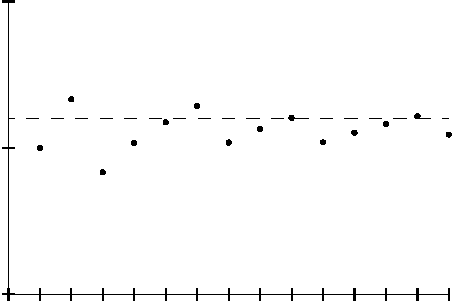
\includegraphics{figures/ser-rearrange}
\caption{The first 14 partial sums of the rearrangement convering
to $1.2$.\label{fig:serrearrange}}
\end{myfigureht}
\end{example}

\subsection{Multiplication of series}

As we have
already mentioned,
multiplication of series is somewhat harder than addition.
If at least one of the series converges
absolutely, then we can use the following theorem.  For this result, it is
convenient to start the series at 0, rather than at 1.

\begin{thm}[\myindex{Mertens' theorem}\footnote{Proved by
the German mathematician
\href{https://en.wikipedia.org/wiki/Franz_Mertens}{Franz Mertens}
(1840--1927).}]
Suppose $\sum_{n=0}^\infty a_n$ and $\sum_{n=0}^\infty b_n$ are two convergent series, converging
to $A$ and $B$ respectively.  Suppose at least one of the series
converges absolutely.  Define
\begin{equation*}
c_n \coloneqq a_0 b_n + a_1 b_{n-1} + \cdots + a_n b_0 = \sum_{i=0}^n a_i b_{n-i} .
\end{equation*}
Then the series $\sum_{n=0}^\infty c_n$
converges to $AB$.
\end{thm}

The series $\sum_{n=0}^\infty c_n$ is called the \emph{\myindex{Cauchy product}} of
$\sum_{n=0}^\infty a_n$ and $\sum_{n=0}^\infty b_n$.

\begin{proof}
Suppose $\sum_{n=0}^\infty a_n$ converges absolutely, and let $\epsilon > 0$ be
given.
In this proof instead of picking complicated estimates just to make
the final estimate come out as less than $\epsilon$,
let us simply obtain an estimate that depends on $\epsilon$
and can be made arbitrarily small.

Write
\begin{equation*}
A_m \coloneqq \sum_{n=0}^m a_n , \qquad B_m \coloneqq \sum_{n=0}^m b_n .
\end{equation*}
We rearrange the $m$th partial sum of $\sum_{n=0}^\infty c_n$:
\begin{equation*}
\begin{split}
\abs{\left(\sum_{n=0}^m c_n \right) - AB}
& =
\abs{\left( \sum_{n=0}^m \sum_{i=0}^n a_i b_{n-i} \right) - AB}
\\
& =
\abs{\left( \sum_{n=0}^m
  B_n a_{m-n} \right) - AB}
\\
& =
\abs{\left( \sum_{n=0}^m
  ( B_n -  B ) a_{m-n} \right)
    + B A_m - AB}
\\
& \leq
\left(
\sum_{n=0}^m
  \abs{ B_n -  B } \abs{a_{m-n}}
\right)
+
\abs{B}\abs{A_m - A}
\end{split}
\end{equation*}
We can surely make the second term on the right-hand side go to zero.
The trick is to handle the first term.
Pick $K$ such that for all $m \geq K$, we have 
$\abs{A_m - A} < \epsilon$ and
also
$\abs{B_m - B} < \epsilon$.  Finally,
as $\sum_{n=0}^\infty a_n$ converges absolutely,
make sure that $K$ is large enough such that
for all $m \geq K$,
\begin{equation*}
\sum_{n=K}^m \abs{a_n} < \epsilon .
\end{equation*}
As $\sum_{n=0}^\infty b_n$ converges, then
we have that
$B_{\text{max}} \coloneqq \sup \{ \abs{ B_n - B } : n = 0,1,2,\ldots \}$
is finite.  Take $m \geq 2K$, then in particular $m-K+1 > K$.  So
\begin{equation*}
\begin{split}
\sum_{n=0}^m
  \abs{ B_n -  B } \abs{a_{m-n}}
& =
\left(
\sum_{n=0}^{m-K}
  \abs{ B_n -  B } \abs{a_{m-n}}
\right)
+
\left(
\sum_{n=m-K+1}^m
  \abs{ B_n -  B } \abs{a_{m-n}}
\right)
\\
& \leq
\left(
\sum_{n=K}^m
\abs{a_{n}}
\right)
B_{\text{max}}
+
\left(
\sum_{n=0}^{K-1}
  \epsilon \abs{a_{n}}
\right)
\\
& \leq
\epsilon
B_{\text{max}}
+
\epsilon
\left(
\sum_{n=0}^\infty \abs{a_{n}}
\right) .
\end{split}
\end{equation*}
Therefore, for $m \geq 2K$, we have
\begin{equation*}
\begin{split}
\abs{\left(\sum_{n=0}^m c_n \right) - AB}
& \leq
\left(
\sum_{n=0}^m
  \abs{ B_n -  B } \abs{a_{m-n}}
\right)
+
\abs{B}\abs{A_m - A}
\\
& \leq
\epsilon
B_{\text{max}}
+
\epsilon
\left(
\sum_{n=0}^\infty \abs{a_{n}}
\right)
+
\abs{B}\epsilon
=
\epsilon 
\left(
B_{\text{max}}
+
\left(
\sum_{n=0}^\infty \abs{a_{n}}
\right)
+
\abs{B}
\right) .
\end{split}
\end{equation*}
The expression in the parenthesis on the right-hand side
is a fixed number.
Hence,
we can make the right-hand side arbitrarily small by picking a small enough
$\epsilon> 0$.  So $\sum_{n=0}^\infty c_n$ converges to $AB$.
\end{proof}

\begin{example}
If both series are only conditionally convergent, the Cauchy product series
need not even converge.
Suppose we take $a_n = b_n = {(-1)}^n \frac{1}{\sqrt{n+1}}$.
The series $\sum_{n=0}^\infty a_n = \sum_{n=0}^\infty b_n$
converges
by the alternating series test; however, it does not converge
absolutely as can be seen from the $p$-test.  Let us look
at the Cauchy product.
\begin{equation*}
c_n = 
{(-1)}^n
\left(
\frac{1}{\sqrt{n+1}} + 
\frac{1}{\sqrt{2n}} + 
\frac{1}{\sqrt{3(n-1)}} + \cdots +
%\frac{1}{\sqrt{2n}} + 
\frac{1}{\sqrt{n+1}}
\right)
=
{(-1)}^n
\sum_{i=0}^n \frac{1}{\sqrt{(i+1)(n-i+1)}} .
\end{equation*}
Therefore,
\begin{equation*}
\abs{c_n} 
=
\sum_{i=0}^n \frac{1}{\sqrt{(i+1)(n-i+1)}} 
\geq
\sum_{i=0}^n \frac{1}{\sqrt{(n+1)(n+1)}} 
= 1 .
\end{equation*}
The terms do not go to zero and hence $\sum_{n=0}^\infty c_n$ cannot converge.
\end{example}

\subsection{Power series}

Fix $x_0 \in \R$.
A \emph{\myindex{power series}} about $x_0$
is a series of the form
\begin{equation*}
\sum_{n=0}^\infty a_n {(x-x_0)}^n .
\end{equation*}
A power series is really a function of $x$, and
many important functions in analysis can be written
as a power series.  We use the convention that
$0^0 = 1$ (if $x=x_0$ and $n=0$).

A power series is said to be
\emph{convergent}\index{convergent!power series} if
there is at least one $x \not= x_0$ that makes the series converge.
If $x=x_0$, then the series always
converges since all terms except the first are zero.
If the series does not converge for any point $x \not= x_0$, we say that
the series is \emph{divergent}\index{divergent!power series}.

\begin{example} \label{ps:expex}
The series
\begin{equation*}
\sum_{n=0}^\infty \frac{1}{n!} x^n
\end{equation*}
is absolutely convergent for all $x \in \R$ using the ratio test:
For any $x \in \R$
\begin{equation*}
\lim_{n \to \infty}
\frac{\bigl(1/(n+1)!\bigr) \, x^{n+1}}{(1/n!) \, x^{n}}
=
\lim_{n \to \infty}
\frac{x}{n+1}
=
0.
\end{equation*}
Recall from calculus that this series converges to $e^x$.
\end{example}

\begin{example} \label{ps:1kex}
The series
\begin{equation*}
\sum_{n=1}^\infty \frac{1}{n} x^n
\end{equation*}
converges absolutely for all $x \in (-1,1)$ via the ratio test:
\begin{equation*}
\lim_{n \to \infty}
\abs{
\frac{\bigl(1/(n+1) \bigr) \, x^{n+1}}{(1/n) \, x^{n}}
}
=
\lim_{n \to \infty}
\abs{x} \frac{n}{n+1}
=
\abs{x} < 1 .
\end{equation*}
The series converges at $x=-1$,
as
$\sum_{n=1}^\infty \frac{{(-1)}^n}{n}$ converges
by the alternating series
test.
But the power series does not converge absolutely at $x=-1$, because
$\sum_{n=1}^\infty \frac{1}{n}$ does not converge.
The series
diverges at $x=1$.
When $\abs{x} > 1$, then the series diverges via the ratio test.
\end{example}

\begin{example} \label{ps:divergeex}
The series
\begin{equation*}
\sum_{n=1}^\infty n^n x^n
\end{equation*}
diverges for all $x \not= 0$.  Let us apply the root test
\begin{equation*}
\limsup_{n\to\infty}
\,
\abs{n^n x^n}^{1/n}
=
\limsup_{n\to\infty}
\,
n \abs{x}
= \infty .
\end{equation*}
Therefore, the series diverges for all $x \not= 0$.
\end{example}

Convergence of power series in general works analogously to
one of the three examples above.

\begin{prop} \label{prop:powerserrealradius}
Let $\sum_{n=0}^\infty a_n {(x-x_0)}^n$ be a power series.
If the series is convergent, then either it converges at
all $x \in \R$, or
there exists a number $\rho$, such that
the series converges absolutely on the interval
$(x_0-\rho,x_0+\rho)$ and diverges when $x < x_0-\rho$ or $x > x_0+\rho$.
\end{prop}

The number $\rho$ is called the \emph{\myindex{radius of convergence}} of the
power series.  We write $\rho = \infty$ if the series converges for
all $x$, and we write $\rho = 0$ if the series is divergent.
At the endpoints, that is if $x = x_0+\rho$ or $x = x_0-\rho$,
the proposition says nothing,
and the series might or might not converge.
See \figureref{ps:convfig}.
In \exampleref{ps:1kex}
the radius of convergence is $\rho=1$.
In \exampleref{ps:expex} the radius of convergence is $\rho=\infty$,
and in \exampleref{ps:divergeex} the radius of convergence is $\rho=0$.

\begin{myfigureht}
\subimport*{figures/}{ps-conv.pdf_t}
\caption{Convergence of a power series.\label{ps:convfig}}
\end{myfigureht}

\begin{proof}
Write
\begin{equation*}
R \coloneqq \limsup_{n\to\infty} {\abs{a_n}}^{1/n} .
\end{equation*}
We use the root test to prove the proposition:
\begin{equation*}
L = \limsup_{n\to\infty} {\abs{a_n {(x-x_0)}^n}}^{1/n} 
=
\abs{x-x_0} \limsup_{n\to\infty} {\abs{a_n}}^{1/n}
=
\abs{x-x_0} R .
\end{equation*}
In particular, if $R = \infty$, then $L=\infty$ for every $x \not= x_0$, and
the series diverges by the root test.
On the other hand,
if $R = 0$, then $L=0$ for every $x$,
and the series converges absolutely for all $x$.

Suppose $0 < R < \infty$.
The series
converges absolutely if
$1 > L = R \abs{x-x_0}$,
or in other words when
\begin{equation*}
\abs{x-x_0} < \nicefrac{1}{R} .
\end{equation*}
The series diverges when
$1 < L = R \abs{x-x_0}$,
or
\begin{equation*}
\abs{x-x_0} > \nicefrac{1}{R} .
\end{equation*}
Letting $\rho \coloneqq \nicefrac{1}{R}$ completes the proof.
\end{proof}

It may be useful to restate what we have learned in the proof
as a separate proposition.

\begin{prop}
Let $\sum_{n=0}^\infty a_n {(x-x_0)}^n$ be a power series, and let
\begin{equation*}
R \coloneqq \limsup_{n\to\infty} {\abs{a_n}}^{1/n} .
\end{equation*}
If $R = \infty$, the power series is divergent.  If
$R=0$, then the power series converges everywhere.   Otherwise,
the radius of convergence $\rho = \nicefrac{1}{R}$.
\end{prop}

Often, radius of convergence is written as $\rho = \nicefrac{1}{R}$ in all
three cases, with
the understanding of what $\rho$ should be if $R = 0$ or $R =
\infty$.

Convergent power series can be added and multiplied together, and multiplied
by constants.
The proposition has a straight forward proof using what we know about series
in general, and power series in particular.  We leave the proof to the reader.

\begin{prop}
Let $\sum_{n=0}^\infty a_n {(x-x_0)}^n$ and
$\sum_{n=0}^\infty b_n {(x-x_0)}^n$ be two convergent power series
with radius of convergence at least $\rho > 0$ and $\alpha \in \R$.  Then
for all $x$ such that $\abs{x-x_0} < \rho$, we have 
\begin{equation*}
\left(\sum_{n=0}^\infty a_n {(x-x_0)}^n\right)
+
\left(\sum_{n=0}^\infty b_n {(x-x_0)}^n\right)
=
\sum_{n=0}^\infty (a_n+b_n) {(x-x_0)}^n ,
\end{equation*}
\begin{equation*}
\alpha
\left(\sum_{n=0}^\infty a_n {(x-x_0)}^n\right)
=
\sum_{n=0}^\infty \alpha a_n {(x-x_0)}^n ,
\end{equation*}
and
\begin{equation*}
\left(\sum_{n=0}^\infty a_n {(x-x_0)}^n\right)
\,
\left(\sum_{n=0}^\infty b_n {(x-x_0)}^n\right)
=
\sum_{n=0}^\infty c_n {(x-x_0)}^n ,
\end{equation*}
where
$c_n = a_0b_n + a_1 b_{n-1} + \cdots + a_n b_0$.
\end{prop}

That is, after performing the algebraic operations, the
radius of convergence of the resulting series is at least $\rho$.
For all $x$ with $\abs{x-x_0} < \rho$, we have two convergent series so
their term by term addition and multiplication by constants
follows by what we learned in the last section.
For multiplication of two power series,
the series are absolutely convergent inside
the radius of convergence and that is why for those $x$
we can apply Mertens' theorem.
Note that after applying an algebraic operation the radius of convergence
could increase.  See the exercises.

Let us look at some examples of power series.
Polynomials are simply finite power series.  That is, a polynomial
is a power series where
the $a_n$ are zero for all $n$ large enough.  We expand
a polynomial as a power series about any point $x_0$ by writing
the polynomial as a polynomial in $(x-x_0)$.  For example,
$2x^2-3x+4$ as a power series around $x_0 = 1$ is
\begin{equation*}
2x^2-3x+4 = 3 + (x-1) + 2{(x-1)}^2 .
\end{equation*}

We can also expand
\emph{\myindex{rational functions}} (that is, ratios of polynomials)
as power series, although we will not completely prove this fact here.
Notice that a series for a rational function only defines the function
on an interval even if the function is defined elsewhere.  For example, for
the \emph{\myindex{geometric series}}, we have that for
$x \in (-1,1)$
\begin{equation*}
\frac{1}{1-x} =
\sum_{n=0}^\infty x^n .
\end{equation*}
The series diverges when $\abs{x} > 1$, even though $\frac{1}{1-x}$ is
defined for all $x \not= 1$.

We can use the geometric series together with rules for addition and
multiplication of power series to expand rational functions as power
series around $x_0$,
as long as the denominator is not zero at $x_0$.  We state without
proof that this is always possible, and we give an example of such
a computation using the geometric series.

\begin{example}
Let us expand $\frac{x}{1+2x+x^2}$ as a power series around the origin ($x_0 = 0$) and
find the radius of convergence.

Write $1+2x+x^2 = {(1+x)}^2 = {\bigl(1-(-x)\bigr)}^2$, and suppose
$\abs{x} < 1$.  Compute
\begin{equation*}
\begin{split}
\frac{x}{1+2x+x^2}
&=
x \,
{\left(
\frac{1}{1-(-x)}
\right)}^2
\\
&=
x \,
{\left( 
\sum_{n=0}^\infty {(-1)}^n x^n 
\right)}^2
\\
&=
x \,
\left(
\sum_{n=0}^\infty c_n x^n 
\right)
\\
&=
\sum_{n=0}^\infty c_n x^{n+1} .
\end{split}
\end{equation*}
Using the formula for the product of series,
we obtain $c_0 = 1$, $c_1 = -1 -1 = -2$, $c_2 = 1+1+1 = 3$, etc.
Hence, for $\abs{x} < 1$, 
\begin{equation*}
\frac{x}{1+2x+x^2}
=
\sum_{n=1}^\infty {(-1)}^{n+1} n x^n .
\end{equation*}
The radius of convergence is at least 1.  We leave it to the reader to
verify that the radius of convergence is exactly equal to 1.
\end{example}

You can use the method of partial fractions you know from calculus.
For example, to find the power series for $\frac{x^3+x}{x^2-1}$ at 0, write
\begin{equation*}
\frac{x^3+x}{x^2-1}
=
x + \frac{1}{1+x} - \frac{1}{1-x}
=
x + \sum_{n=0}^\infty {(-1)}^n x^n - \sum_{n=0}^\infty x^n .
\end{equation*}

\subsection{Exercises}

\begin{exercise}
Decide the convergence or divergence of the following series.

\medskip

\noindent
a)
$\displaystyle \sum_{n=1}^\infty \frac{1}{2^{2n+1}}$
\qquad
b)
$\displaystyle \sum_{n=1}^\infty \frac{{(-1)}^{n}(n-1)}{n}$
\qquad
c)
$\displaystyle \sum_{n=1}^\infty \frac{{(-1)}^n}{n^{1/10}}$
\qquad
d)
$\displaystyle \sum_{n=1}^\infty \frac{n^n}{{(n+1)}^{2n}}$
\end{exercise}

\begin{exercise}
Suppose both $\sum_{n=0}^\infty a_n$ and $\sum_{n=0}^\infty b_n$ 
converge absolutely.
Show that the product series, $\sum_{n=0}^\infty c_n$ where
$c_n = a_0 b_n + a_1 b_{n-1} + \cdots + a_n b_0$, also converges absolutely.
\end{exercise}

\begin{exercise}[Challenging] \label{exercise:seriesconvergestoanything}
Let $\sum_{n=1}^\infty a_n$ be conditionally convergent.
Show that given an arbitrary $x \in \R$
there exists a rearrangement of $\sum_{n=1}^\infty a_n$
such that the rearranged series converges to $x$.
Hint: See \exampleref{example:harmonsumanything}.
\end{exercise}

\begin{exercise}
\pagebreak[2]
\leavevmode
\begin{enumerate}[a)]
\item
Show that the alternating harmonic series $\sum_{n=1}^\infty \frac{{(-1)}^{n+1}}{n}$
has a rearrangement
such that for every interval $(x,y)$, there exists a partial sum $s_n$
of the rearranged series such that $s_n \in (x,y)$.
\item
Show that the rearrangement you found does not converge.
See \exampleref{example:harmonsumanything}.
\item
Show that for every $x \in \R$, there exists a subsequence of
partial sums $\{ s_{n_k} \}_{k=1}^\infty$ of your rearrangement such that 
$\lim\limits_{k\to\infty} s_{n_k} = x$.
\end{enumerate}
\end{exercise}

\begin{exercise}
For the following power series, find if they are convergent or not, and
if so find their radius of convergence.

\medskip

\noindent
a)
$\displaystyle \sum_{n=0}^\infty 2^n x^n$
\qquad
b) $\displaystyle \sum_{n=0}^\infty n x^n$
\qquad 
c) 
$\displaystyle \sum_{n=0}^\infty n! \, x^n$
\qquad
d) $\displaystyle \sum_{n=0}^\infty \frac{1}{(2n)!} {(x-10)}^n$
\qquad
e) $\displaystyle \sum_{n=0}^\infty x^{2n}$
\qquad
f) $\displaystyle \sum_{n=0}^\infty n! \, x^{n!}$
\end{exercise}

\begin{exercise}
Suppose $\sum_{n=0}^\infty a_n x^n$ converges for $x=1$.
\begin{enumerate}[a)]
\item
What can you say about the radius of convergence?
\item
If you further know that at $x=1$ the convergence is not absolute,
what can you say?
\end{enumerate}
\end{exercise}

\begin{exercise}
Expand
$\dfrac{x}{4-x^2}$ as a power series around $x_0 = 0$ and compute its radius
of convergence.
\end{exercise}

\begin{exercise}
\leavevmode
\begin{enumerate}[a)]
\item
Find an example where the radii of convergence of $\sum_{n=0}^\infty a_n x^n$ and
$\sum_{n=0}^\infty b_n x^n$ are both 1, but the radius of convergence of
the sum of the two series is infinite.
\item
(Trickier)
Find an example where the radii of convergence of $\sum_{n=0}^\infty a_n x^n$ and
$\sum_{n=0}^\infty b_n x^n$ are both 1, but the radius of convergence of
the product of the two series is infinite.
\end{enumerate}
\end{exercise}

\begin{exercise}
Figure out how to compute the radius of convergence using the ratio test.
That is, suppose $\sum_{n=0}^\infty a_n x^n$ is a power series and
$R \coloneqq \lim_{n\to\infty} \frac{\abs{a_{n+1}}}{\abs{a_n}}$ exists or is $\infty$.
Find the radius of convergence and prove your claim.
\end{exercise}

\begin{samepage}
\begin{exercise}
\leavevmode
\begin{enumerate}[a)]
\item
Prove that $\lim_{n\to\infty} n^{1/n} = 1$ using the following procedure:  Write $n^{1/n} = 1+b_n$ and
note $b_n > 0$.  Then show that ${(1+b_n)}^n \geq 
\frac{n(n-1)}{2}b_n^2$ and use this to show that $\lim\limits_{n\to\infty} b_n = 0$.
\item
Use the result of part a) to show that
if $\sum_{n=0}^\infty a_n x^n$ is a convergent power series with radius of convergence $R$,
then $\sum_{n=0}^\infty n a_n x^n$ is also convergent with the same radius of convergence.
\end{enumerate}
\end{exercise}
\end{samepage}

\begin{exnote}
There are different notions of summability (convergence)
of a series
than just the one we have seen.
A common one is \emph{\myindex{Ces\`aro summability}}%
\footnote{Named for the Italian mathematician
\href{https://en.wikipedia.org/wiki/Ernesto_Ces\%C3\%A0ro}{Ernesto Ces\`aro}
(1859--1906).}.  Let $\sum_{n=1}^\infty a_n$ be a series
and let $s_n$ be the $n$th partial sum.  The series is said to
be Ces\`aro summable to $a$ if
\begin{equation*}
a = \lim_{n\to \infty} \frac{s_1 + s_2 + \cdots + s_n}{n} .
\end{equation*}
\end{exnote}

\begin{exercise}[Challenging]
\pagebreak[2]
\leavevmode
\begin{enumerate}[a)]
\item
If $\sum_{n=1}^\infty a_n$ is convergent to $a$ (in the usual sense), show that
$\sum_{n=1}^\infty a_n$ is Ces\`aro summable (see above) to $a$.
\item
Show that in the sense of Ces\`aro $\sum_{n=1}^\infty {(-1)}^n$ is summable to
$\nicefrac{1}{2}$.
\item
Let $a_n \coloneqq k$ when $n = k^3$ for some $k \in \N$,
$a_n \coloneqq -k$ when $n = k^3+1$ for some $k \in \N$,
otherwise
let $a_n \coloneqq 0$.  Show that $\sum_{n=1}^\infty a_n$ diverges in the usual sense
(in fact, both the sequence of terms and the partial sums are unbounded), but it is
Ces\`aro summable to 0 (seems a little paradoxical at first sight).
\end{enumerate}
\end{exercise}

\begin{exercise}[Challenging]
Show that the monotonicity in the alternating series test
is necessary.  That is, find a sequence of positive real numbers
$\{ x_n \}_{n=1}^\infty$ with $\lim_{n\to\infty} x_n = 0$ but such that
$\sum_{n=1}^\infty {(-1)}^n x_n$ diverges.
\end{exercise}

\begin{exercise}
Find a series such that $\sum_{n=1}^\infty x_n$ converges,
but $\sum_{n=1}^\infty x_n^2$ diverges.
Hint: Compare \exerciseref{exercise:squareseriesconv}.
\end{exercise}

\begin{exercise}
Suppose $\{ c_n \}_{n=1}^\infty$ is a sequence.  Prove that for every $r \in (0,1)$,
there exists a strictly increasing sequence $\{ n_k \}_{k=1}^\infty$ of natural numbers
($n_{k+1} > n_k$) such that
\begin{equation*}
\sum_{k=1}^\infty c_k x^{n_k}
\end{equation*}
converges absolutely for all $x \in [-r,r]$.
\end{exercise}

